%
%   $Id$
%   This file is part of the FPC documentation.
%   Copyright (C) 1997, by Michael Van Canneyt
%
%   The FPC documentation is free text; you can redistribute it and/or
%   modify it under the terms of the GNU Library General Public License as
%   published by the Free Software Foundation; either version 2 of the
%   License, or (at your option) any later version.
%
%   The FPC Documentation is distributed in the hope that it will be useful,
%   but WITHOUT ANY WARRANTY; without even the implied warranty of
%   MERCHANTABILITY or FITNESS FOR A PARTICULAR PURPOSE.  See the GNU
%   Library General Public License for more details.
%
%   You should have received a copy of the GNU Library General Public
%   License along with the FPC documentation; see the file COPYING.LIB.  If not,
%   write to the Free Software Foundation, Inc., 59 Temple Place - Suite 330,
%   Boston, MA 02111-1307, USA.
%
\documentclass{report}
%
% Preamble
%
% Don't know why it's needed, but latex2html will else core dump
% when trying to create an image
\usepackage{epsfig}
\usepackage{multicol}
\ifx\pdfoutput\undefined
  \usepackage{html}
  \usepackage{htmllist}
  \latex{\usepackage{fpc}}
\else
  \usepackage{fpc}
\fi
%
\html{%
%   $Id$
%   This file is part of the FPC documentation.
%   Copyright (C) 1997, by Michael Van Canneyt
%
%   The FPC documentation is free text; you can redistribute it and/or
%   modify it under the terms of the GNU Library General Public License as
%   published by the Free Software Foundation; either version 2 of the
%   License, or (at your option) any later version.
%
%   The FPC Documentation is distributed in the hope that it will be useful,
%   but WITHOUT ANY WARRANTY; without even the implied warranty of
%   MERCHANTABILITY or FITNESS FOR A PARTICULAR PURPOSE.  See the GNU
%   Library General Public License for more details.
%
%   You should have received a copy of the GNU Library General Public
%   License along with the FPC documentation; see the file COPYING.LIB.  If not,
%   write to the Free Software Foundation, Inc., 59 Temple Place - Suite 330,
%   Boston, MA 02111-1307, USA. 
%
% Dummy
\newenvironment{FPCList}{\begin{description}}{\end{description}}
%
%
\newcommand{\Declaration}{\item[Declaration]\ttfamily}
\newcommand{\Description}{\item[Description]\rmfamily}
\newcommand{\Errors}{\item[Errors]\rmfamily}
\newcommand{\SeeAlso}{\item[See also]\rmfamily}
%
%  The environments
%
\newenvironment{functionl}[2]{\subsection{#1}%
\index{#1}\label{fu:#2}\begin{FPCList}}{\end{FPCList}}
\newenvironment{procedurel}[2]{\subsection{#1}%
\index{#1}\label{pro:#2}\begin{FPCList}}{\end{FPCList}}
\newenvironment{function}[1]{\begin{functionl}{#1}{#1}}{\end{functionl}}
\newenvironment{procedure}[1]{\begin{procedurel}{#1}{#1}}{\end{procedurel}}
\newcommand{\seefl}[2]{
\htmlref{#1}{fu:#2}
}
\newcommand{\seepl}[2]{
\htmlref{#1}{pro:#2}
}
%
% Now the ones without label.
%
\newcommand{\seef}[1]{\seefl{#1}{#1}}
\newcommand{\seep}[1]{\seepl{#1}{#1}}
%
\newcommand{\seet}[1]{
\htmlref{#1}{sec:types}
}
\newcommand{\seem}[2] {\texttt{#1} (#2) }
\newcommand{\var}[1]{\texttt {#1}}
\newcommand{\file}[1]{\textsf {#1}}
%
% Abbreviations
%
\newcommand{\linux}{\textsc{LinuX} }
\newcommand{\dos}  {\textsc{dos} }
\newcommand{\msdos}{\textsc{ms-dos} }
\newcommand{\ostwo}{\textsc{os/2} }
\newcommand{\windowsnt}{\textsc{WindowsNT} }
\newcommand{\windows}{\textsc{Windows} }
\newcommand{\docdescription}[1]{}
\newcommand{\docversion}[1]{}
\newcommand{\unitdescription}[1]{}
\newcommand{\unitversion}[1]{}
\newcommand{\fpc}{Free Pascal }
\newcommand{\gnu}{gnu }
%
% Useful references.
%
\newcommand{\progref}{\htmladdnormallink{Programmer's guide}{../prog/prog.html}\ }
\newcommand{\refref}{\htmladdnormallink{Reference guide}{../ref/ref.html}\ }
\newcommand{\userref}{\htmladdnormallink{Users' guide}{../user/user.html}\ }
\newcommand{\unitsref}{\htmladdnormallink{Unit reference}{../units/units.html}\ }
\newcommand{\seecrt}{\htmladdnormallink{CRT}{../crt/crt.html}}
\newcommand{\seelinux}{\htmladdnormallink{Linux}{../linux/linux.html}}
\newcommand{\seestrings}{\htmladdnormallink{strings}{../strings/strings.html}}
\newcommand{\seedos}{\htmladdnormallink{DOS}{../dos/dos.html}}
\newcommand{\seegetopts}{\htmladdnormallink{getopts}{../getopts/getopts.html}}
\newcommand{\seeobjects}{\htmladdnormallink{objects}{../objects/objects.html}}
\newcommand{\seegraph}{\htmladdnormallink{graph}{../graph/graph.html}}
\newcommand{\seeprinter}{\htmladdnormallink{printer}{../printer/printer.html}}
\newcommand{\seego}{\htmladdnormallink{GO32}{../go32/go32.html}}
%
% Nice environments
%
% For Code examples (complete programs only)
\newenvironment{CodEx}{}{}
% For Tables.
\newenvironment{FPCtable}[2]{\begin{table}\caption{#2}\begin{center}\begin{tabular}{#1}}{\end{tabular}\end{center}\end{table}}
% The same, but with label in third argument (tab:#3)
\newenvironment{FPCltable}[3]{\begin{table}\caption{#2}\label{tab:#3}\begin{center}\begin{tabular}{#1}}{\end{tabular}\end{center}\end{table}}
%
% Commands to reference these things.
%
\newcommand{\seet}[1]{table (\ref{tab:#1}) }
\newcommand{\seec}[1]{chapter (\ref{ch:#1}) }
\newcommand{\sees}[1]{section (\ref{se:#1}) }
}
%
\ifpdf
  \pdfinfo{/Author(Michael Van Canneyt)
           /Title(Users' Guide)
           /Subject(Free Pascal Users' guide)
           /Keywords(Free Pascal)
           }
\fi
%
% Settings
%
\makeindex
%
% Start of document.
%
\begin{document}
\title{Free Pascal :\\ Users' manual}
\docdescription{Users' manual for \fpc, version \fpcversion}
\docversion{1.8}
\input{date.inc}
\author{Micha\"el Van Canneyt\\Florian Kl\"ampfl}
\maketitle
\tableofcontents

%%%%%%%%%%%%%%%%%%%%%%%%%%%%%%%%%%%%%%%%%%%%%%%%%%%%%%%%%%%%%%%%%%%%%
% Introduction
%%%%%%%%%%%%%%%%%%%%%%%%%%%%%%%%%%%%%%%%%%%%%%%%%%%%%%%%%%%%%%%%%%%%%
\chapter{Introduction}

%%%%%%%%%%%%%%%%%%%%%%%%%%%%%%%%%%%%%%%%%%%%%%%%%%%%%%%%%%%%%%%%%%%%%%%
% About this document
\section{About this document}
This is the user's manual for \fpc . It describes the installation and
use of the \fpc compiler on the different supported platforms.
It does not attempt to give an exhaustive list of all supported commands,
nor a definition of the Pascal language. Look at the
\refref for these things.
For a description of the
possibilities and the inner workings of the compiler, see the
\progref . In the appendices of this document you will find lists of
reserved words and compiler error messages (with descriptions).

This document describes the compiler as it is/functions at the time of
writing. Since the compiler is under continuous development, some of the
things described here may be outdated. In case of doubt, consult the
\file{README} files, distributed with the compiler.
The \file{README} files are, in case of conflict with this manual,
authoritative.

%%%%%%%%%%%%%%%%%%%%%%%%%%%%%%%%%%%%%%%%%%%%%%%%%%%%%%%%%%%%%%%%%%%%%%%
% About the compiler
\section{About the compiler}
\fpc is a 32-bit compiler for the i386 and m68k processors\footnote{Work is being done
on a port to ALPHA Architecture}. Currently, it supports 7 operating systems:
\begin{itemize}
\item \dos
\item \linux
\item \atari (version 0.99.5 only)
\item \amiga (version 0.99.5 only)
\item \windows
\item \ostwo (using the EMX package, so it also works on DOS/Windows)
\item \freebsd (usable, but still under development).
\end{itemize}

\fpc is designed to be, as much as possible, source compatible with
Turbo Pascal 7.0 and Delphi 5 (although this goal is not yet attained),
but it also enhances these languages with elements like function overloading.
And, unlike these ancestors, it supports multiple platforms.

It also differs from them in the sense that you cannot use compiled units
from one system for the other.

Also, at the time of writing, there is only a early beta version of an
Integrated Development Environment (IDE) available for \fpc.

\fpc consists of three parts :
\begin{enumerate}
\item The compiler program itself.
\item The Run-Time Library (RTL).
\item Utility programs and units.
\end{enumerate}

Of these you only need the first two, in order to be able to use the compiler.
In this document, we describe the use of the compiler. The RTL is described in the
\refref.

%%%%%%%%%%%%%%%%%%%%%%%%%%%%%%%%%%%%%%%%%%%%%%%%%%%%%%%%%%%%%%%%%%%%%%%
% Getting more information.
\section{Getting more information.}
If the documentation doesn't give an answer to your questions,
you can obtain more information on the Internet, on the following addresses:
\begin{itemize}
\item
\htmladdnormallink{http://www.freepascal.org/}
{http://www.freepascal.org} is the main
site. It contains also useful mail addresses and
links to other places.
It also contains the instructions for inscribing to the
\textit{mailing-list}.

\item
\htmladdnormallink{http://www.brain.uni-freiburg.de/\~{}klaus/fpc/fpc.html}
{http://www.brain.uni-freiburg.de/\~{}klaus/fpc/fpc.html} is a mirror
of the main \fpc information site.
\end{itemize}
Both places can be used to download the \fpc distribution, although you can
probably find them on other places also.

Finally, if you think something should be added to this manual
(entirely possible), please do not hesitate and contact me at
\htmladdnormallink{michael@freepascal.org}{mailto:michael@freepascal.org}.
.

Let's get on with something useful.

%%%%%%%%%%%%%%%%%%%%%%%%%%%%%%%%%%%%%%%%%%%%%%%%%%%%%%%%%%%%%%%%%%%%%
% Installation
%%%%%%%%%%%%%%%%%%%%%%%%%%%%%%%%%%%%%%%%%%%%%%%%%%%%%%%%%%%%%%%%%%%%%

\chapter{Installing the compiler}
\label{ch:Installation}

%%%%%%%%%%%%%%%%%%%%%%%%%%%%%%%%%%%%%%%%%%%%%%%%%%%%%%%%%%%%%%%%%%%%%%%
% Before Installation : Requirements
\section{Before Installation : Requirements}

%
% System requirements
%
\subsection{System requirements}
The compiler needs at least the following hardware:
\begin{enumerate}
\item An I386 or higher processor. A coprocessor is not required, although it
will slow down your program's performance if you do floating point calculations
without a coprocessor, since an emulation will be used.
\item 4 Mb of free memory. Under \dos, if you use DPMI memory management,
such as under Windows, you will need at least 16 Mb.
\item At least 500 Kb. free disk space.
\end{enumerate}

% Software requirements
\subsection{Software requirements}

\subsubsection{Under DOS}
The \dos distribution contains all the files you need to run the compiler
and compile pascal programs.

\subsubsection{Under Linux}
Under \linux you need to have the following programs installed :
\begin{enumerate}
\item \gnu \file{as}, the \gnu assembler.
\item \gnu \file{ld}, the \gnu linker.
\item Optionally (but highly recommended) : \gnu \file{make}. For easy
recompiling of the compiler and Run-Time Library, this is needed.
\end{enumerate}
Other than that, \fpc should run on almost any I386 \linux system.

\subsubsection{Under Windows}
The \windows distribution contains all the files you need to run the compiler
and compile pascal programs. However, it may be a good idea to install
the \file{mingw32} tools or the \var{cygwin} development tools. Links
to both of these tools can be found on \var{http://www.freepascal.org}

\subsubsection{Under OS/2}
While the \fpc distribution comes with all necessary tools, it is a good
idea to install the EMX extender in order to compile and run
programs with the Free Pascal compiler. The EMX extender can be found on:\\
\var{http://www.leo.org/pub/comp/os/os2/leo/gnu/emx+gcc/index.html}

%%%%%%%%%%%%%%%%%%%%%%%%%%%%%%%%%%%%%%%%%%%%%%%%%%%%%%%%%%%%%%%%%%%%%%%
% Installing the compiler.
\section{Installing the compiler.}
The installation of \fpc is easy, but is platform-dependent.
We discuss the process for each platform separately.

% Installing under DOS
\subsection{Installing under DOS or Windows}
\subsubsection{Mandatory installation steps.}
First, you must get the latest distribution files of \fpc. They come as zip
files, which you must unzip first, or you can download the compiler as a
series of separate files. This is especially useful if you have a slow
connection, but it is also nice if you want to install only some pats of the
compiler distribution.  The distribution zip file contains an
installation program \file{INSTALL.EXE}. You must run this program to install
the compiler.

\begin{htmlonly}
The first screen of the installation program looks like this:
\htmladdimg{../pics/install1.gif}
And the second screen looks like
\htmladdimg{../pics/install2.gif}
\end{htmlonly}
\begin{latexonly}
The screen of the installation program looks like figure \ref{fig:install}.
\begin{figure}
\caption{The \dos install program screen.}
\label{fig:install}
\ifpdf
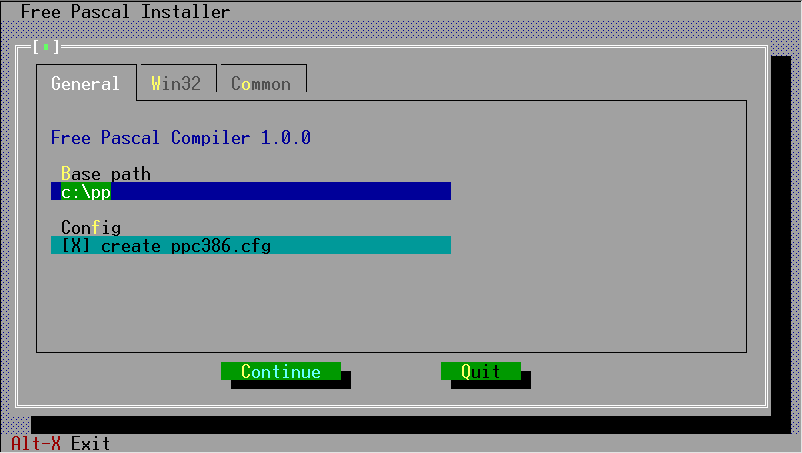
\epsfig{file=pics/install1.png,width=\textwidth}
%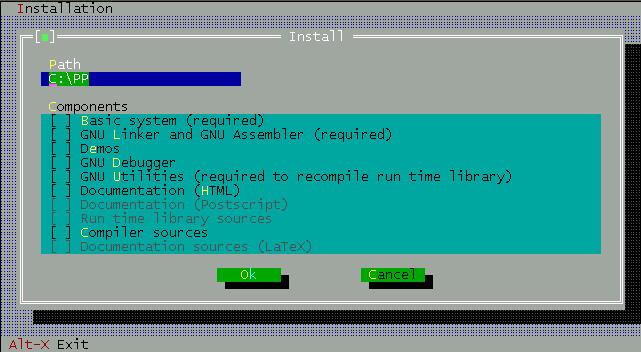
\epsfig{file=pics/install.png,width=\textwidth}
\end{figure}
\begin{figure}
\caption{The \dos install program screen.}
\label{fig:installb}
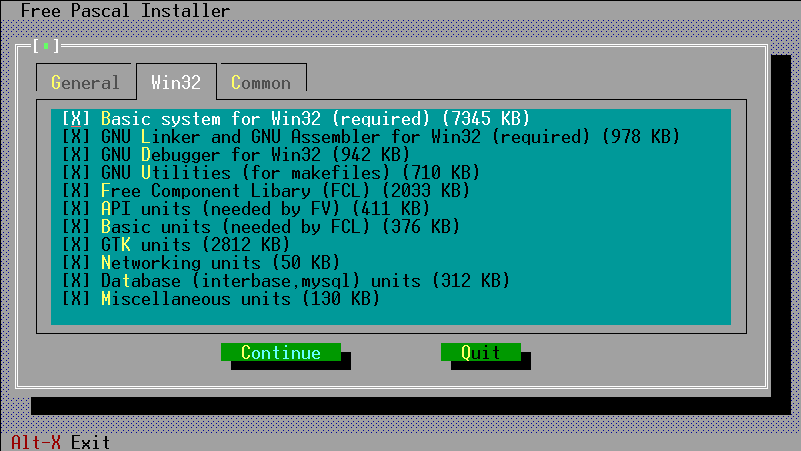
\epsfig{file=pics/install2.png,width=\textwidth}
%\epsfig{file=pics/install2s.png}
\else
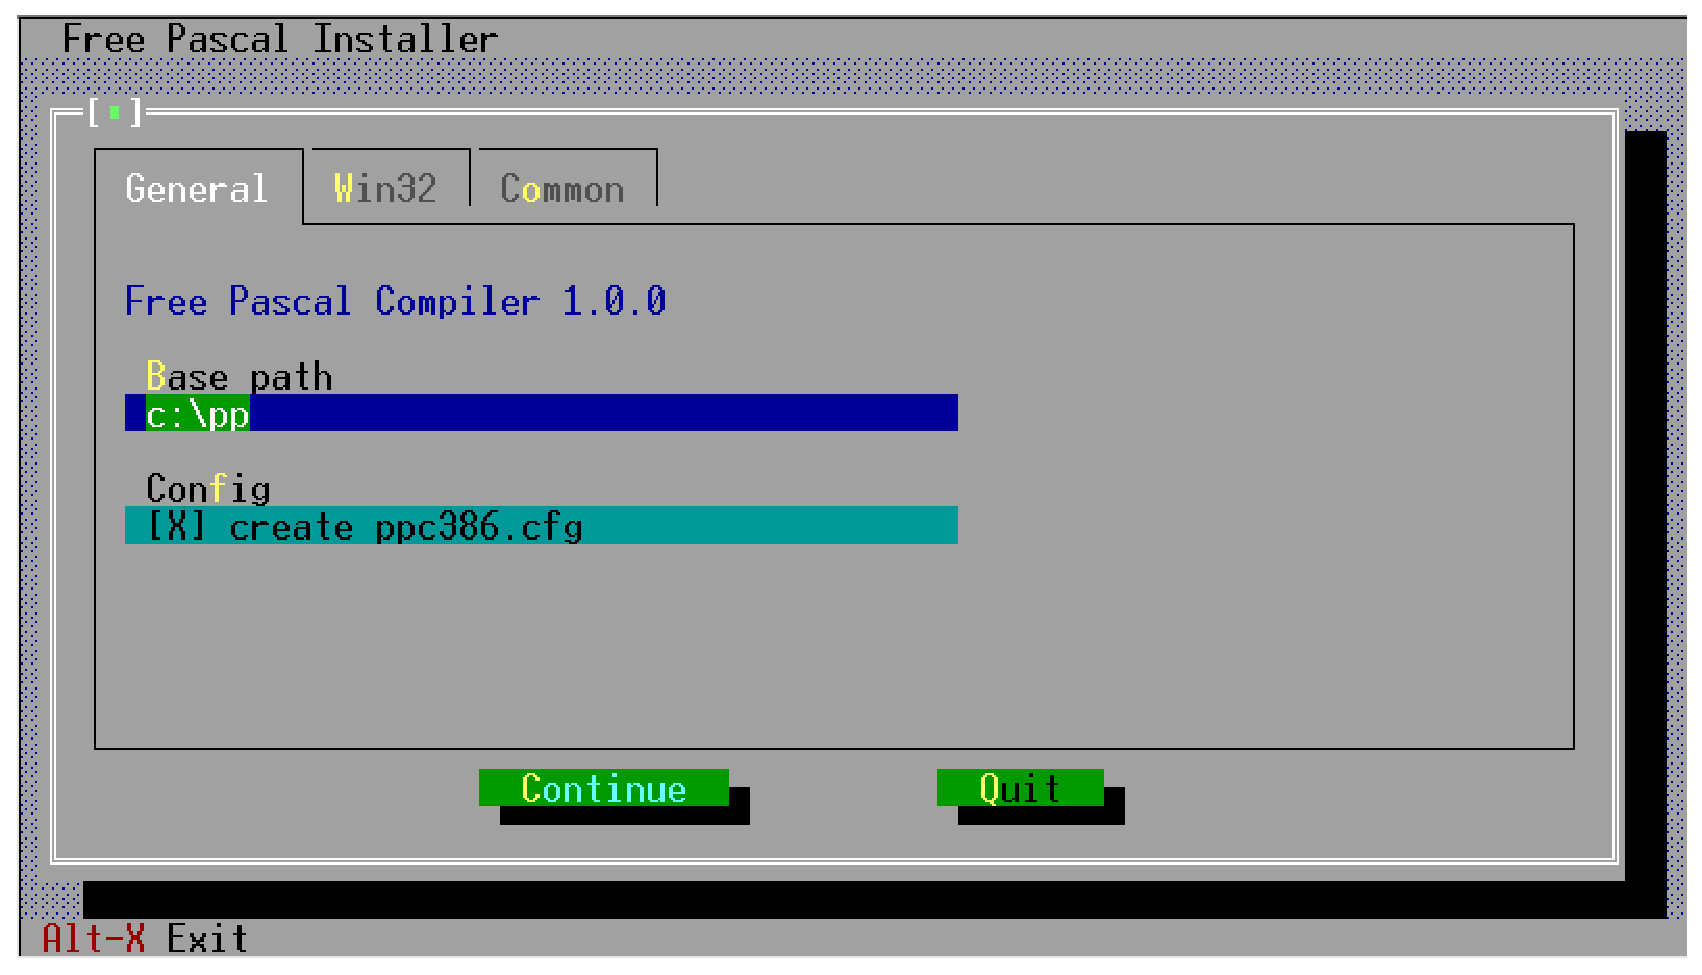
\epsfig{file=pics/install1.eps,width=\textwidth}
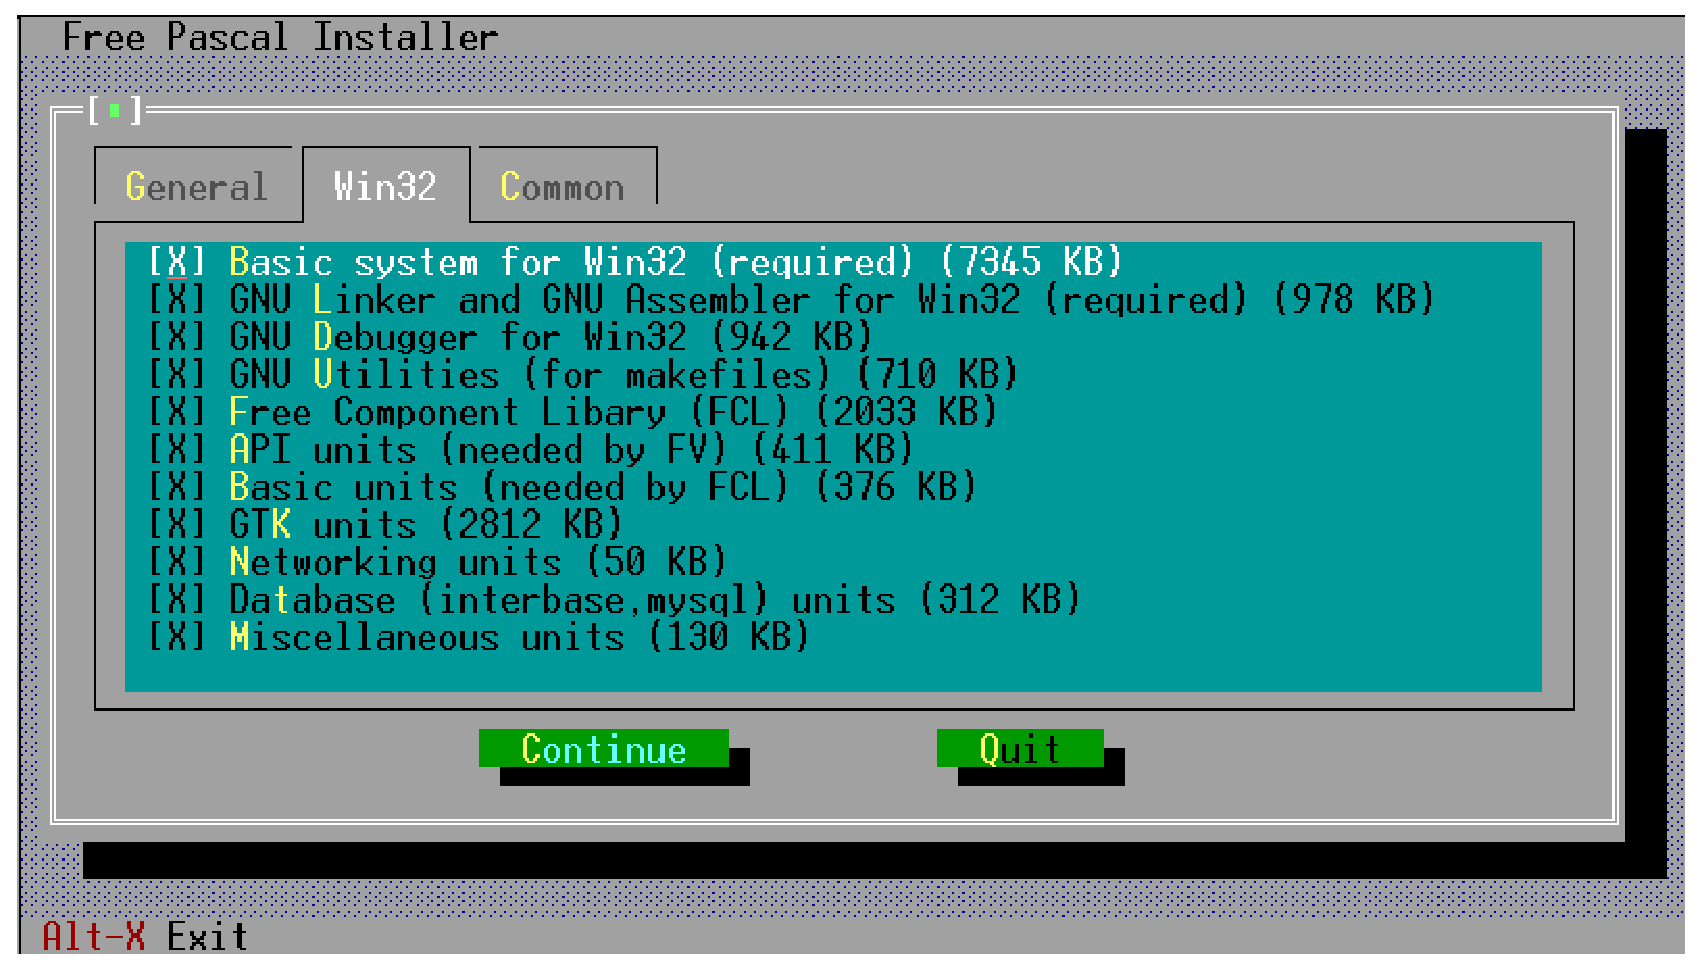
\epsfig{file=pics/install2.eps,width=\textwidth}
\fi
\end{figure}
\end{latexonly}

The program allows you to select:
\begin{itemize}
\item What components you wish to install. e.g do you want the sources or
not, do you want docs or not. Items that you didn't download when
downloading as separate files, will not be enabled, i.e. you can't
select them.

\item Where you want to install (the default location is \verb|C:\PP|).
\end{itemize}

In order to run \fpc from any directory on your system, you must extend
your path variable to contain the \verb|C:\PP\BIN| directory.
Usually this is done in the \file{AUTOEXEC.BAT} file.
It should look something like this :
\begin{verbatim}
  SET PATH=%PATH%;C:\PP\BIN
\end{verbatim}
(Again, assuming that you installed in the default location).

If you want to use the graphic drivers you must modify the
environment variable \var{GO32}. Instructions for doing this can be found
in the documentation of the Graph unit, at the \var{InitGraph} procedure.

\subsubsection{Optional Installation: The coprocessor emulation}
For people who have an older CPU type, without math coprocessor (i387)
it is necessary to install a coprocessor emulation, since \fpc uses the
coprocessor to do all floating point operations.

The installation of the coprocessor emulation is handled by the
installation program (\file{INSTALL.EXE}) under \dos and \windows.

%
% Installing under Linux
%
\subsection{Installing under Linux}
\subsubsection{Mandatory installation steps.}
The \linux distribution of \fpc comes in three forms:
\begin{itemize}
\item a \file{tar.gz} version, also available as seperate files.
\item a \file{.rpm} (Red Hat Package Manager) version, and
\item a \file{.deb} (debian) version.
\end{itemize}
All of these packages contain a \var{ELF} version of the compiler binaries and
units. the older \var{aout} binaries are no longer distributed, although you
still can use the comiler on an \var{aout} system if you recompile it.

If you use the \file{.rpm} format, installation is limited to
\begin{verbatim}
rpm -i fpc-pascal-XXX.rpm
\end{verbatim}
(\var{XXX} is the version number of the \file{.rpm} file)

If you use debian, installation is limited to
\begin{verbatim}
dpkg -i fpc-XXX.deb
\end{verbatim}
Here again, \var{XXX} is the version number of the \file{.deb} file.

You need root access to install these packages. The \file{.tar} file
allows you to do an installation if you don't have root permissions.

When downloading the \var{.tar} file, or the separate files,
 installation is more interactive.

In case you downloaded the \file{.tar} file, you should first untar
the file, in some directory where
you have write permission, using the following command:
\begin{verbatim}
tar -xvf fpc.tar
\end{verbatim}
We supposed here that you downloaded the file \file{fpc.tar} somewhere
from the Internet. (The real filename will have some version number in it,
which we omit here for clarity.)

When the file is untarred, you will be left with more archive files, and
an install program: an installation shell script.

If you downloaded the files as separate files, you should at least download
the \file{install.sh} script, and the libraries (in \file{libs.tar.gz}).

To install \fpc, all that you need to do now is give the following command:
\begin{verbatim}
./install.sh
\end{verbatim}
And then you must answer some questions. They're very simple, they're
mainly concerned with 2 things :
\begin{enumerate}
\item Places where you can install different things.
\item Deciding if you want to install certain components (such as sources
and demo programs).
\end{enumerate}
The script will automatically detect which components are present and can be
installed. It will only offer to install what has been found.
because of this feature, you must keep the original names when downloading,
since the script expects this.

If you run the installation script as the \var{root} user, you can just accept all installation
defaults. If you don't run as \var{root}, you must take care to supply the
installation program with directory names where you have write permission,
as it will attempt to create the directories you specify.
In principle, you can install it wherever you want, though.

At the end of installation, the installation program will generate a
configuration file for the \fpc compiler which reflects the settings
that you chose. It will install this file in the \file{/etc} directory, (if
you are not installing as \var{root}, this will fail), and in the
directory where you installed the libraries.

If you want the \fpc compiler to use this configuration file, it must be
present in \file{/etc}, or you can set the environment variable
\var{PPC\_CONFIG\_PATH}. Under \file{csh}, you can do this by adding  a
\begin{verbatim}
setenv PPC_CONFIG_PATH /usr/lib/ppc/0.99.14
\end{verbatim}
line to your \file{.login} file in your home directory.
(see also the next section)

\section{Optional configuration steps}
On any platform, after installing the compiler you may wish to set
some environment variables. The \fpc compiler
recognizes the following variables :
\begin{itemize}
\item \verb|PPC_EXEC_PATH| contains the directory where '\file{as}' and
'\file{ld}' are. (default \file{/usr/bin})
\item \verb|PPC_GCCLIB_PATH| contains the directory where \file{libgcc.a}
is (no default). This if for \linux only.
\item \verb|PPC_CONFIG_PATH| specifies an alternate path to find
\file{ppc386.cfg} (default under \linux is \file{/etc})
\item \verb|PPC_ERROR_FILE|  specifies the path and name of the error-definition file.
                  (default \file{/usr/lib/fpc/errorE.msg})
\end{itemize}

These locations are, however, set in the sample configuration file which is
built at the end of the installation process, except for the
\verb|PPC_CONFIG_PATH| variable, which you must set if you didn't install
things in the default places.
\subsubsection{finally}
Also distributed in \fpc is a README file. It contains the latest
instructions for installing \fpc, and should always be read first.


%%%%%%%%%%%%%%%%%%%%%%%%%%%%%%%%%%%%%%%%%%%%%%%%%%%%%%%%%%%%%%%%%%%%%%%
% Testing the compiler
\section{Testing the compiler}
After the installation is completed and the environment variables are
set as described above, your first program can be compiled.

Included in the \fpc distribution are some demonstration programs,
showing what the compiler can do.
You can test if the compiler functions correctly by trying to compile
these programs.

The compiler is called
\begin{itemize}
\item \file{ppc386} under \linux
\item \file{PPC386.EXE} under other target systems.
\end{itemize}
To compile a program (e.g \verb|demo\hello.pp|) simply type :
\begin{verbatim}
  ppc386 hello
\end{verbatim}
at the command prompt. If you don't have a configuration file, then you may
need to tell the compiler where it can find the units, for instance as
follows:
\begin{verbatim}
ppc386 -Fuc:\pp\units\go32v2\rtl hello
\end{verbatim}
under \dos, and under \linux you could type
\begin{verbatim}
ppc386 -Fu/usr/lib/fpc/0.99.14/units/linux/rtl hello
\end{verbatim}
This is, of course, assuming that you installed under \verb|C:\PP| or
\file{/usr/lib/fpc/0.99.14}, respectively.

If you got no error messages, the compiler has generated an executable
called \file{hello} (no extension) under \linux, and a file \file{hello.exe}
under \dos.

To execute the program, simply type :
\begin{verbatim}
  hello
\end{verbatim}
If all went well, you should see the following friendly greeting:
\begin{verbatim}
Hello world
\end{verbatim}

%%%%%%%%%%%%%%%%%%%%%%%%%%%%%%%%%%%%%%%%%%%%%%%%%%%%%%%%%%%%%%%%%%%%%
% Usage
%%%%%%%%%%%%%%%%%%%%%%%%%%%%%%%%%%%%%%%%%%%%%%%%%%%%%%%%%%%%%%%%%%%%%
\chapter{Compiler usage}
\label{ch:Usage}

Here we describe the essentials to compile a program and a unit.
We also describe how to make a stand-alone executable of the
compiled program under \dos. For more advanced uses of the compiler,
see the section on configuring the compiler, and the
\progref{}.

The examples in this section suppose that you have a \file{ppc386.cfg} which
is set up correctly, and which contains at least the path setting for the
RTL units. In principle this file is generated by the installation program.
You may have to check that it is in the correct place (see section
\ref{se:configfile} for more information on this).

%%%%%%%%%%%%%%%%%%%%%%%%%%%%%%%%%%%%%%%%%%%%%%%%%%%%%%%%%%%%%%%%%%%%%%%
% Where the compiler looks for its files.
\section{File searching}
Before you start compiling a program or a series of units, it is
important to know where the compiler looks for its source files and other
files. In this section we discuss this, and we indicate how to influence
this.

\begin{remark}
The use of slashes (/) and backslashes (\verb+\+) as directory separators
is irrelevant, the compiler will convert to whatever character is used on
the current operating system. Examples will be given using slashes, since
this avoids problems on \linux.
\end{remark}

% Command-line files.
\subsection{Command line files}
The file that you specify on the command line, such as in
\begin{verbatim}
ppc386 foo.pp
\end{verbatim}
will be looked for ONLY in the current directory. If you specify a directory
in the filename, then the compiler will look in that directory:
\begin{verbatim}
ppc386 subdir/foo.pp
\end{verbatim}
will look for \file{foo.pp} in the subdirectory \file{subdir} of the current
directory.

Under \linux, the name of this file is case sensitive, under other operating
systems (\dos, \windowsnt, \ostwo) this is not the case.

% Unit files.
\subsection{Unit files}

When you compile a unit or program that needs other units, the compiler will
look for compiled versions of these units in the following way:
\begin{enumerate}
\item It will look in the current directory.
\item It will look in the directory where the compiler binary is.
(not under \linux)
\item It will look in all the directories specified in the unit search path.
\end{enumerate}
You can add a directory to the unit search path with the \var{-Fu} option
(\seeo{Fu}). Every occurrence of one of this options will {\em insert}
a directory to the unit search path. i.e. last path on the command line
will be searched first.

The compiler adds several paths to the unit search path:
\begin{enumerate}
\item The contents of the environment variable \var{XXUNITS}, where \var{XX}
musrt be replaced with one of the supported targets: \var{GO32V2},
\var{LINUX},\var{WIN32}, \var{OS2}.
\item The standard unit directory. This directory is determined
from the \var{FPCDIR} environment variable. If this variable is not set,
then it is defaulted to the following:
\begin{itemize}
\item On \linux:
\begin{verbatim}
  /usr/local/lib/fpc/VERSION
or
  /usr/lib/fpc/VERSION
\end{verbatim}
whichever is found first.
\item On other OSes: the compiler binary directory, with '../' appended
to it, if it exists.
\end{itemize}
After this directory is determined , the following paths are added to the
search path:
\begin{enumerate}
\item FPCDIR/units/TARGET
\item FPCDIR/units/TARGET/rtl
\end{enumerate}
Here target must be replaced by the name of the target you are compiling for.
\end{enumerate}
You can see what paths the compiler will search by giving the compiler
the \var{-vu} option.

On \linux, the compiler will first convert the filename of a unit to
all-lowercase. This is necessary, since Pascal is case-independent, and
the statements \var{Uses Unit1;} or \var{uses unit1;} should have the same
effect.
Also, unit names that are longer than 8 characters will first be looked for
with their full length. If the unit is not found with this name, the name
will be truncated to 8 characters, and the compiler will look again in the
same directories, but with the truncated name.

For instance, suppose that the file \file{foo.pp} needs the unit
\file{bar}. Then the command
\begin{verbatim}
ppc386 -Fu.. -Fuunits foo.pp
\end{verbatim}
will tell the compiler to look for the unit \file{bar} in the following
places:
\begin{enumerate}
\item In the current directory.
\item In the directory where the compile binary is (not under \linux).
\item In the parent directory of the current directory.
\item In the subdirectory \file{units} of the current directory
\item In the standard unit directory.
\end{enumerate}

If the compiler finds the unit it needs, it will look for the source file of
this unit in the same directory where it found the unit.
If it finds the source of the unit, then it will compare the file times.
If the source file was modified more recent than the unit file, the
compiler will attempt to recompile the unit with this source file.

If the compiler doesn't find a compiled version of the unit, or when the
\var{-B} option is specified, then the compiler will look in the same
manner for the unit source file, and attempt to recompile it.

It is recommended to set the unit search path in the configuration file
\file{ppc386.cfg}. If you do this, you don't need to specify the unit search
path on the command-line every time you want to compile something.

% Include files.
\subsection{Include files}
If you include files in your source with the \var{\{\$I filename\}}
directive, the compiler will look for it in the following places:

\begin{enumerate}
\item It will look in the path specified in the incude file name.
\item It will look in the directory where the current source file is.
\item it will look in all directories specified in the include file search
path.
\end{enumerate}
You can add files to the include file search
 path with the \var{-I} (\seeo{I})
option.

As an example, consider the following include statement in a file
\file{units/foo.pp}:
\begin{verbatim}

{$i ../bar.inc}

\end{verbatim}
Then the following command :
\begin{verbatim}
ppc386 -Iincfiles units/foo.pp
\end{verbatim}
will cause the compiler to look in the following directories for
\file{bar.inc}:
\begin{enumerate}
\item the parent directory of the current directory
\item the \file{units} subdirectory of the current directory
\item the \file{incfiles} directory of the current directory.
\end{enumerate}

% Object files.
\subsection{Object files}
When you link to object files (using the \var{\{\$L file.o\}} directive,
the compiler will look for this file in the same way as it looks for include
files:

\begin{enumerate}
\item It will look in the path specified in the object file name.
\item It will look in the directory where the current source file is.
\item it will look in all directories specified in the object file search path.
\end{enumerate}
You can add files to the object file search path with the \var{-Fo} (\seeo{Fo})
option.

% Configuration file
\subsection{Configuration file}
\label{searchconfig}
Unless you specify the \var{-n} (\seeo{n}) option, the compiler will look
for a configuration file \file{ppc386.cfg} in the following places:

\begin{itemize}
\item Under \linux
\begin{enumerate}
\item The current directory.
\item In your home directory, it looks for \file{.ppc386.cfg}.
\item The directory specified in the environment variable
\var{PPC\_CONFIG\_PATH}, and if it's not set under \file{/etc}.
\end{enumerate}
\item Under all other OSes:
\begin{enumerate}
\item The current directory.
\item If it is set, the directory specified in the environment variable.
\var{PPC\_CONFIG\_PATH}.
\item The directory where the compiler is.
\end{enumerate}
\end{itemize}

\subsection{About long filenames}
\fpc can handle long filenames under \windows; it will use support for
long filenames if it is available.

If no support for long filenames is present, it will truncate unit names
to 8 characters.

It is not recommended to put units in directories that contain spaces in
their names, since the linker doesn't understand such filenames.

%%%%%%%%%%%%%%%%%%%%%%%%%%%%%%%%%%%%%%%%%%%%%%%%%%%%%%%%%%%%%%%%%%%%%%%
% Compiling a program
\section{Compiling a program}
Compiling a program is very simple. Assuming that you have a program source
in the file \file{prog.pp}, you can compile this with the following command:
\begin{verbatim}
  ppc386 [options] prog.pp
\end{verbatim}
The square brackets \var{[\ ]} indicate that what is between them is optional.

If your program file has the \file{.pp} or \file{.pas} extension,
you can omit this on the command line, e.g. in the previous example you
could have typed:
\begin{verbatim}
  ppc386 [options] prog
\end{verbatim}

If all went well, the compiler will produce an executable, or, for version 1
of the \dos extender, a file which can be converted to an executable.

Unless you are using \dos and version 1 of the \dos extender,
the file you obtained is the executable.
You can execute it straight away, you don't need to do
anything else. Under version 1 of the \dos extender,
additional processing is required. See section \ref{go32v1} on how to
create an executable in this case.

You will notice that there is also another file in your directory, with
extensions \file{.o}. This contains the object file for your program.
If you compiled a program, you can delete the object file (\file{.o}),
but not if you compiled a unit.
Then the object file contains the code of the unit, and will be
linked in any program that uses the unit you compiled, so you shouldn't
remove it.


%%%%%%%%%%%%%%%%%%%%%%%%%%%%%%%%%%%%%%%%%%%%%%%%%%%%%%%%%%%%%%%%%%%%%%%
% Compiling a unit
\section{Compiling a unit}

Compiling a unit is not essentially different from compiling a program.
The difference is mainly that the linker isn't called in this case.

To compile a unit in the file \file{foo.pp}, just type :
\begin{verbatim}
  ppc386  foo
\end{verbatim}
Recall the remark about file extensions in the previous section.

When all went well, you will be left with 2 (two) unit files:
\begin{enumerate}
\item \file{foo.ppu} This is the file describing the unit you just
compiled.
\item \file{foo.o} This file contains the actual code of the unit.
This file will eventually end up in the executables.
\end{enumerate}
Both files are needed if you plan to use the unit for some programs.
So don't delete them. If you want to distribute the unit, you must
provide both the \file{.ppu} and \file{.o} file. One is useless without the
other.

\begin{remark}
Under \linux, a unit source file {\em must} have a lowercase filename.
Since Pascal is case independent, you can specify the names of units in the
\var{uses} clause in either case. To get a unique filename, the \fpc compiler
changes the name of the unit to all lowercase when looking for unit files.
\end{remark}
The compiler produces lowercase files, so your unit will be found, even if
your source file has uppercase letters in it. Only when the compiler tries to
recompile the unit, it will not find your source because of the uppercase
letters.

%%%%%%%%%%%%%%%%%%%%%%%%%%%%%%%%%%%%%%%%%%%%%%%%%%%%%%%%%%%%%%%%%%%%%%%
% Units libraries and smartlinking
\section{Units, libraries and smartlinking}
The \fpc compiler supports smartlinking and the creation of libraries.
However, the default behaviour is to compile each unit into 1 big object
file, which will be linked as a whole into your program.

Not only is it possible to compile a shared library under \windows and
\linux, but also it is possible to take existing units and put them
together in 1 static or shared library (using the \file{ppumove} tool)

%%%%%%%%%%%%%%%%%%%%%%%%%%%%%%%%%%%%%%%%%%%%%%%%%%%%%%%%%%%%%%%%%%%%%%%
% Creating an executable for GO32V1, PMODE/DJ targets
\section{Creating an executable for GO32V1 and PMODE/DJ targets}
\label{go32v1}

The GO32V1 platform is officially no longer supported, so this section
is of interest only to people who wish to make go32V1 binaries anyway.

%
% GO32V1
%
\subsection{GO32V1}
When compiling under \dos, GO32V2 is the default target. However, if you use
go32V1 (using the \var{-TGO32V1} switch), the
compilation process leaves you with a file which you cannot execute right away.
There are 2 things you can do when compiling has finished.

The first thing is to use the \dos extender from D.J. Delorie to execute
your program :
\begin{verbatim}
  go32 prog
\end{verbatim}
This is fine for testing, but if you want to use a program regularly, it
would be easier if you could just type the program name, i.e.
\begin{verbatim}
  prog
\end{verbatim}
This can be accomplished by making a \dos executable of your compiled program.

There two ways to create a \dos executable (under \dos only):
\begin{enumerate}
\item if the \file{GO32.EXE} is already
installed on the computers where the program should run, you must
only copy a program called \file{STUB.EXE} at the begin of
the AOUT file. This is accomplished with the \file{AOUT2EXE.EXE} program.
which comes with the compiler:
\begin{verbatim}
AOUT2EXE PROG
\end{verbatim}
and you get a \dos executable which loads the \file{GO32.EXE} automatically.
the \file{GO32.EXE} executable must be in current directory or be
in a directory in the \var{PATH} variable.
\item
The second way to create a \dos executable is to put
\file{GO32.EXE} at the beginning of the \file{AOUT} file. To do this, at the
command prompt, type :
\begin{verbatim}
COPY /B GO32.EXE+PROG PROG.EXE
\end{verbatim}
(assuming \fpc created a file called \file{PROG}, of course.)
This becomes then a stand-alone executable for \dos, which doesn't need the
\file{GO32.EXE} on the machine where it should run.
\end{enumerate}

%
%

% PMODE/DJ
\subsection{PMODE/DJ}
You can also use the PMODE/DJ extender to run your \fpc applications.
To make an executable which works with the PMODE extender, you can simply
create an GO32V2 executable (the default), and then convert it to a PMODE
executable with the following two extra commands:
\begin{enumerate}
\item First, strip the GO32V2 header of the executable:
\begin{verbatim}
EXE2COFF PROG.EXE
\end{verbatim}
(we suppose that \file{PROG.EXE} is the program generated by the compilation
process.
\item Secondly, add the PMODE stub:
\begin{verbatim}
COPY /B PMODSTUB.EXE+PROG PROG.EXE
\end{verbatim}
If the \file{PMODSTUB.EXE} file isn't in your local directory, you need to
supply the whole path to it.
\end{enumerate}

That's it. No additional steps are needed to create a PMODE extender
executable.

Be aware, though, that the PMODE extender doesn't support virtual memory, so
if you're short on memory, you may run unto trouble. Also, officially there
is not support for the PMODE/DJ extender. It just happens that the compiler
and some of the programs it generates, run under this extender too.


%%%%%%%%%%%%%%%%%%%%%%%%%%%%%%%%%%%%%%%%%%%%%%%%%%%%%%%%%%%%%%%%%%%%%%%
% Reducing the size of your program
\section{Reducing the size of your program}

When you created your program, it is possible to reduce its size. This
is possible, because the compiler leaves a lot of information in the
program which, strictly speaking, isn't required for the execution of
it. The surplus of information can be removed with a small program
called \file{strip}. It comes with the \var{GO32} development
environment under \dos, and is standard on \linux machines where you can
do development. The usage is simple. Just type
\begin{verbatim}
strip prog
\end{verbatim}
On the command line, and the \file{strip} program will remove all unnecessary
information from your program. This can lead to size reductions of up to
30 \%.

\begin{remark}
In the \win version, \file{strip} is called \file{stripw}.
\end{remark}
You can use the \var{-Xs} switch to let the compiler do this stripping
automatically at program compile time (the switch has no effect when
compiling units).

Another technique to reduce the size of a program is to use smartlinking.
Normally, units (including the system unit) are linked in as a whole.
It is however possible to compile units such that the can be smartlinked.
This means that only the functions and procedures are linked in your
program, leaving out any unnecessary code. This technique is described in
full in the programmers guide.

%%%%%%%%%%%%%%%%%%%%%%%%%%%%%%%%%%%%%%%%%%%%%%%%%%%%%%%%%%%%%%%%%%%%%
% Problems
%%%%%%%%%%%%%%%%%%%%%%%%%%%%%%%%%%%%%%%%%%%%%%%%%%%%%%%%%%%%%%%%%%%%%
\chapter{Compiling problems}

%%%%%%%%%%%%%%%%%%%%%%%%%%%%%%%%%%%%%%%%%%%%%%%%%%%%%%%%%%%%%%%%%%%%%%%
% General problems
\section{General problems}
\begin{itemize}
\item \textbf{IO-error -2 at ...} : Under \linux you can get this message at
compiler startup. It means typically that the compiler doesn't find the
error definitions file. You can correct this mistake with the \var{-Fr}
option under \linux. (\seeo{Fr})
\item \textbf {Error : File not found : xxx} or \textbf{Error: couldn't compile
unit xxx}: This typically happens when
your unit path isn't set correctly. Remember that the compiler looks for
units only in the current directory, and in the directory where the compiler
itself is. If you want it to look somewhere else too, you must explicitly
tell it to do so using the \var{-Fu} option (\seeo{Fu}). Or you must set op
a configuration file.
\end{itemize}

%%%%%%%%%%%%%%%%%%%%%%%%%%%%%%%%%%%%%%%%%%%%%%%%%%%%%%%%%%%%%%%%%%%%%%%
% Problems you may encounter under DOS
\section{Problems you may encounter under DOS}
\begin{itemize}
\item \textbf{No space in environment}.\\
An error message like this can occur, if you call
\verb|SET_PP.BAT| in the \file{AUTOEXEC.BAT}.\\
To solve this problem, you must extend your environment memory.
To do this, search a line in the \file{CONFIG.SYS} like
\begin{verbatim}
SHELL=C:\DOS\COMMAND.COM
\end{verbatim}
and change it to the following:
\begin{verbatim}
SHELL=C:\DOS\COMMAND.COM /E:1024
\end{verbatim}
You may just need to specify a higher value, if this parameter is already set.
\item \textbf{ Coprocessor missing}\\
If the compiler writes
a message that there is no coprocessor, install
the coprocessor emulation.
\item \textbf{Not enough DPMI memory}\\
If you want to use the compiler with \var{DPMI} you must have at least
7-8 MB free \var{DPMI} memory, but 16 Mb is a more realistic amount.
\end{itemize}



%%%%%%%%%%%%%%%%%%%%%%%%%%%%%%%%%%%%%%%%%%%%%%%%%%%%%%%%%%%%%%%%%%%%%
% Configuration.
%%%%%%%%%%%%%%%%%%%%%%%%%%%%%%%%%%%%%%%%%%%%%%%%%%%%%%%%%%%%%%%%%%%%%
\chapter{Compiler configuration}
\label{ch:CompilerConfiguration}

The output of the compiler can be controlled in many ways. This can be done
essentially in two distinct ways:
\begin{itemize}
\item Using command-line options.
\item Using the configuration file: \file{ppc386.cfg}.
\end{itemize}
The compiler first reads the configuration file. Only then the command line
options are checked. This creates the possibility to set some basic options
in the configuration file, and at the same time you can still set some
specific options when compiling some unit or program. First we list the
command line options, and then we explain how to specify the command
line options in the configuration file. When reading this, keep in mind
that the options are case sensitive. While this is customary for \linux, it
isn't under \dos.


%%%%%%%%%%%%%%%%%%%%%%%%%%%%%%%%%%%%%%%%%%%%%%%%%%%%%%%%%%%%%%%%%%%%%%%
% Using the command-line options
\section{Using the command-line options}

The available options for version 0.99.10 of the compiler are listed by
category (see appendix A for a listing as generated by the compiler):

%
% General options
%

\subsection{General options}
\begin{description}
\item[-h] if you specify this option, the compiler outputs a list of all options,
and exits after that.
\olabel{h}
\item[-?] idem as \var{-h}, waiting after every screenfull for the enter key.
\item[-i] This option tells the compiler to print the copyright information.
\olabel{i} You can give it an option, as \var{-ixxx} where xxx can be one of the
following:
\begin{description}
\item[D] : Returns the compiler date.
\item[V] : Returns the compiler version.
\item[SO] : Returns the compiler OS.
\item[SP] : Returns the compiler processor.
\item[TO] : Returns the target OS.
\item[TP] : Returns the target Processor.
\end{description}
\item[-l] This option tells the compiler to print the \fpc logo on standard
output. It also gives you the \fpc version number.
\olabel{l}
\item [-n] Tells the compiler not to read default the configuration file.
You can still pass a configuration file with the \var{@} option.
\olabel{n}
\end{description}

%
% Options for getting feedback
%
\subsection{Options for getting feedback}
\begin{description}
\item[-vxxx] Be verbose. \var{xxx} is a combination of the following :
\olabel{v}
\begin{itemize}
\item \var{e} : Tells the compiler to show only errors. This option is on by default.
\item \var{i} : Tells the compiler to show some general information.
\item \var{w} : Tells the compiler to issue warnings.
\item \var{n} : Tells the compiler to issue notes.
\item \var{h} : Tells the compiler to issue hints.
\item \var{l} : Tells the compiler to show the line numbers as it processes a
file. Numbers are shown per 100.
\item \var{u} : Tells the compiler to print information on the units it loads.
\item \var{t} : Tells the compiler to print the names of the files it tries
to open.
\item \var{p} : Tells the compiler to print the names of procedures and
functions as it is processing them.
\item \var{c} : Tells the compiler to warn you when it processes a
conditional.
\item \var{m} : Tells the compiler to write which macros are defined.
\item \var{d} : Tells the compiler to write other debugging info.
\item \var{a} : Tells the compiler to write all possible info. (this is the
same as specifying all options)
\item \var{0} : Tells the compiler to write no messages. This is useful when
you want to override the default setting in the configuration file.
\item \var{b} : Tells the compiler to show all procedure declarations if an
overloaded function error occurs.
\item \var{x} : Tells the compiler to output some executable info (for Win32
platform only).
\item \var{r} : Rhide/GCC compatibility mode: formats the errors
differently, so they are understood by RHIDE.
\end{itemize}
\end{description}

%
% Options concerning files and directories
%
\subsection{Options concerning files and directories}
\begin{description}
\item [-exxx] \file{xxx} specifies the directory where the
compiler can find the executables \file{as} (the assembler) and \file{ld}
(the linker).
\olabel{e}
\item [-FD] same as \var{-e}.
\item [-Fexxx] This option tells the compiler to write errors, etc. to
the file named \file{xxx}.
\olabel{Fe}
\item [-FExxx] tells the compiler to write the executable and units in
directory \file{xxx} instead of th current directory.
\olabel{FE}
\item [-FIxxx] Adds \var{xxx} to the include file search path.
\olabel{FI}
\item [-Flxxx] Adds \var{xxx} to the library searching path, and is passed
to the linker.
\olabel{Fl}
\item[-FLxxx] (\linux only) Tells the compiler to use \file{xxx} as the
dynamic linker. Default this is \file{/lib/ld-linux.so.2}, or
\file{/Hlib/ld-linux.so.1}, depending on which one is found first.
\olabel{FL}
\item[-Foxxx] Adds \file{xxx} to the object file search path.
This path is used when looking for files that need to be linked in.
\olabel{Fo}
\item [-Frxxx] \file{xxx} specifies the file which contain the compiler
messages. Default the compiler has built-in messages. Specifying this option
will override the default messages.
\olabel{Fr}
\item [-Fuxxx] Add \file{xxx} to the unit search path.
Units are first searched in the current directory.
If they are not found there then the compiler searches them in the unit path.
You must {\em always} supply the path to the system unit.
\olabel{Fu}
\item [-FUxxx] Tells the compiler to write units in directory \var{xxx}
instead of the current directory. It overrides the \var{-FE} option.
\item [-Ixxx] \olabel{I} Add \file{xxx} to the include file search path.
This option has the same effect as \var{-Fi}.
\item [-P] uses pipes instead of files when assembling. This may speed up
the compiler on \ostwo and \linux. Only with assemblers (such as \gnu
\file{as}) that support piping...
\end{description}

% Options controlling the kind of output.
\subsection{Options controlling the kind of output.}
for more information on these options, see also \progref
\begin{description}
\item [-a] \olabel{a} Tells the compiler not to delete the assembler files
it generates (not when using the internal assembler).
This also counts for the (possibly) generated batch script.
\item [-al] \olabel{al} Tells the compiler to include the sourcecode lines
in the assembler file as comments.
\item[-ar] \olabel{ar} tells the compiler to list register allocation and
release info in the assembler file. This is primarily intended for debugging
the code generated bythe compiler.
\item[-at] \olabel{at} tells the compiler to list information about
temporary allocations and deallocations in the assembler file.
\item [-Axxx] \olabel{A} specifies what kind of assembler should be generated . Here
\var{xxx} is one of the following :
\begin{description}
\item[as] assemble using \gnu as.
\item[asaout] assemble using \gnu as for aout (Go32v1).
\item[nasmcoff] coff (Go32v2) file using Nasm.
\item[nasmelf] elf32 (Linux) file using Nasm.
\item[nasmobj] object file using Nasm.
\item[masm] object file using Masm (Microsoft).
\item[tasm] object file using Tasm (Borland).
\item[coff] coff object file (Go32v2) using the internal binary object writer.
\item[pecoff] pecoff object file (Win32) using the internal binary object writer.
\end{description}
\item[-B] \olabel{B} tells the compiler to re-compile all used units, even
if the unit sources didn't change since the last compilation.
\item[-b] \olabel{b} tells the compiler to generate browser info. This information can
be used by an Integrated Development Environment (IDE) to provide information
on classes, objects, procedures, types  and variables in a unit.
\item[-bl] \olabel{bl} is the same as \var{-b} but also generates
information about local variables, types and procedures.
\item [-CD] Create a dynamic library. This is used to transform units into
dynamically linkable libraries on \linux.
\item [-Chxxx] \olabel {Ch} Reserves \var{xxx} bytes heap. \var{xxx} should
be between 1024 and 67107840.
\item [-Ci] \olabel{Ci} Generate Input/Output checking code. In case some
input/output code of your program returns an error status, the program will
exit with a run-time error. Which error is generated depends on the I/O error.
\item [-Cn] \olabel{Cn} Omit the linking stage.
\item [-Co] \olabel{Co} Generate Integer overflow checking code. In case of
integer errors, a run-time error will be generated by your program.
\item [-Cr] \olabel{Cr} Generate Range checking code. In case your program
acesses an array element with an invalid index, or if it increases an
enumerated type beyond it's scope, a run-time error will be generated.
\item [-Csxxx] \olabel{Cs} Set stack size to \var{xxx}.
\item [-Ct] \olabel{Ct} generate stack checking code. In case your program
performs a faulty stack operation, a run-rime error will be generated.
\item [-CX] \olabel{Cx} Create a smartlinked unit when writing a unit.
smartlinking will only link in the code parts that are actually needed by
the program. All unused code is left out. This can lead to substantially
smaller binaries.
\item [-dxxx] \olabel{d} Define the symbol name \var{xxx}. This can be used
to conditionally compile parts of your code.
\item {-E} \olabel{E} Same as \var{-Cn}.
\item [-g] \olabel{g} Generate debugging information for debugging with
\file{gdb}
\item [-gg] idem as \var{-g}.
\item [-gd] \olabel{gd} generate debugging info for \file{dbx}.
\item [-gh] use the heaptrc unit (see \unitsref).
\item [-gc] generate checks for pointers.
\item[-Oxxx] \olabel{O} optimize the compiler's output; \var{xxx} can have one
of the following values :
\begin{description}
\item[g] optimize for size, try to generate smaller code.
\item[G] optimize for time, try to generate faster code (default).
\item[r] keep certain variables in registers (experimental, use with
caution).
\item[u] Uncertain optimizations
\item[1] Level 1 optimizations (quick optimizations).
\item[2] Level 2 optimizations (\var{-O1} plus some slower optimizations).
\item[3] Level 3 optimizations (\var{-O2} plus \var{-Ou}).
\item[Pn] (Intel only) Specify processor: \var{n} can be one of
\begin{description}
\item[1] optimize for 386/486
\item[2] optimize for Pentium/PentiumMMX (tm)
\item[3] optimizations for PentiumPro/PII/Cyrix 6x86/K6 (tm)
\end{description}
\end{description}
The exact effect of these effects can be found in the \progref.
\item [-oxxx] Tells the compiler to use \var{xxx} as the name of the output
file (executable). Only with programs.
\item [-pg] \olabel{gp} Generate profiler code for \file{gprof}.
\item [-s] \olabel{s} Tells the compiler not to call the assembler and linker.
Instead, the compiler writes a script, \file{PPAS.BAT} under \dos, or
\file{ppas.sh} under \linux, which can then be executed to produce an
executable. This can be used to speed up the compiling process or to debug
the compiler's output.
\item[-Txxx] \olabel{T} Specifies the target operating system. \var{xxx} can be one of
the following:
\begin{itemize}
\item \textbf{GO32V1} : \dos and version 1 of the DJ DELORIE extender (no longer maintained).
\item \textbf{GO32V2} : \dos and version 2 of the DJ DELORIE extender.
\item \textbf{LINUX} : \linux.
\item \textbf{OS2} : OS/2 (2.x) using the \var{EMX} extender.
\item \textbf{WIN32} : \windows 32 bit.
\end{itemize}
\item [-uxxx] \olabel{u} undefine the symbol \var{xxx}. This is the opposite
of the \var{-d} option.
\item [-uxxx] \olabel{U} Undefine symbol \var{xxx}.

\item [-Xx] \olabel{X} executable options. This tells the compiler what
kind of executable should be generated. the parameter \var{x}
can be one of the following:
\begin{itemize}
% \item \textbf{e} : (\linux only) Create an \file{ELF} executable (default).
\item \textbf{c} : (\linux only) Link with the C library. You should only use this when
  you start to port \fpc to another operating system.
\item \textbf{D} : Link with dynamic libraries (defines the
\var{FPC\_LINK\_DYNAMIC} symbol)
\item \textbf{s} : Strip the symbols from the executable.
\item \textbf{S} : Link with static units (defines the \var{FPC\_LINK\_STATIC} symbol)
\item \textbf{X} : Link with smartlinked units (defines the
\var{FPC\_LINK\_SMART} symbol)
\end{itemize}
\end{description}

%
%

% Options concerning the sources (language options)

\subsection{Options concerning the sources (language options)}
for more information on these options, see also \progref
\begin{description}
\item [-Rxxx] \olabel{R} Specifies what kind of assembler you use in
your \var{asm} assembler code blocks. Here \var{xxx} is one of the following:
\begin{description}
\item [att\ ] \var{asm} blocks contain AT\&T-style  assembler.
This is the default style.
\item [intel] \var{asm} blocks contain Intel-style assembler.
\item [direct] \var{asm} blocks should be copied as-is in the assembler,
only replacing certain variables.
file.
\end{description}
\item [-S2] \olabel{Stwo} Switch on Delphi 2 extensions.  This is different
from \var{-Sd} because some \fpc constructs are still available to you.
\item [-Sc] \olabel{Sc} Support C-style operators, i.e. \var{*=, +=, /= and
-=}.
\item [-Sd] Tells the compiler to be Delphi compatible. This is more strict
than the \var{-S2} option, since some \var{fpc} extensions are switched off.
\item [-SeN] \olabel{Se} The compiler stops after the N-th error. Normally,
the compiler tries to continue compiling after an error, until 50 errors are
reached, or a fatal error is reached, and then it stops. With this switch,
the compiler will stop after the N-th error (if N is omitted, a default of 1
is assumed).
\item [-Sg] \olabel{Sg} Support the \var{label} and \var{goto} commands. By
default these are not supported. You must also specify this option if you
use labels in assembler statements. (if you use the \var{AT\&T} style
assember)
\item [-Sh] Use ansistrings by default for strings. If this keyword is
specified, the compiler will interpret the \var{string} keyword as a
ansistring. Otherwise it is supposed to be a short strings (TP style).
\item [-Si] \olabel{Si} Support \var{C++} style INLINE.
\item [-Sm] \olabel{Sm} Support C-style macros.
\item [-So] \olabel{So} Try to be Borland TP 7.0 compatible (no function
overloading etc.).
\item [-Sp] \olabel{Sp} Try to be \file{gpc} (\gnu pascal compiler)
compatible.
\item [-Ss] \olabel{Ss} The name of constructors must be \var{init}, and the
name of destructors should be \var{done}.
\item [-St] \olabel{St} Allow the \var{static} keyword in objects.
\item [-Un] \olabel{Un} Do not check the unit name. Normally, the unit name
is the same as the filename. This option allows both to be different.
\item [-Us] \olabel{Us} Compile a system unit. This option causes the
compiler to define only some very basic types.
\end{description}


%%%%%%%%%%%%%%%%%%%%%%%%%%%%%%%%%%%%%%%%%%%%%%%%%%%%%%%%%%%%%%%%%%%%%%%
% Using the configuration file
\section{Using the configuration file}
\label{se:configfile}
Using the configuration file \file{ppc386.cfg} is an alternative to command
line options. When a configuration file is found, it is read, and the lines
in it are treated like you typed them on the command line. They are treated
before the options that you type on the command line.

You can specify comments in the configuration file with the \var{\#} sign.
Everything from the \var{\#} on will be ignored.

The algorithm to determine which file is used as a configuration file
is decribed in \ref{searchconfig} on page \pageref{searchconfig}.

When the compiler has finished reading the configuration file, it continues
to treat the command line options.

One of the command-line options allows you to specify a second configuration
file: Specifying \file{@foo} on the command line will open file \file{foo},
and read further options from there. When the compiler has finished reading
this file, it continues to process the command line.

The configuration file allows some kind of preprocessing. It understands the
following directives, which you should place on the first column of a line :
\begin{description}
\item [\#IFDEF]
\item [\#IFNDEF]
\item [\#ELSE]
\item [\#ENDIF]
\item [\#DEFINE]
\item [\#UNDEF]
\item [\#WRITE]
\item [\#INCLUDE]
\item [\#SECTION]
\end{description}
They work the same way as their \{\$...\}  counterparts in Pascal.

What follows is a description of the different directives.

\subsection{\#IFDEF}
Syntax:
\begin{verbatim}
#IFDEF name
\end{verbatim}
Lines following \var{\#IFDEF} are skipped read if the keyword \var{name}
following it is not defined.

They are read until the keywords \var{\#ELSE} or \var{\#ENDIF} are
encountered, after which normal processing is resumed.

Example :
\begin{verbatim}
#IFDEF VER0_99_5
-Fu/usr/lib/fpc/0.99.5/linuxunits
#ENDIF
\end{verbatim}
In the above example, \file{/usr/lib/fpc/0.99.5/linuxunits} will be added to
the path if you're compiling with version 0.99.5 of the compiler.

\subsection{\#IFNDEF}
Syntax:
\begin{verbatim}
#IFNDEF name
\end{verbatim}
Lines following \var{\#IFDEF} are skipped read if the keyword \var{name}
following it is defined.

They are read until the keywords \var{\#ELSE} or \var{\#ENDIF} are
encountered, after which normal processing is resumed.

Example :
\begin{verbatim}
#IFNDEF VER0_99_5
-Fu/usr/lib/fpc/0.99.6/linuxunits
#ENDIF
\end{verbatim}
In the above example, \file{/usr/lib/fpc/0.99.6/linuxunits} will be added to
the path if you're NOT compiling with version 0.99.5 of the compiler.

\subsection{\#ELSE}
Syntax:
\begin{verbatim}
#ELSE
\end{verbatim}
\var{\#ELSE} can be specified after a \var{\#IFDEF} or \var{\#IFNDEF}
directive as an alternative.
Lines following \var{\#ELSE} are skipped read if the preceding \var{\#IFDEF}
\var{\#IFNDEF} was accepted.

They are skipped until the keyword \var{\#ENDIF} is
encountered, after which normal processing is resumed.

Example :
\begin{verbatim}
#IFDEF VER0_99_5
-Fu/usr/lib/fpc/0.99.6/linuxunits
#ELSE
-Fu/usr/lib/fpc/0.99.5/linuxunits
#ENDIF
\end{verbatim}
In the above example, \file{/usr/lib/fpc/0.99.5/linuxunits} will be added to
the path if you're compiling with version 0.99.5 of the compiler,
otherwise \file{/usr/lib/fpc/0.99.6/linuxunits} will be added to the path.

\subsection{\#ENDIF}
Syntax:
\begin{verbatim}
#ENDIF
\end{verbatim}
\var{\#ENDIF} marks the end of a block that started with \var{\#IF(N)DEF},
possibly with an \var{\#ELSE} between it.

\subsection{\#DEFINE}
Syntax:
\begin{verbatim}
#DEFINE name
\end{verbatim}
\var{\#DEFINE} defines a new keyword. This has the same effect as a
\var{-dname}  command-line option.

\subsection{\#UNDEF}
Syntax:
\begin{verbatim}
#UNDEF name
\end{verbatim}
\var{\#UNDEF} un-defines a keyword if it existed.
This has the same effect as a \var{-uname}  command-line option.

\subsection{\#WRITE}
Syntax:
\begin{verbatim}
#WRITE Message Text
\end{verbatim}
\var{\#WRITE} writes \var{Message Text} to the screen.
This can be useful to display warnings if certain options are set.

Example:
\begin{verbatim}
#IFDEF DEBUG
#WRITE Setting debugging ON...
-g
#ENDIF
\end{verbatim}
if \var{DEBUG} is defined, this will produce a line
\begin{verbatim}
Setting debugging ON...
\end{verbatim}
and will then switch on debugging information in the compiler.

\subsection{\#INCLUDE}
Syntax:
\begin{verbatim}
#INCLUDE filename
\end{verbatim}
\var{\#INCLUDE} instructs the compiler to read the contents of
\file{filename} before continuing to process options in the current file.

This can be useful if you want to have a particular configuration file
for a project (or, under \linux, in your home directory), but still want to
have the global options that are set in a global configuration file.

Example:
\begin{verbatim}
#IFDEF LINUX
  #INCLUDE /etc/ppc386.cfg
#ELSE
  #IFDEF GO32V2
    #INCLUDE c:\pp\bin\ppc386.cfg
  #ENDIF
#ENDIF
\end{verbatim}
This will include \file{/etc/ppc386.cfg} if you're on a linux machine,
and will include \verb+c:\pp\bin\ppc386.cfg+
on a dos machine.

\subsection{\#SECTION}
Syntax:
\begin{verbatim}
#SECTION name
\end{verbatim}
The \var{\#SECTION} directive acts as a \var{\#IFDEF} directive, only
it doesn't require an \var{\#ENDIF} directive. the special name \var{COMMON}
always exists, i.e. lines following \var{\#SECTION COMMON} are always read.

%%%%%%%%%%%%%%%%%%%%%%%%%%%%%%%%%%%%%%%%%%%%%%%%%%%%%%%%%%%%%%%%%%%%%
% Variable subsitution in paths
\section{Variable substitution in paths}
To avoid having to edit your configuration files too often,
the compiler allows you to specify the following variables in
the paths that you feed to the compiler:
\begin{description}
\item[FPCVER] is replaced by the compiler's full version string.
\item[FPCDATE] is replaced by the compiler's date.
\item[FPCTARGET] is replaced by the compiler's target CPU
(deprecated).
\item[FPCCPU] is also replaced by the compiler's target CPU.
\item[TARGET] is replaced by the compiler's target OS.(deprecated)
\item[FPCOS] is replaced by the compiler's target OS.
\end{description}
To have these variables subsituted, just insert them with a \var{\$}
prepended, as follows:
\begin{verbatim}
-Fu/usr/lib/fpc/$FPCVER/rtl/$FPCOS
\end{verbatim}
This is equivalent to
\begin{verbatim}
-Fu/usr/lib/fpc/0.99.12a/rtl/linux
\end{verbatim}
If the compiler version is \var{0.99.12a} and the target os is \var{linux}.

These replacemens are valid on the command-line and also in the
configuration file.

On the linux command-line, you must be careful to escape the \var{\$} since
otherwise the shell will expand the variable for you, which may have
undesired effects.

%%%%%%%%%%%%%%%%%%%%%%%%%%%%%%%%%%%%%%%%%%%%%%%%%%%%%%%%%%%%%%%%%%%%%
% IDE.
%%%%%%%%%%%%%%%%%%%%%%%%%%%%%%%%%%%%%%%%%%%%%%%%%%%%%%%%%%%%%%%%%%%%%

%
%   $Id$
%   This file is part of the FPC documentation.
%   Copyright (C) 2000 by Florian Klaempfl
%
%   The FPC documentation is free text; you can redistribute it and/or
%   modify it under the terms of the GNU Library General Public License as
%   published by the Free Software Foundation; either version 2 of the
%   License, or (at your option) any later version.
%
%   The FPC Documentation is distributed in the hope that it will be useful,
%   but WITHOUT ANY WARRANTY; without even the implied warranty of
%   MERCHANTABILITY or FITNESS FOR A PARTICULAR PURPOSE.  See the GNU
%   Library General Public License for more details.
%
%   You should have received a copy of the GNU Library General Public
%   License along with the FPC documentation; see the file COPYING.LIB.  If not,
%   write to the Free Software Foundation, Inc., 59 Temple Place - Suite 330,
%   Boston, MA 02111-1307, USA.
%
%%%%%%%%%%%%%%%%%%%%%%%%%%%%%%%%%%%%%%%%%%%%%%%%%%%%%%%%%%%%%%%%%%%%%
% The IDE
%%%%%%%%%%%%%%%%%%%%%%%%%%%%%%%%%%%%%%%%%%%%%%%%%%%%%%%%%%%%%%%%%%%%%
\chapter{The IDE}

The IDE (\textbf{I}ntegrated \textbf{D}evelopment \textbf{E}nvironment)
provides a comfortable user interface to the compiler. It contains an 
editor with syntax highlighting, a debugger, symbol browser etc. 
The IDE is a text-mode application which has the same look and feel 
on all supported operating systems. It is modelled after the IDE of Turbo
Pascal, so many people should feel comfortable using it.

Currently, the IDE is available for \dos, \windows and \linux.

%%%%%%%%%%%%%%%%%%%%%%%%%%%%%%%%%%%%%%%%%%%%%%%%%%%%%%%%%%%%%%%%%%%%%%%
% First steps with the IDE
\section{First steps with the IDE}
%
% Starting the IDE
%
\subsection{Starting the IDE}
The IDE is started by entering the command:
\begin{verbatim}
fp
\end{verbatim}
at the command line. It can also be started from a graphical user 
interface such as \windows. 
\begin{remark}
Under \windows, it is possible to switch between windowed mode and 
full screen mode by pressing \key{Alt-Enter}).
\end{remark}
%
% IDE command-line options.
%
\subsection{IDE Command line options}
When starting the IDE, command line options can be passed:
\begin{verbatim}
fp [-option] [-option] ... <file name> ...
\end{verbatim}
\var{Option} is one of the following switches (the option letters
are case insensitive):
\begin{description}
\item [-N] (\dos only) Do not use long file names. \windows 95 and later
versions of \windows provide an interface to DOS applications to access 
long file names. 
The IDE uses this interface by default to access files. Under certain 
circumstances, this can lead to problems. This switch tells the IDE not to
use the long filenames.
\item [-Cfilename] This option, followed by a filename, tells the IDE to
read its options from \file{filename}. There should be no whitespace between
the file name and the \var{-C}.
\item [-F] use alternative graphic characters. This can be used to run the
IDE on \linux in an X-term or through a telnet session.
\item [-R] After starting the IDE, it changes automatically to the directory
which was active when the IDE exited the last time.
\item [-S] Disable the mouse. When this option is used, then the mouse is
disabled, even if a mouse is present.
\item[-Tttyname] (linux/unix only) Sends program output to tty \var{ttyname}. 
This is useful so one doesn't have to switch between program output and ide
all the time.
\end{description}
The files given at the command line are loaded into edit windows automatically.

\begin{remark}
Under DOS/Win32, the first character of a command-line option can be a \var{/}
character instead of a \var{-} character. So \var{/S} is equivalent to \var{-S}.
\end{remark}

\subsection{The IDE screen}

After start up, the screen of the IDE can look like \seefig{idestart}.

\FPCpic{The IDE screen immediately after startup}{}{idestart}

At top of the screen the \emph{menu bar} is visible, at the bottom
the \emph{status bar}. The empty space between them is called the
\emph{desktop}.

The status bar shows the keyboard shortcuts for frequently used 
commands, and allows quick access to these commands by clicking 
them with the mouse. 
At the right edge of the status bar, the current amount of unused 
memory is displayed. This is only an indication, since the IDE 
tries to allocate more memory from the operating system if it 
runs out of memory.

The menu provides access to all of the IDE's functionality, and
at the right edge of the menu, a clock is displayed.

The IDE can be left by selecting \menu{File|Exit} in the menu
\footnote{\menu{File|Exit} means select the item 'Exit' in the menu 'File'.}
or by pressing \key{Alt-X}.

\begin{remark}
If a file \file{fp.ans} is found in the current directory,
then it is loaded and used to paint the background.
This file should contain ANSI drawing commands to draw on a screen.
\end{remark}

%%%%%%%%%%%%%%%%%%%%%%%%%%%%%%%%%%%%%%%%%%%%%%%%%%%%%%%%%%%%%%%%%%%%%%%
% Navigating in the IDE
\section{Navigating in the IDE}
The IDE can be navigated both with the keyboard and with a mouse, if the
system is equipped with a mouse.
%
% Using the keyboard
%
\subsection{Using the keyboard} 
All functionality of the IDE is available through use of the keyboard.
\begin{itemize}
\item It is used for typing and navigating through the sources.
\item Editing commands such as copying and pasting text.
\item Moving and resizing windows.
\item It can be used to access the menu, by pressing \key{ALT} and the
appropriate highlighted menu letter, or by pressing \key{F10} and
navigating through the menu with the arrow keys.

more information on the menu can be found in \sees{idemenu}
\item Many commands in the IDE are bound to shortcuts, i.e. typing a special
combination of keys will execute a command immediately.
\end{itemize}
\begin{remark}
\begin{itemize}
\item When working in a \linux X-Term or through a telnet session, the
key combination with \key{Alt} may not be available. To remedy this, the 
\key{Ctrl-Z} combination can be typed first. This means that e.g. \key{Alt-X}
can be replaced by \key{Ctrl-Z X}.
\item A complete reference of all keyboard shortcuts can be found in
\sees{keyshortcuts}.
\end{itemize}
\end{remark}
% 
% Using the mouse
%
\subsection{Using the mouse}
\label{suse:mouseusage}
If the system is equipped with a mouse, it can be used to work with the
IDE. The left button is used to select menu items, press buttons, select
text blocks etc. 

The right mouse button is used to access the local menu, if available.
Holding down the \key{Ctrl} or \key{Alt} key and clicking the right
button will execute user defined functions,  see \sees{prefmouse}.

\begin{remark}
\begin{enumerate}
\item Occasionally, the manual uses the term "drag the mouse". This
means that the mouse is moved while the left mouse button is being 
pressed.
\item 
The action of mouse buttons may be reversed, i.e. the actions of the left
mouse button can be assigned to the right mouse button and vice versa  
\footnote{See \sees{prefmouse} for more information on how to reverse the
actions of the mouse buttons.}. Throughout the manual, it is assumed 
that the actions of the mouse buttons are not reversed.
\item
The mouse is not always available, even if a mouse is installed:
\begin{itemize}
\item The IDE is running under \linux through a telnet connection from 
a \windows machine.
\item The IDE is running under \linux in an X-term under X-windows.
\end{itemize}
\end{enumerate}
\end{remark}
%
% Navigating in dialogs
% 
\subsection{Navigating in dialogs}
\label{se:navigatingdialogs}
Dialogs usually have a lot of elements in them such as buttons, edit fields,
memo fields, list boxes and so on. To activate one of these fields, it is
sufficient to:
\begin{enumerate}
\item Click on the element with the mouse.
\item Press the \key{Tab} key till the focus reaches the mouse
\item Press the highlighted letter in the element's label. If the focus
is currently on an element that allows to edit, then \key{Alt} should be
pressed simultaneously with the highlighted letter. For a button, the action
associated with the button will then be executed.
\end{enumerate}
Inside edit fields, list boxes, memos, navigation is carried out with the
usual arrow key commands.

%%%%%%%%%%%%%%%%%%%%%%%%%%%%%%%%%%%%%%%%%%%%%%%%%%%%%%%%%%%%%%%%%%%%%%%
% Windows
\section{Windows}
\label{se:windows}
Nowadays, working with windowed applications should be no problem for
most \windows and \linux users. Nevertheless, the following section 
describes how the windows work in the \fpc IDE, to allow efficient 
work with it.
%
% Window basics
%
\subsection{Window basics}
\label{se:windowbasics}

A common IDE window is displayed in \seefig{idewin}.

\FPCpic{A common IDE window}{}{idewin}

The window is surrounded by a so-called \emph{frame}, the white double
line around the window. 

At the top of the window 4 things are displayed:
\begin{itemize}
\item 
At the upper left corner of the window, a \emph{close icon} is shown. 
When clicked, the window will be closed. It can be also closed by
 pressing \key{Alt-F3} or selecting the menu item \menu{Window|Close}. 
All open windows can be closed by selecting the menu item 
\menu{Window|Close all}.
\item In the middle, the title of the window is displayed.
\item Almost at the upper right corner, a number is visible.
This number identifies the editor window, and pressing \key{Alt-Number}
will jump to this window. Only the first 9 windows will get such a number.
\item At the upper right corner, a small green arrow is visible.
Clicking this arrow zooms the window so it covers the whole desktop. 
Clicking this arrow on a zoomed window will restore old size of the 
window. Pressing the key \key{F5} has the same effect as clicking 
that arrow. The same effect can be achieved with the menu item 
\menu{Window|Zoom}. 
Windows and dialogs which aren't resizeable can't be zoomed, either.
\end{itemize}

The right edge and bottom edges of a window contain scrollbars.
They can be used to scroll the window contents with the mouse. 
The arrows at the ends of the scrollbars can be clicked to scroll the 
contents line by line. Clicking on the dotted area between the arrows 
and the cyan-coloured rectangle will scroll the window's content 
page by page. By dragging the rectangle the content can be scrolled 
continuously.

The star and the numbers in the lower left corner of the window
display information about the contents of the window. They
are explained in the section about the editor, see \sees{editingtext}.

%
% Sizing+moving windows
%
\subsection{Sizing and moving windows}
\label{se:windowsizingmoving}
A window can be moved and sized using the mouse and the keyboard:
To move a window:
\begin{itemize}
\item using the mouse, click on the title bar and drag the window 
with the mouse.
\item using the keyboard, go into the size/move mode
by pressing \key{Ctrl-F5} or selecting the menu item
\menu{Window|Size/Move}. . Using the cursor keys the window can be moved. 
The size/move mode can be left by pressing \key{Enter}. 
In this case, the window will keep its size and position. 
Alternatively, pressing \key{Esc} will restore the old position.
\end{itemize} 
To resize a window:
\begin{itemize}
\item using the mouse, click on the lower right corner of the window
and drag it.
\item using the keyboard, go into the size/move mode
by pressing \key{Ctrl-F5} or selecting the menu item
\menu{Window|Size/Move}. The window frame will be green to indicate that
the IDE is in size/move mode. 
By pressing shift and the cursor keys simultaneously, the window can 
be resized.  The size/move mode can be left by pressing
\key{Enter}. In this case, the window will keep the new size.
Pressing \key{Esc} will restore the old size.
\end{itemize}
Not all windows can be resized. This applies, for example, to
\emph{dialog windows} (\sees{dialogwindow}).

A window can also be hidden. To hide a window, the \key{Ctrl-F6} key
combination can be used, or the \menu{Window|Hide} menu may be selected.
To restore a Hidden window, it is necessary to select it from the window
list. More information about the window list can be found in the next
section.   
%
% Multiple windows
%
\subsection{Working with multiple windows}
\label{se:multiplewindows}
When working with larger projects, it is likely that multiple windows 
will appear on the desktop. However, only one of these windows will be 
the active window, all other windows will be inactive.

An inactive window is identified by a grey frame. An inactive window can
be made active in one of several ways:
\begin{itemize}
\item using the mouse, activate a window by clicking on it.
\item using the keyboard, pressing \key{F6} will step trough all open 
windows. To activate the previously activated window, \key{Shift-F6} can
be used.
\item the menu item \menu{Window|Next} can be used to activate the next 
window in the list of windows, while \var{Window|Previous} will select
the previous window.
\item If the window has a number in the upper right corner, it can be
activated by pressing \key{Alt-<number>}.
\item Pressing \key{Alt-0} will pop up a dialog with all 
available windows which allows a quick activation of windows which 
don't have a number.
\end{itemize}

The windows can be ordered and placed on the IDE desktop by zooming and
resizing them with the mouse or keyboard. This is a time-consuming task, 
and particularly difficult with the keyboard. Instead, the menu items
\menu{Window|Tile} and \menu{Window|Cascade} can be used:
\begin{description}
\item[Tile] will divide whole desktop space evenly between all resizable 
windows. 
\item[Cascade] puts all windows in a cascaded position. 
\end{description}

In very rare cases the screen of the IDE may be mixed up. In this
case the whole IDE screen can be refreshed by selecting the menu item 
\menu{Window|Refresh display}.
%
% Dialog windows
%
\subsection{Dialog windows}
\label{se:dialogwindow}
In many cases the IDE displays a dialog window to get user input.
The main difference to normal windows is that other windows cannot be
activated while a dialog is active. Also the menu is not accessible while in
a dialog. This behaviour is called \emph{modal}. To activate another window, 
the modal window or dialog must be closed first.

A typical dialog window is shown in \seefig{idedlg}.

\FPCpic{A typical dialog window}{}{idedlg}

%%%%%%%%%%%%%%%%%%%%%%%%%%%%%%%%%%%%%%%%%%%%%%%%%%%%%%%%%%%%%%%%%%%%%%%
% The menu
\section{The Menu}
\label{se:idemenu}
The main menu (the gray bar at the top of the IDE) provides access to all the
functionality of the IDE. It also displays a clock, displaying the current
time. The menu is always available, except when a dialog is opened. If a
dialog is opened, it must be closed first in order to access the menu.

In certain windows, a local menu is also available. The local menu will
appear where the cursor is, and provides additional commands that are 
context-sensitive.
%
% Accessing the menu
%
\subsection{Accessing the menu}
The menu can be accessed in a number of ways:
\begin{enumerate}
\item By using the mouse to select items. The mouse cursor should be located
over the desired menu item, and a left mouse click will then select it.
\item By pressing \key{F10}. This will switch the IDE focus to the menu. 
Use the arrow keys can then be used to navigate in the menu, the 
\key{Enter} key should be used to select items.
\item To access menu items directly, \key{Alt-<highlighted menu letter>}
can be used to select a menu item. Afterwards submenu entries can be selected 
by pressing the highlighted letter, but without \key{Alt}. 
E.g. \key{Alt-S G} is a fast way to display the \emph{goto line} dialog.
\end{enumerate}
Every menu item is explained by a short text in the status bar.

When a local menu is available, it can be accessed by pressing
the right mouse button or \key{Alt-F10}. 

In the subsequent, all menu entries and their actions are described.
%
% The file menu
%
\subsection{The File menu}
\label{se:menufile}
The \menu{File} menu contains all menu items that allow to load and save
files, as well as to exit the IDE.
\begin{description}
\item[New] Opens a new, empty editor window. 
\item[New from template] Prompts for a template to be used, asks to fill in
any parameters, and then starts a new editor window with the template.
\item[Open] (\key{F3}) Presents a file selection dialog, and opens 
the selected file in a new editor window. 
\item[Save] (\key{F2}) Saves the contents of the current edit window 
with the current filename. If the current edit window does not yet have
a filename, a dialog is presented to enter a filename.
\item[Save as] Presents a dialog in which a filename can be entered. The
current window's contents are then saved to this new filename, and the
filename is stored for further save actions.
\item[Change dir] Presents a dialog in which a directory can be selected.
The current working directory is then changed to the selected directory.
\item[Command shell] Executes a command shell. After the shell exited, the
IDE resumes. Which command shell is executed depends on the system. 
\item[Exit] (\key{ALT-X}) Exits the IDE. If any unsaved files are 
in the editor, the IDE will ask if these files should be saved.
\end{description}
Under the \menu{Exit} menu appear some filenames of recently used files.
These entries can be used to quickly reload these files in the editor.

%
% The edit menu
%
\subsection{The Edit menu}
\label{se:menuedit}
The \menu{Edit} menu contains entries for accessing the clipboard, and
undoing or redoing editing actions. Most of these functions have shortcut
keys associated with them.
\begin{description}
\item[Undo] (\key{ALT-BKSP})
Undo the last editing action. The editing actions are stored in a buffer,
selecting this mechanism will move backwards through this buffer, i.e.
multiple undo levels are possible. The selection is not preserved, though.
\item[Redo] Redo the last action that was previously undone. Redo can redo
multiple undone actions. 
%\item[Dump undo]
%Shows the contents of the UNDO list in the messages window.
%\item[Undo all]
%Undo all actions in the undo buffer. If a new empty file was started, this
%action should clear the window contents again.
%\item[Redo all]
%Redo all editing actions that were undone.
\item[Cut] (\key{Shift-DEL}) Copy the current selection to the clipboard
and delete the selection from the text. Any previous clipboard contents is
lost after this action. After this action, the clipboard contents can be 
pasted elsewhere in the text.
\item[Copy] (\key{Ctrl-INS}) Copy the current selection to the clipboard.
Any previous clipboard contents is lost after this action. 
After this action, the clipboard contents can be pasted elsewhere in the text.
\item[Paste] (\key{Shift-INS}) Insert the current clipboard contents in
the text at the cursor position. The clipboard contents remains as it was.
\item[Clear] (\key{Ctrl-DEL}) Clears (i.e. deletes) the current
selection.
\item[Show clipboard] Opens a window in which the current clipboard contents
is shown.
\end{description}
When running an IDE under \windows, the \menu{Edit} menu has two
additional entries. The IDE maintains a separate clipboard which does 
not share its contents with the windows clipboard. To access the Windows
clipboard, the following two entries are also present:
\begin{description}
\item[Copy to Windows] this will copy the selection to the Windows
clipboard. 
\item[Paste from Windows] this will insert the content of the windows
clipboard (if it contains text) in the edit window at the current cursor
position.
\end{description}

%
% The Search menu
%
\subsection{The Search menu}
\label{se:menusearch}
The \menu{Search} menu provides access to the search and replace dialogs, as well as
access to the symbol browser of the IDE. 
\begin{description}
\item[Find] (\key{Ctrl-Q F}) Presents the search dialog. A search text 
can be entered, and when the dialog is closed, the entered text is searched
in the active window. If the text is found, it will be selected. 
\item[Replace] (\key{Ctrl-Q A}) Presents the search and replace dialog.
After the dialog is closed, the search text will be replaced by the replace
text in the active window.
\item[Search again] (\key{CTRL-L}) Repeats the last search or search and replace action,
 using  the same parameters.
\item[Go to line number] (\key{Alt-G}) Prompts for a line number, and
then jumps to this line number.
\end{description}
When the program and units are compiled with browse information, then
the following menu entries are also enabled:
\begin{description}
\item[Find procedure]
Not yet implemented.
\item[Objects]
Asks for the name of an object and opens a browse window for this object.
\item[Modules]
Asks for the name of a module and opens a browse window for this object.
\item[Globals]
Asks for the name of a global symbol and opens a browse window for this object.
\item[Symbol]
Opens a window with all known symbols, so a symbol can be selected. After
the symbol is selected, a browse window for that symbol is opened.
\end{description}
%
% The Run menu
%
\subsection{The Run menu}
\label{se:menurun}
The \menu{Run} menu contains all entries related to running a program,
\begin{description}
\item[Run] (\key{Ctrl-F9})
If the sources were modified, compiles the program. If the compile is
successful, the program is executed. If the primary file  was set, then 
that is used to determine which program to execute. See \sees{menucompile}
for more information on how to set the primary file.
\item[Step over] (\key{F8})
Run the program till the next source line is reached. If any calls to 
procedures are made, these will be executed completely as well.
\item[Trace into] (\key{F7})
Execute the current line. If the current line contains a call to another
procedure, the process will stop at the entry point of the called procedure.
\item[Goto cursor] (\key{F4})
Runs the program till the execution point matches the line where the cursor
is.
\item[Until return]
Runs the current procedure till it exits.
\item[Parameters]
This menu item allows to enter parameters that will be passed on to the
program when it is being executed.
\item[Program reset] (\key{Ctrl-F2}) if the program is being run or 
debugged, the debug session is aborted, and the running program is killed.
\end{description}
%
% The compile menu
%
\subsection{The Compile menu}
\label{se:menucompile}
The \menu{Compile} menu contains all entries related to compiling a program or
unit.
\begin{description}
\item[Compile] (\key{Alt-F9}) Compiles the contents of the active window,
irrespective of the primary file setting.
\item[Make] (\key{F9}) Compiles the contents of the active window, and
any files that the unit or program depends on and that were modified since
the last compile.
If the primary file was set, the primary file is compiled instead.
\item[Build]
Compiles the contents of the active window, and any files that the unit or 
program depends on, whether they were modified or not.
If the primary file was set, the primary file is compiled instead.
\item[Target] Sets the target operating system for which should be compiled. 
\item[Primary file] Sets the primary file. If set, any run or compile command 
will act on the primary file instead of on the active window. The primary
file need not be loaded in the IDE for this to have effect.
\item[Clear primary file]
Clears the primary file. After this command, any run or compile action will
act on the active window.
\item[Information] Displays some information about the current program.
\item[Compiler messages] (\key{F12}) Displays the compiler messages
window. This window will display the messages generated by the compiler
during the last compile.
\end{description}
%
% The debug menu
%
\subsection{The Debug menu}
\label{se:menudebug}
The \menu{Debug} menu contains menu entries to aid in debugging a program, such as
setting breakpoints and watches. 
\begin{description}
\item[Output]
\item[User screen] (\key{Alt-F5})
Switches to the screen as it was last left by the running program.
\item[Breakpoint] (\key{Ctrl-F8})
Sets a breakpoint at the current line. When debugging, program execution
will stop at this breakpoint.
\item[Call stack] (\key{Ctrl-F3})
Shows the call stack. The call stack is the list of addresses (and
filenames and line numbers, if this information was compiled in) of 
procedures that are currently being called by the running program.
\item[Registers]
Shows the current content of the CPU registers. 
\item[Add watch] (\key{Ctrl-F7}) Add a watch. A watch is an expression
that can be evaluated by the IDE and will be shown in a special window. 
Usually this is the content of some variable. 
\item[Watches]
Shows the current list of watches in a separate window.
\item[Breakpoint list]
Shows the current list of breakpoints in a separate window.
\item[GDB window]
Shows the GDB debugger console. This can be used to interact with the debugger
directly; here arbitrary GDB commands can be typed and the result will be
shown in the window.
\end{description}
%
% The tools menu
%
\subsection{The Tools menu}
\label{se:menutools}
The \menu{Tools} menu defines some standard tools. If new tools are defined by the
user, they are appended to this menu as well.
\begin{description}
\item[Messages] (\key{F11}) Show the messages window. 
This window contains the output from one of the tools. For more information,
see \sees{toolsmessages}.
\item[Goto next] (\key{Alt-F8}) Goto next message.
\item[Goto previous] (\key{Alt-F7}) Goto previous message
\item[Grep] (\key{SHIFT-F2}) Prompts for a regular expression and options
to be given to grep, and then executes \file{grep} with the given expression and
options. For this to work, the \file{grep} program must be installed on the
system, and be in a directory that is in the \var{PATH}. For more
information, see \sees{grep}.
\item[Calculator] 
Displays the calculator. For more information, see \sees{calculator}
\item[Ascii table] Displays the \var{ASCII} table. For more information, see
\sees{asciitable}
\end{description}
%
% The Options menu
%
\subsection{The Options menu}
\label{se:menuoptions}
The \menu{Options} menu is the entry point for all dialogs that are used to set
options for compiler and IDE, as well as the user preferences.
\begin{description}
\item[Mode] Presents a dialog to set the current mode of the compiler. The
current mode is shown at the right of the menu entry. For more information,
see \sees{compilermode}.
\item[Compiler] Presents a dialog that can be used to set common compiler
options. These options will be used when compiling a program or unit.
\item[Memory sizes]
Presents a dialog where the stack size and the heap size for the program can
be set. These options will be used when compiling a program.
\item[Linker]
Presents a dialog where some linker options can be set. These options will
be used when a program or library is compiled.
\item[Debugger]
Presents a dialog where the debugging options can be stored. These options
are used when compiling units or programs. Note that the debugger will not
work unless debugging information is generated in the program.
\item[Directories]
Presents a dialog where the various directories needed by the compiler can
be set. These directories will be used when a program or unit is compiled.
\item[Browser]
Presents a dialog where the browser options can be set. The browser options
affect the behaviour of the symbol browser of the IDE. 
\item[Tools]
Presents a dialog to configure the tools menu. For more information, see
\sees{addingtools}.
\item[Environment]
Presents a dialog to configure the behaviour of the IDE. A sub menu is
presented with the various aspects of the IDE:
\begin{description}
\item[Preferences]
General preferences, such as whether to save files or not, and which files
should be saved. The video mode can also be set here.
\item[Editor]
Controls various aspects of the edit windows.
\item[CodeComplete]
Used to set the words which can be automatically completed when typing in
the editor windows.
\item[Codetemplates]
Used to define code templates, which can be inserted in an edit window.
\item[Desktop]
Used to control the behaviour of the desktop, i.e. several features can be
switched on or off.
\item[Mouse]
Can be used to control the actions of the mouse, and to assign commands to
various mouse actions.
\item[Startup]
Not yet implemented.
\item[Colors]
Here the various colors used in the IDE and the editor windows can be set.
\end{description}
\item[Open]
Presents a dialog in which a file with editor preferences can be selected. 
after the dialog is closed, the preferences file will be read and the
preferences will be applied.
\item[Save]
Save the current options in the default file.
\item[Save as]
Saves the current options in an alternate file. A file selection dialog box
will be presented in which the alternate settings file can be entered.
\end{description}
Please note that options are not saved automatically, they should be saved
explicitly with the \menu{Options|\-Save} command.
%
% The window menu
%
\subsection{The Window menu}
\label{se:menuwindow}
The \menu{Window} menu provides access to some window functions. More information
on all these functions can be found in \sees{windows}
\begin{description}
\item[Tile]
Tiles all opened windows on the desktop.
\item[Cascade]
Cascades all opened windows on the desktop.
\item[Close all]
Close all opened windows.
\item[Size/move] (\key{Ctrl-F5})
Put the IDE in Size/move modus; after this command the active window can be
moved and resized using the arrow keys.
\item[Zoom] (\key{F5})
Zooms or unzooms the current window. 
\item[Next] (\key{F6})
Activates the next window in the window list.
\item[Previous] (\key{SHIFT-F6})
Activates the previous window in the window list.
\item[Hide] (\key{Ctrl-F6})
Hides the active window. 
\item[Close] (\key{ALT-F3})
Closes the active window.
\item[List] (\key{Alt-0})
Shows the list of opened windows. From there a
window can be activated, closed, shown and hidden.
\item[Refresh display]
Redraws the screen.
\end{description}
%
% The Help menu
%
\subsection{The Help menu}
\label{se:menuhelp}
The \menu{Help} menu provides entry points to all the help functionality of
the IDE, as well as the entry to customize the help system.
\begin{description}
\item[Contents]
Shows the help table of contents
\item[Index] (SHIFT-F1)
Jumps to the help Index.
\item[Topic search]  (CTRL-F1)
Jumps to the topic associated with the currently highlighted text.
\item[Previous topic] (ALT-F1)
Jumps to the previously visited topic.
\item[Using help]
Displays help on using the help system.
\item[Files]
Allows to configure the help menu. With this menu item,  help files can be added to the help
system. 
\item[About]
Displays information about the IDE. See \sees{about} for more information.
\end{description}

%%%%%%%%%%%%%%%%%%%%%%%%%%%%%%%%%%%%%%%%%%%%%%%%%%%%%%%%%%%%%%%%%%%%%%%
% Editing text
\section{Editing text}
\label{se:editingtext}
In this section, the basics of editing (source) text are explained. The IDE
works like many other text editors in this respect, so mainly the
distinguishing points of the IDE will be explained.

\subsection{Insert modes}
Standard, the IDE is in insert mode. This means that any text that is typed
will be inserted before text that is present after the cursor. 

In overwrite mode, any text that is typed will replace existing text. 

When in insert mode, the cursor is a flat blinking line. If the IDE is in
overwrite, the cursor is a cube with the height of one line. Switching between
insert mode or overwrite mode happens with the \key{Insert} key or with the
\key{Ctrl-V} key.
%
% blocks
%
\subsection{Blocks}
\label{se:blocks}
The IDE handles selected text just as the \tp IDE handles it. This is
slightly different from the way e.g. Windows applications handle selected
text. 

Text can be selected in 3 ways:
\begin{enumerate}
\item Using the mouse, dragging the mouse over existing text selects it.
\item Using the keyboard, press \key{Ctrl-K B} to mark the beginning of
the selected text, and \key{Ctrl-K K} to mark the end of the selected
text.
\item Using the keyboard, hold the \key{Shift} key depressed while
navigating with the cursor keys.
\end{enumerate}

There are also some special select commands:
\begin{enumerate}
\item The current line can be selected using \key{Ctrl-K L}.
\item The current word can be selected using \key{Ctrl-K T}.
\end{enumerate}

In the \fpc IDE, selected text is persistent. After selecting a range of 
text, the cursor can be moved, and the selection will not be destroyed;
hence the term 'block' is more appropriate for the selection, and will be
used henceforth...

Several commands can be executed on a block:
\begin{itemize}
\item Move the block to the cursor location (\key{Ctrl-K V}).
\item Copy the block to the cursor location (\key{Ctrl-K C}).
\item Delete the block (\key{Ctrl-K Y}).
\item Write the block to a file (\key{Ctrl-K W}).
\item Read the contents of a file into a block (\key{Ctrl-K R}).
If there is already a block, this block is not replaced by this command.
The file is inserted at the current cursor position, and then the
inserted text is selected.
\item Indent a block (\key{Ctrl-K I}).
\item Undent a block (\key{Ctrl-K U}).
\item Print the block contents (\key{Ctrl-K P}).
\end{itemize}
When searching and replacing, the search can be restricted to the block 
contents.

%
% Bookmarks
%
\subsection{Setting bookmarks}
\label{se:bookmarks}
The IDE provides a feature which allows to set a bookmark at the current 
cursor position. Later, the cursor can be returned to this position 
by pressing a keyboard shortcut.

Up to 9 bookmarks per source file can be set up, they are set by
\key{Ctrl-K <Number>} (where number is the number of the mark).
To go to a previously set bookmark, press \key{Ctrl-Q <Number>}.

\begin{remark}
Currently, the bookmarks are not stored if the IDE is left. This may
change in future implementations of the IDE.
\end{remark}

%
% Jumping to a source line
%
\subsection{Jumping to a source line}
It is possible to go directly to a specific source line. To do this, open
the {\em goto line} dialog via the \menu{Search|Goto line} menu.

In the dialog that appears, the line-number the IDE should jump to can be
entered. The goto line dialog is shown in \seefig{gotoline}.

\FPCpic{The goto line dialog.}{ide}{gotoline}

%
% Syntax highlighting and code completion
%
\subsection{Syntax highlighting}
\label{se:syntaxhighlighting}
The IDE is capable of syntax highlighting, i.e. the color of certain 
Pascal elements can be set. As text is entered in an editor window, 
the IDE will try to recognise the elements, and set the color of the
text accordingly.


The syntax highlighting can be customized in the colors preferences dialog,
using the menu option \menu{Options|\-Environment|\-Colors}. In the colors dialog, the
group "Syntax" must be selected. The item list will then display the 
various syntactical elements that can be colored:
\begin{description}
\item[Whitespace] The empty text between words. Remark that for whitespace,
only the background color will be used.
\item[Comments] All styles of comments in Free Pascal.
\item[Reserved words] All reserved words of Free Pascal. (see also \refref).
\item[Strings] Constant string expressions.
\item[Numbers] Numbers in decimal notation.
\item[Hex numbers] Numbers in hexadecimal notation.
\item[Assembler] Any assembler blocks.
\item[Symbols] Recognised symbols (variables, types)
\item[Directives] Compiler directives.
\item[Tabs] Tab characters in the source can be given a different color than 
other whitespace.
\end{description}
The editor uses some default settings, but experimentation is the best way
to find a fitting color scheme. A good color scheme helps detecting errors
in sources, since errors will result in wrong syntax highlighting. 

% Code completion
\subsection{Code Completion}
\label{se:codecompletion}
Code completion means the editor will try to guess the text as it
is being typed. It does this by checking what text is typed, and as soon
as the typed text can be used to identify a keyword in a list of keywords,
the keyword will be presented in a small colored box under the typed text. 
Pressing the \key{Enter} key will complete the word in the text.

There is no code completion yet for filling in function arguments, choosing
object methods as in e.g. \delphi.

Code completion can be customized in the Code completion dialog, reachable 
through the menu option \menu{Options|\-Preferences|\-Codecompletion}.
The list of keywords that can be completed can be maintained here. 
The code completion dialog is shown in \seefig{codecomp}.

\FPCpic{The code completion dialog.}{ide}{codecomp}

The dialog shows the currently defined keywords that will be completed in
alphabetical order.
The following buttons are available:
\begin{description}
\item[Ok] Saves all changes and closes the dialog.
\item[Edit] Pops up a dialog that allows to edit the currently 
highlighted keyword.
\item[New] Pops up a dialog that allows to enter a new keyword which will be
added to the list.
\item[Delete] Deletes the currently highlighted keyword from the list
\item[Cancel] Discards all changes and closes the dialog.
\end{description}
All keywords are saved and are available the next time the IDE is started.
Duplicate names are not allowed. If an attempt is made to add a duplicate
name to the list, an error will follow.

% Code templates
\subsection{Code Templates}
Code templates are a way to insert large pieces of code at once. Each 
code templates is identified by a unique name. This name can be used to
insert the associated piece of code in the text.

For example, the name \var{ifthen} could be associated to the following
piece of code:
\begin{verbatim}
If | Then
  begin
  end
\end{verbatim}
A code template can be inserted by typing its name, and pressing \key{Ctrl-J}
when the cursor is positioned right after the template name.

If there is no template name before the cursor, a dialog will pop up to
allow selection of a template.

If a vertical bar (|) is present in the code template, the cursor is positioned
on it, and the vertical bar is deleted. In the above example, the cursor would be
positioned between the \var{if} and \var{then}, ready to type an expression.

Code templates can be added and edited in the code templates dialog, reachable via
the menu option \menu{Options|\-Preferences|\-Codetemplates}.
The code templates dialog is shown in \seefig{codetemp}.

\FPCpic{The code templates dialog.}{ide}{codetemp}

The top listbox in the code templates dialog shows the names of all 
known templates. The bottom half of the dialog shows the text associated
with the currently highlighted code template.
The following buttons are available:
\begin{description}
\item[Ok] Saves all changes and closes the dialog.
\item[Edit] Pops up a dialog that allows to edit the currently 
highlighted code template. Both the name and text can be edited.
\item[New] Pops up a dialog that allows to enter a new code template
which will be added to the list. A name must be entered for the new
template.
\item[Delete] Deletes the currently highlighted code template from the list
\item[Cancel] Discards all changes and closes the dialog.
\end{description}
All templates are saved and are available the next time the IDE is started.
\begin{remark}
Duplicates are not allowed. If an attempt is made to add a duplicate name
to the list, an error will occur.
\end{remark}

%%%%%%%%%%%%%%%%%%%%%%%%%%%%%%%%%%%%%%%%%%%%%%%%%%%%%%%%%%%%%%%%%%%%%%%
% Searching in the text
\section{Searching and replacing}
\label{se:searching}
The IDE allows to search for text in the active editor window. 
To search for text, one of the following can be done:
\begin{enumerate}
\item Select \menu{Search|Find} in the menu.
\item Press \key{Ctrl-Q F}.
\end{enumerate}
After that, the dialog shown in \seefig{search} will pop up,
and the following options can be entered

\FPCpic{The search dialog.}{ide}{search}

\begin{description}
\item[Text to find] The text to be searched for. If a block was active when
the dialog was started, the first line of this block is proposed.
\item[Case sensitive] When checked, the search is case sensitive.
\item[Whole words only] When checked, the search text must appear in the
text as a complete word.
\item[Direction] The direction in which the search must be conducted,
starting from the specified origin.
\item[Scope] Specifies if the search should be on the whole file, or just the selected
text.
\item[Origin] Specifies if the search should start from the cursor position or the start
of the scope.
\end{description}
After the dialog has closed, the search is performed using the given options.

A search can be repeated (using the same options) in one of 2 ways:
\begin{enumerate}
\item Select \menu{Search|Find again} from the menu.
\item Press \key{Ctrl-L}.
\end{enumerate}

It is also possible to replace occurrences of a text with another text. 
This can be done in a similar manner to searching for a text:
\begin{enumerate}
\item Select \menu{Search|Replace} from the menu.
\item Press \key{Ctrl-Q A}.
\end{enumerate}
A dialog, similar to the search dialog will pop up, as shown in \seefig{replace}.

\FPCpic{The replace dialog.}{ide}{replace}

In this dialog, in addition to the things that can be filled in in the
search dialog, the following things can be entered:
\begin{description}
\item [New text] Text by which found text will be replaced.
\item [Prompt on replace] Before a replacement is made, the IDE will ask for
confirmation.
\end{description}
If the dialog is closed with the 'OK' button, only the next occurrence of
the the search text will be replaced. 
If the dialog is closed with the 'Change All' button, all occurrences of 
the search text will be replaced.

%%%%%%%%%%%%%%%%%%%%%%%%%%%%%%%%%%%%%%%%%%%%%%%%%%%%%%%%%%%%%%%%%%%%%%%
% The symbol browser
\section{The symbol browser}
\label{se:browser}
The symbol browser allows to find all occurrences of a symbol. A symbol 
can be a variable, type, procedure or constant that occurs in the
program or unit sources.

To enable the symbol browser, the program or unit must be compiled with
browser information. This can be done by setting the browser information
options in the compiler options dialog.

The IDE allows to browse several types of symbols:
\begin{description}
\item[procedures] Allows to quickly jump to a procedure definition or
implementation.
\item[Objects] Allows to quickly browse an object.
\item[Modules] Allows to browse a module.
\item[Globals] Allows to browse any global symbol.
\item[Arbitrary symbol] Allows to browse an arbitrary symbol.
\end{description}
In all cases, first a symbol to be browsed must be selected. After that,
a browse window appears. In the browse window, all locations where the 
symbol was encountered are shown. Selecting a location and pressing the
space bar will cause the editor to jump to that location; the line
containing the symbol will be highlighted. 

If the location is in a source file that is not yet displayed, a new 
window will be opened with the source file loaded.

After the desired location was reached, the browser window can be closed 
with the usual commands. 

The behaviour of the browser can be customized with the browser options
dialog, using the \menu{Options|Browser} menu.
The browser options dialog looks like \seefig{obrowser}.

\FPCpic{The browser options dialog.}{ide}{obrowser}

The following options can be set in the browser options dialog:
\begin{description}
\item[Symbols] Here the types of symbols displayed in the browser can be
selected:
\begin{description}
\item[Labels] labels are shown.
\item[Constants] Constants are shown.
\item[Types] Types are shown.
\item[Variables] Variables are shown.
\item[Procedures] Procedures are shown.
\item[Inherited]
\end{description}
\item[Sub-browsing] Specifies what the browser should do when displaying the
members of a complex symbol such as a record or class:
\begin{description}
\item[New browser] The members are shown in a new browser window.
\item[Replace current] The contents of the current window are replaced with
the members of the selected complex symbol.
\end{description}
\item[Preferred pane] Specifies what pane is shown in the browser when it is
initially opened:
\begin{description}
\item[scope]
\item[Reference]
\end{description}
\item[Display] Determines how the browser should display the symbols:
\begin{description}
\item[Qualified symbols]
\item[Sort always] sorts the symbols in the browser window. 
\end{description}
\end{description}

%%%%%%%%%%%%%%%%%%%%%%%%%%%%%%%%%%%%%%%%%%%%%%%%%%%%%%%%%%%%%%%%%%%%%%%
% Running programs
\section{Running programs}
\label{se:running}
A compiled program can be run straight from the IDE. This can be done
in one of several ways:
\begin{enumerate}
\item select the \menu{Run|Run} menu, or
\item press \key{Ctrl-F9}.
\end{enumerate}
If command-line parameters should be passed to the program, then these
can be set through the \menu{Run|Parameters} menu. 
The program parameters dialog looks like \seefig{params}.

\FPCpic{The program parameters dialog.}{ide}{params}

Once the program started, it will continue to run, until 
\begin{enumerate}
\item the program quits normally,
\item an error happens,
\item a breakpoint is encountered or
\item the program is reset by the user.
\end{enumerate}
The last alternative is only possible if the program is compiled
with debug information.

Alternatively, it is possible to position the cursor somewhere in a
source file, and run the program till the execution reaches the
source-line where the cursor is located. This can be done by
\begin{enumerate}
\item selecting \menu{Run|Goto Cursor} in the menu,
\item pressing \key{F4}.
\end{enumerate}
Again, this is only possible if the program was compiled with debug
information.

The program can also executed line by line. Pressing \key{F8} will 
execute the next line of the program. If the program wasn't started
yet, it is started. Repeatedly pressing \key{F8} will execute line 
by line of the program, and the IDE will show the line to be executed 
in an editor window. If somewhere in the code a call occurs to a subroutine,
then pressing \key{F8} will cause the whole routine to be executed before
control returns to the IDE. If the code of the subroutine should be stepped
through as well, then \key{F7} should be used instead. Using \key{F7} will
cause the IDE to execute line by line of any subroutine that is encountered.

If a subroutine is being stepped through, then the \menu{Run|Until return} menu
will execute the program till the current subroutine ends. 

If the program should be stopped before it quits by itself, then this can be
done by
\begin{enumerate}
\item selecting \menu{Run|Program reset} from the menu, or
\item pressing \key{Ctrl-F2}.
\end{enumerate}
The running program will then be aborted.

%%%%%%%%%%%%%%%%%%%%%%%%%%%%%%%%%%%%%%%%%%%%%%%%%%%%%%%%%%%%%%%%%%%%%%%
% Debugging programs
\section{Debugging programs}
\label{se:debugging}
To debug a program, it must be compiled with debug information. Compiling a
program with debug information allows to:
\begin{enumerate}
\item Execute the program line by line.
\item Run the program till a certain point (a breakpoint)
\item Inspect the contents of variables or memory locations while the
program is running.
\end{enumerate}
%
% Using breakpoints
%
\subsection{Using breakpoints}
Breakpoints will cause a running program to stop when the execution
reaches the line where the breakpoint was set. At that moment, control
is returned to the IDE, and it is possible to continue execution.

To set a breakpoint on the current source line, use the 
\menu{Debug|Breakpoint} menu entry, or press \key{Ctrl-F8}.

A list of current breakpoints can be obtained through the
\menu{Debug|Breakpoint list} menu. The breakpoint list window
is shown in \seefig{brklist}.

\FPCpic{The breakpoint list window}{ide}{brklist}

In the breakpoint list window, the following things can be done:
\begin{description}
\item[New] Shows the breakpoint property dialog where the properties
for a new breakpoint can be entered. 
\item[Edit] Shows the breakpoint property dialog where the properties of
the highlighted breakpoint can be changed. 
\item[Delete] Deletes the highlighted breakpoint.
\end{description}
The dialog can be closed with the 'Close' button.
The breakpoint properties dialog is shown in \seefig{brkprop}

\FPCpic{The breakpoint properties dialog}{ide}{brkprop}

The following properties can be set:
\begin{description}
\item[type]
\begin{description}
\item[function] function breakpoint. The program will stop when the function
with the given name is reached.
\item[file-line] Source line breakpoint. The program will stop when the
source file with given name and line is reached;
\item[watch] Expression breakpoint. An expression may be entered, and the
program will stop as soon as the expression changes.
\item[awatch] (access watch) Expression breakpoint. An expression that references a 
memory location may be entered, and the program will stop as soon as 
the memory indicated by the expression is accessed.
\item[rwatch] (read watch) Expression breakpoint. An expression that references a
memory location may be entered, and the program will stop as soon as 
the memory indicated by the expression is read.
\end{description}
\item[name] Name of the function or file where to stop.
\item[line] Line number in the file where to stop. Only for breakpoints of
type file-line.
\item[Conditions] Here an expression can be entered which must evaluate 
\var{True} for the program to stop at the breakpoint. The expressions that
can be entered must be valid GDB expressions.
\item[Ignore count] The number of times the breakpoint will be ignored
before the program stops; 
\end{description}
\begin{remark}
\begin{enumerate}
\item Because the IDE uses GDB to do its debugging, it is necessary to enter all
expressions in {\em uppercase} on \freebsd. 
\item Expressions that reference memory locations should be no longer than 16 
bytes on \linux or go32v2 on an Intel processor, since the Intel processor's 
debug registers are used to monitor these locations.
\item Memory location watches will not function on Win32 unless a special 
patch is applied. 
\end{enumerate}
\end{remark}

%
% Using watches
%
\subsection{Using watches}
When debugging information is compiled in the program, watches can be used.
Watches are expressions which can be evaluated by the IDE and shown in a
separate window. When program execution stops (e.g. at a breakpoint) all
watches will be evaluated and their current values will be shown.

Setting a new watch can be done with the \menu{Debug|Add watch} menu 
command or by pressing \key{Ctrl-F7}. When this is done, the watch
property dialog appears, and a new expression can be entered.
The watch property dialog is shown in \seefig{watch}.

\FPCpic{The watch property dialog}{ide}{watch}

In the dialog, the expression can be entered, any possible previous value
and current value are shown.
\begin{remark}
Because the IDE uses GDB to do it's debugging, it is necessary to enter all
expressions in {\em uppercase} in \freebsd. 
\end{remark}
A list of watches and their present value is available in the watches
window, which can be opened with the \menu{Debug|Watches} menu.
The watch list window is shown in \seefig{brklist}.

\FPCpic{The watch list window.}{ide}{watchlst}

Pressing \key{Enter} or the space bar will show the watch property dialog
for the currently highlighted watch in the watches window.

The list of watches is updated whenever the IDE resumes control when
debugging a program.
%
% The call stack
%
\subsection{The call stack}
\label{se:callstack}
The call stack helps in showing the program flow. It shows the list of
procedures that are being called at this moment, in reverse order.
The call stack window can be shown using the \menu{Debug|Call Stack}
It will show the address or procedure name of all currently active 
procedures with their filename and addresses. If parameters were passed
they will be shown as well. The call stack is shown in \seefig{callstck}.

\FPCpic{The call stack window.}{ide}{callstck}

By pressing the space bar in the call stack window, the line corresponding
to the call will be highlighted in the edit window.

% The GDB Window
\subsection{The GDB window}
\label{se:gdbwindow}
The GDB window provides direct interaction with the GDB debugger.
In it, GDB commands can be typed as they would be typed in GDB.
The response of GDB will be shown in the window.

Some more information on using GDB can be found in \sees{usinggdb}, but
the final reference is of course the GDB manual itself
\footnote{Available from the Free Software Foundation website.}.
The GDB window is shown in \seefig{gdbwin}.

\FPCpic{The GDB window}{ide}{gdbwin}

%%%%%%%%%%%%%%%%%%%%%%%%%%%%%%%%%%%%%%%%%%%%%%%%%%%%%%%%%%%%%%%%%%%%%%%
% The tools menu
\section{Using Tools}
\label{se:toolsmenu}
The tools menu provides easy access to external tools. It also has
three pre-defined tools for programmers: an ASCII table,  a grep tool
and a calculator. The output of the external tools can be accessed through
this menu as well.

%
% The messages window.
%
\subsection{The messages window}
\label{se:toolsmessages}
The output of the external utilities is redirected by the IDE and it
will be displayed in the messages window. The messages window is
displayed automatically, if an external tool was run. The
messages window can be also displayed manually by the selecting the
menu item \menu{Tools|Messages} or by pressing the key \key{F11}.
The messages window is shown in \seefig{messages}.

\FPCpic{The messages window}{ide}{messages}

If the output of the tool contains filenames and line numbers,
the messages window can be used to navigate the source as in a browse
window:
\begin{enumerate}
\item Pressing \key{Enter} or double clicking the output line will jump
to the specified source line and close the messages window.
\item Pressing the space bar will jump to the specified source line, but
will leave the messages window open, with the focus on it. This allows to
quickly select another message line with the arrow keys and jump to 
another location in the sources.
\end{enumerate}
The algorithm which extracts the file names and line numbers from
the tool output is quite sophisticated, but in some cases it may
fail\footnote{Suggestions for improvement, or better yet, patches
that improve the algorithm, are always welcome.}.
%
% Grep
%
\subsection{Grep}
\label{se:grep}
One external tool in the Tools menu is already predefined: a
menu item to call the \file{grep} utility (\menu{Tools|Grep} or
\key{Shift-F2}). \file{Grep} searches for a given string in files and
returns the lines which contain the string. The search string can
be even a regular expression. For this menu item to work, the
\file{grep} program must be installed, since it does not come with \fpc.

The messages window displayed in \seefig{messages} in the previous 
section shows the output of a typical \file{grep} session. The messages
window can be used in combination with \file{grep} to find special
occurrences in the text.

\file{Grep} supports regular expressions. A regular expression is a 
string with special characters which describe a whole class of 
expressions. The command line in \dos or \linux have limited 
support for regular expressions: entering \var{ls *.pas} 
(or \var{dir *.pas}) to get a list of all Pascal files in a
directory. \file{*.pas} is something similar to a regular expression. 
It uses a wildcard to describe a whole class of strings: those which 
end on "\file{.pas}". 
Regular expressions offer much more: for example \var{[A-Z][0-9]+} 
describes all strings which begin with a upper case letter followed by
one or more digits.

It is outside the scope of this manual to describe regular expressions
in great detail. Users of a \linux system can get more information on grep
using \var{man grep} on the command-line.
%
% The ASCII table.
%
\subsection{The ASCII table}
\label{se:asciitable}
The tools menu provides also an ASCII table (\menu{Tools|Ascii table}),
The ASCII table can be used to look up ASCII codes as well as
inserting characters into the window which was active when invoking the
table. To get the ASCII code of a char move the cursor on this char 
or click with the mouse on it. To insert a
char into an editor window either:
\begin{enumerate}
\item using the mouse, double click it,
\item using the keyboard,  press \key{Enter} while the cursor is on it.
\end{enumerate}
This is especially useful for pasting graphical characters in a constant
string.

The ASCII table remains active till another window is explicitly activated,
thus multiple characters can be inserted at once.
The ASCII table is shown in \seefig{ascii}.

\FPCpic{The ASCII table}{ide}{ascii}

%
% The calculator
%
\subsection{The calculator}
\label{se:calculator}
The calculator allows to do some quick calculations. It is a simple
calculator, since it does not take care of operator precedence, and
bracketing of operations is not (yet) supported.

The result of the calculations can be pasted into the text using the
\key{Ctrl-Enter} keystroke. The calculator dialog is shown in
\seefig{calc}.

\FPCpic{The calculator dialog}{ide}{calc}

The calculator supports all basic mathematical operations such as
addition, subtraction, division and multiplication. They are summarised in
\seet{calculatorbasic}.
\begin{FPCltable}{p{8cm}lll}{Advanced calculator commands}{calculatorbasic}
Operation & Button & Key \\ \hline
Add two numbers & \var{+} & \key{+} \\
Subtract two numbers & \var{\-} & \key{\-} \\
Multiply two numbers & \var{*} & \key{*} \\
Divide two numbers & \var{/} & \key{/} \\
Delete the last typed digit & \var{<-} & \key{Backspace} \\
Delete the display & \var{C} & \key{C} \\
Change the sign & \var{+\-} & \\
Do per cent calculation & \var{\%} & \key{\%} \\ \hline
Get result of operation & \var{=} & \key{Enter} \\ \hline
\end{FPCltable}

But also more sophisticated mathematical operations such as exponentiation
and logarithms are supported. The available mathematical calculations are
shown in \seet{calculatoradvanced}.
\begin{FPCltable}{p{8cm}lll}{Advanced calculator commands}{calculatoradvanced}
Operation & Button & Key \\ \hline
Calculate power & \var{x\^{}y} & \\
Calculate the inverse value & \var{1/x} & \\
Calculate the square root & \var{sqr} & \\
Calculate the natural logarithm &  \var{log} & \\
Square the display contents & \var{x\^{}2} & \\ \hline.
\end{FPCltable}

Like many calculators, the calculator in the IDE also supports storing
a single value in memory, and several operations can be done on this memory
value. The available operations are listed in \seet{calculatormemory}
\begin{FPCltable}{p{8cm}lll}{Advanced calculator commands}{calculatormemory}
Operation & Button & Key \\ \hline
Add the displayed number to the memory & \var{M+} & \\
Subtract the displayed number from the memory & \var{M-} & \\
Move the memory contents to the display & \var{M->} & \\
Move the display contents to the memory & \var{M<-} & \\
Exchange display and memory contents & \var{M<->} & \\ \hline
\end{FPCltable}
%
% Adding new tools
%
\subsection{Adding new tools}
\label{se:addingtools}
The tools menu can be extended with any external program which is command-line
oriented. The output of such a program will be caught and displayed in the 
messages window.

Adding a tool to the tools menu can be done using the \menu{Options|Tools} menu.
This will display the tools dialog. The tools dialog is shown in \seefig{otools}.

\FPCpic{The tools configuration dialog}{ide}{otools}

In the tools dialog, the following actions are available:
\begin{description}
\item[New] Shows the tool properties dialog where the
properties of a new tool can be entered.
\item[Edit] Shows the tool properties dialog where the
properties of the highlighted tool can be edited.
\item[Delete] Removes the currently highlighted tool.
\item[Cancel] Discards all changes and closes the dialog.
\item[OK] Saves all changes and closes the dialog.
\end{description}
The definitions of the tools are written in the desktop
configuration file, so unless auto-saving of the desktop file
is enabled, the desktop file should be saved explicitly after
the dialog is closed.

\subsection{Meta parameters}
When specifying the command line for the called tool, meta parameters can
be used. Meta parameters are variables and and they are replaced
by their contents before passing the command line to the tool.

\begin{description}
\item[\$CAP]
Captures the output of the tool.
\item[\$CAP\_MSG]
Captures the output of the tool and puts it in the messages window.
\item[\$CAP\_EDIT]
Captures the output of the tool and puts it in a separate editor window.
\item[\$COL]
Replaced by the column of the cursor in the active editor window. If there is no
 active window or the active window is a dialog, then it is replaced by 0.
\item[\$CONFIG]
Replaced by the complete filename of the current configuration file.
\item[\$DIR()]
Replaced by the full directory of the filename argument, including trailing
directory separator. e.g.
\begin{verbatim}
  $DIR('d:\data\myfile.pas')
\end{verbatim}
would return \verb|d:\data\|.
\item[\$DRIVE()]
Replaced by the drive letter of the filename argument. e.g.
\begin{verbatim}
  $DRIVE('d:\data\myfile.pas')
\end{verbatim}
would return \file{d:}.
\item[\$EDNAME]
Replaced by the complete file name of the file in the active edit window.
If there is no active edit window, this is an empty string.
\item[\$EXENAME]
Replaced by the executable name that would be created if the make command
was used. (i.e. from the 'Primary File' setting or the active edit window).
\item[\$EXT()]
Replaced by the extension of the filename argument.
The extension includes the dot.
e.g.
\begin{verbatim}
  $EXT('d:\data\myfile.pas')
\end{verbatim}
would return \file{.pas}.
\item[\$LINE]
Replaced by the line number of the cursor in the active edit window.
If no edit window is present or active, this is 0.
\item[\$NAME()]
Replaced by the name part (excluding extension and dot) of the filename
argument.
e.g.
\begin{verbatim}
  $NAME('d:\data\myfile.pas')
\end{verbatim}
would return \file{myfile}.
\item[\$NAMEEXT()]
Replaced by the name and extension part of the filename argument.
e.g.
\begin{verbatim}
  $NAMEEXT('d:\data\myfile.pas')
\end{verbatim}
would return \file{myfile.pas}.
\item[\$NOSWAP]
Does nothing in the IDE, it is provided for compatibility with \tp only.
\item[\$PROMPT()]
Prompt displays a dialog bow that allows editing of all arguments that
come after it. Arguments that appear before the \var{\$PROMPT} keyword
are not presented for editing.

If a (optional) filename argument is present, \var{\$PROMPT()} will load
a dialog description from the filename argument, e.g.
\begin{verbatim}
$PROMPT(cvsco.tdf)
\end{verbatim}
would parse the file \file{cvsco.tdf}, construct a dialog with it and
display it. After the dialog closed, the information entered by the user
is used to construct the tool command line.

See \sees{commanddialogs} for more information on how to create a dialog
description.
\item[\$SAVE]
Before executing the command, the active editor window is saved, even if it is not modified.
\item[\$SAVE\_ALL]
Before executing the command, all unsaved editor files are saved without prompting.
\item[\$SAVE\_CUR]
Before executing the command the contents of the active editor window are
saved without prompting if they are modified.
\item[\$SAVE\_PROMPT]
Before executing the command, a dialog is displayed asking whether any
unsaved files should be saved before executing the command.
\item[\$WRITEMSG()]
Writes the parsed tool output information to a file with name as in the argument.
\end{description}	

\subsection{Building a command line dialog box}
\label{se:commanddialogs}
When defining a tool, it is possible to show a dialog to the user, asking for
additional arguments, using the \var{\$PROMPT(filename)} command-macro.
\fpc comes with some dialogs, such as a 'grep' dialog, a 'cvs checkout' dialog
and a 'cvs check in' dialog. The files for these dialogs are in the binary
directory and have an extension \file{.tdf}.

In this section, the file format for the dialog description file is explained.
The format of this file resembles a windows \file{.INI} file, where each section
in the file describes an element (or control) in the dialog.
An \var{OK} and an \var{Cancel} button will be added to the bottom of the dialog,
so these should not be specified in the dialog definition.

A special section is the \var{Main} section. It describes how the result of
the dialog will be passed on the command-line, and the total size of the dialog.

\begin{remark}
Keywords that contain a string value, should have the string value enclosed
in double quotes as in
\begin{verbatim}
Title="Dialog title"
\end{verbatim}
\end{remark}

The \var{Main} section should contain the following keywords:
\begin{description}
\item[Title] The title of the dialog. This will appear in the frame title of the dialog.
The string should be enclosed in quotes.
\item[Size] The size of the dialog, this is formatted as \var{(Cols,Rows)}, so
\begin{verbatim}
Size=(59,9)
\end{verbatim}
means the dialog is 59 characters wide, and 9 lines high. This size does not include
the border of the dialog.
\item[CommandLine] specifies how the command-line will be passed to the
program, based on the entries made in the dialog. The text typed here will be passed
on after replacing some control placeholders with their values.

A control placeholder is the name of some control in the dialog, enclosed in
percent (\var{\%}) characters. The name of the control will be replaced with
the text, associated with the control. Consider the following example:
\begin{verbatim}
CommandLine="-n %l% %v% %i% %w% %searchstr% %filemask%"
\end{verbatim}
Here the values associated with the controls named \var{l, i, v, w} and
\var{searchstr} and \var{filemask} will be inserted in the command-line
string.
\item[Default]
The name of the control that is the default control, i.e. the control
that has the focus when the dialog is opened.
\end{description}
The following is an example of a valid main section:
\begin{verbatim}
[Main]
Title="GNU Grep"
Size=(56,9)
CommandLine="-n %l% %v% %i% %w% %searchstr% %filemask%"
Default="searchstr"
\end{verbatim}

After the \var{Main} section, a section must be specified for each control that
should appear on the dialog. Each section has the name of the control it
describes, as in the following example:
\begin{verbatim}
[CaseSensitive]
Type=CheckBox
Name="~C~ase sensitive"
Origin=(2,6)
Size=(25,1)
Default=On
On="-i"
\end{verbatim}
Each control section  must have at least the following keywords associated
with it:
\begin{description}
\item[Type] The type of control. Possible values are:
\begin{description}
\item[Label] A plain text label which will be shown on the dialog.
A control can be linked to this label, so it will be focused when
the user presses the highlighted letter in the label caption (if any).
\item[InputLine] An edit field where a text can be entered.
\item[CheckBox] A Checkbox which can be in a on or off state.
\end{description}
\item[Origin] Specifies where the control should be located in the dialog.
The origin is specified as \var{(left,Top)} and the top-left corned of
the dialog has coordinate \var{(1,1)} (not counting the frame).
\item[Size] Specifies the size of the control, which should be specified
as \var{(Cols,Rows)}.
\end{description}

Each control has some specific keywords associated with it;
they will be described below.

A label (\var{Type=Label}) has the following extra keywords associated
with it:
\begin{description}
\item[Text] the text displayed in the label. If one of the letters should
be highlighted so it can be used as a shortcut, then it should be enclosed
in tilde characters (\~{}), e.g. in
\begin{verbatim}
Text="~T~ext to find"
\end{verbatim}
The \var{T} will be highlighted.
\item[Link] here the name of a control in the dialog may be specified.
If specified, pressing the label's highlighted letter in combination 
with the \key{Alt} key will put the focus on the control specified here.
\end{description}
A label does not contribute to the text of the command-line, it is for
informational and navigational purposes only. The following is an
example of a label description section:
\begin{verbatim}
[label2]
Type=Label
Origin=(2,3)
Size=(22,1)
Text="File ~m~ask"
Link="filemask"
\end{verbatim}

An edit control (\var{Type=InputLine}) allows to enter arbitrary text.
The text of the edit control will be pasted in the command-line if it
is referenced there. The following keyword can be specified in a
inputline control section:
\begin{description}
\item[Value] here a standard value (text) for the edit control can be
specified. This value will be filled in when the dialog appears.
\end{description}
The following is an example of a input line section:
\begin{verbatim}
[filemask]
Type=InputLine
Origin=(2,4)
Size=(22,1)
Value="*.pas *.pp *.inc"
\end{verbatim}

A combo-box control (\var{Type=CheckBox}) presents a checkbox which
can be in one of two states, \var{on} or \var{off}. With each of
these states, a value can be associated which will be passed on to
the command-line. The following keywords can appear in a checkbox
type section:
\begin{description}
\item[Name] the text that appears after the checkbox.
If there is a highlighted letter in it, this letter can be used
to set or unset the checkbox using the \key{Alt}-letter combination.
\item[Default] specifies whether the checkbox is checked or not when
the dialog appears (values \var{on} or \var{off})
\item[On] the text associated with this checkbox if it is in the checked
state.
\item[Off] the text associated with this checkbox if it is in the
unchecked state.
\end{description}
The following is a example of a valid checkbox description:
\begin{verbatim}
[i]
Type=CheckBox
Name="~C~ase sensitive"
Origin=(2,6)
Size=(25,1)
Default=On
On="-i"
\end{verbatim}
If the checkbox is checked, then the value \var{-i} will be added on
the command-line of the tool. If it is unchecked, no value will be added.

%%%%%%%%%%%%%%%%%%%%%%%%%%%%%%%%%%%%%%%%%%%%%%%%%%%%%%%%%%%%%%%%%%%%%%%
% Project management
\section{Project management and compiler options}
\label{se:projectmanagement}
Project management in Pascal is much easier than with C. The
compiler knows from the source which units, sources etc. it needs.
So the \fpc IDE does not need a full featured project manager like
some C development environments offer, nevertheless there are some
settings in the IDE which apply to projects.
%
% The primary file
%
\subsection{The primary file}
\label{se:primaryfile}
Without a primary file the IDE compiles/runs the source of the active
window when a program is started. If a primary file is specified, 
the IDE compiles/runs always this source, even if another
source window is active. With the menu item \menu{Compile|Primary file...}
a file dialog can be opened where the primary file can be selected. 
Only the menu item \menu{Compile|Compile} compiles still the active window, 
this is useful if a large project is being edited, and only the syntax of 
the current source should be checked. 

The menu item \menu{Compiler|Clear primary file} restores the default
behaviour of the IDE, i.e. the 'compile' and 'run' commands apply to the 
active window.
%
% The directory dialog
%
\subsection{The directory dialog}
In the directory dialog, the directories can be specified where the 
compiler should look for units, libraries, object files. It also says
where the output files should be stored. Multiple directories (except 
for the output directory) can be entered, separated by semicolons.
The directories dialog is shown in \seefig{odirs}.

\FPCpic{The directories configuration dialog}{ide}{odirs}

The following directories can be specified:
\begin{description}
\item[EXE \& PPU directories] Specifies where the compiled units and
executables will go. (\seeo{FE} on the command line.)
\item[Object directories] Specifies where the compiler looks for external
object files. (\seeo{Fo} on the command line.)
\item[Library directories] Specifies where the compiler (more exactly, the
linker) looks for external libraries. (\seeo{Fl} on the command line.)
\item[Include directories] Specifies where the compiler will look for 
include files, included with the \var{\{\$i \}} directive. 
(\seeo{Fi} or \seeo{I} on the command line.)
\item[Unit directories] Specifies where the compiler will look for compiled
units. The compiler always looks first in the current directory, and also in
some standard directories. (\seeo{Fu} on the command line.)
\end{description}
%
% The target operating system.
%
\subsection{The target operating system}
The menu item \menu{Compile|Target} allows to specify the target
operating system for which the sources will be compiled. 
Changing the target doesn't affect any compiler switches or 
directories. It does affect some defines defined by the compiler.
The settings here correspond to the option \seeo{T}
on the command-line. The compilation target dialog is shown in \seefig{target}.

\FPCpic{The compilation target dialog}{ide}{target}

The following targets can be set:
\begin{description}
\item[Dos (go32v1)] This switch will dissapear in time as this target is no
longer being maintained.
\item[Dos (go32v2)] Compile for \dos, using version 2 of the Go32 extender.
\item[FreeBSD] Compile for \freebsd.
\item[Linux] Compile for \linux.
\item[OS/2] Compile for OS/2 (using the EMX extender)
\item[Win32] Compile for windows 32 bit.
\end{description}
The currently selected target operating system is shown in the menu item in
the \menu{Compile} menu. Standard this should be the operating system for
which the IDE was compiled.
%
% Other compiler options
%
\subsection{Compiler options}
The menu \menu{Options|Compiler} allows to set other options that affect the
compilers behaviour. When this menu item is chosen, a dialog pops up that
displays several tabs.

There are 5 tabs:
\begin{description}
\item[Syntax] Here options can be set that affect the various syntax aspects
of the code. They correspond mostly to the \var{-S} option on the command
line (\sees{sourceoptions}).
\item[Code generation] These options control the generated code; they are
mostly concerned with the \var{-C} and \var{-X} command-line options.
\item[Verbose] These set the verbosity of the compiler when compiling. The
messages of the compiler are shown in the compiler messages window (can be
called with \key{F12}).
\item[Browser] options concerning the generated browser information. Browser
information needs to be generated for the symbol browser to work.
\item[Assembler] Options concerning the reading of assembler blocks (-R on
the command line) and the generated assembler (\var{-A} on the command line)
\end{description}

Under the tab pages, the {\em Conditional defines} entry box is visible;
here symbols to define can be entered. The symbols should be separated with
semicolons. The syntax tab of the compiler options dialog is shown in
\seefig{ocompa}.

\FPCpic{The syntax options tab}{ide}{ocompa}

In this dialog, the following options can be set:
\begin{description}
\item[Delphi 2 extensions on]
Enables the use of classes and exceptions (\seeo{Sd} on the command-line).
\item[C-like operators]
Allows the use of some extended operators such as \var{+=, -=} etc.
(\seeo{Sc} on the command-line).
\item[Stop after first error]  when checked, the compiler stops after the
first error. Normally the compiler continues compiling till a fatal error is
reached. (\seeo{Se} on the command-line)
\item[Allow label and goto] Allow the use of label declarations and goto
statements (\seeo{Sg} on the command line).
\item[C++ styled inline] allows the use of inlined functions (\seeo{Sc} on
the command-line).
\item[TP/BP 7.0 compatibility] Try to be more \tp compatible (\seeo{So} on
the command-line).
\item[Delphi compatibility] try to be more \delphi compatible (\seeo{Sd} on
the command-line).
\item[Allow STATIC in objects] Allow the \var{Static} modifier for object
methods (\seeo{St} on the command-line)
\item[Strict var-strings] Not used.
\item[Extended syntax] Not used.
\item[Allow MMX operations] Allow MMX operations.
\end{description}

The code generation tab of the compiler options dialog is shown in
\seefig{ocompb}.

\FPCpic{The code generation options tab}{ide}{ocompb}

In this dialog, the following options can be set:
\begin{description}
\item[Run-time checks] Controls what run-time checking code is generated. If
such a check fails, a run-time error is generated.
the following checking code can be generated:
\begin{description}
\item[Range checking] Code that checks the results of enumeration and subset
type operations is generated (\seeo{Cr} command-line option)
\item[Stack checking] Code that checks whether the stack limit is not
reached is generated (\seeo{Cs} command-line option)
\item[I/O checking] Code that checks the result of IO operations is
generated. (\seeo{Ci} command-line option).
\item[Integer overflow checking] The result of integer operations is
checked (\seeo{Co} command-line option)
\end{description}
\item[Target processor] Set the target process for optimizations. The
compiler can use different optimizations for different processors. This
corresponds to the \var{Op} option.
\begin{description}
\item[i386/i486] Code is optimized for less than Pentium processors.
\item[Pentium/pentiumMMX] Code is optimized for Pentium processors.
\item[PPro/PII/c6x86/K6] Code is optimized for Pentium pro and higher
processors.
\end{description}
\item[Optimizations] What optimizations should be used when compiling:
\begin{description}
\item[Generate faster code] Corresponds to the \var{-OG} command-line option.
\item[Generate smaller code] Corresponds to the \var{-Og} command-line option.
\item[Use register variables] Corresponds to the \var{-Or} command-line
option.
\item[Uncertain optimizations] Corresponds to the \var{-Ou} command-line
option.
\item[Level 1 optimizations] Corresponds to the \var{O1} command-line
option.
\item[Level 2 optimizations] Corresponds to the \var{O1} command-line
option.
\end{description}
\end{description}
More information on these switches can be found in \sees{codegen}.
The verbose tab of the compiler options dialog is shown in
\seefig{ocompc}.

\FPCpic{The verbosity options tab}{ide}{ocompc}

In this dialog, the following verbosity options (\seeo{v} on the
command-line) can be set:
\begin{description}
\item[Warnings] Generate warnings, corresponds to \var{-vw} on the
command-line.
\item[Notes] Generate notes, corresponds to \var{-vn} on the
command-line.
\item[Hints] Generate hints, corresponds to \var{-vh} on the
command-line.
\item[General info] Generate general information, corresponds to \var{-vi} on the
command-line.
\item[User,tried info] Generate information on used and tried files. Corresponds to \var{-vut} on the
command-line.
\item[All] Switch on full verbosity. Corresponds to \var{-va} on the
command-line.
\item[Show all procedure if error] If an error using overloaded procedure
occurs, show all procedures. Corresponds to \var{-vb} on the
command-line.
\end{description}
The browser tab of the compiler options dialog is shown in
\seefig{ocompd}.

\FPCpic{The browser options tab}{ide}{ocompd}

In this dialog, the browser options can be set:
\begin{description}
\item[No browser] (default) no browser information is generated by the
compiler.
\item[Only global browser] Browser information is generated for global
symbols only, i.e. symbols defined not in a procedure or function (\var{-b} on the command-line)
\item[Local and global browser]  Browser information is generated for all 
symbols, i.e. also for symbols that are defined in procedures or functions 
 (\var{-bl} on the command-line)
\end{description}
\begin{remark}
If no browser information is generated, the symbol browser of the IDE will
not work.
\end{remark}
The assembler tab of the compiler options dialog is shown in
\seefig{ocompe}.

\FPCpic{The assembler options tab}{ide}{ocompe}

In this dialog, the assembler reader and writer options can be set:
\begin{description}
\item[Assembler reader] This allows to set the style of the assembler blocks
in the sources:
\begin{description}
\item[Direct assembler] The assembler blocks are copied as-is to the output 
(\var{-Rdirect} on the command-line).
\item[AT\&T assembler] The assembler is written in \var{AT\&T} style
assembler (\var{-Ratt} on the command-line).
\item[Intel style assembler] The assembler is written in \var{Intel} style
assembler blocks (\var{-Rintel} on the command-line).
\end{description}
remark that this option is global, but locally the assembler style can be
changed with compiler directives. 
\item[Assembler info] When writing assembler files, this option decides
which extra information is written to the assembler file in comments:
\begin{description} 
\item[List source] The source lines are written to the assembler files
together with the generated assembler (\var{-al} on the command line).
\item[List register allocation] The compilers internal register
allocation/deallocation information is written to the assembler file
(\var{-ar} on the command-line).
\item[List temp allocation] The temporary register allocation/deallocation
is written to the assembler file. (\var{-at} on the command-line).
\end{description}
The latter two of these options are mainly useful for debugging the
compiler itself, it should be rarely necessary to use these.
\item[Assembler output] This option tells the compiler what assembler output
should be generated.
\begin{description}
\item[Use default output] This depends on the target.
\item[Use GNU as] assemble using \gnu \file{as} (\var{-Aas} on the
command-line).
\item[Use NASM coff] produce NASM coff assembler (go32v2, \var{-Anasmcoff} on the
command-line)
\item[Use NASM elf] produce NASM elf assembler (\linux, \var{-Anasmelf} on
the command-line).
\item[Use NASM obj] produce NASM obj assembler (\var{-Anasmobj} on the
command-line).
\item[Use MASM] produce MASM (Microsoft assembler) assembler (\var{-Amasm} on the
command-line).
\item[Use TASM] produce TASM (Turbo Assembler) assembler (\var{-Atasm} on the
command-line).
\item[Use coff] Write binary coff files directly using the internal
assembler (go32v2, \var{-Acoff} on the command-line).
\item[Use pecoff] Write binary pecoff files files directly using the
internal writer. (Win32)
\end{description}
\end{description}
%
% Linker options
%
\subsection{Linker options}
The linker options can be set in the menu \menu{Options|Linker}. It allows
to determine how libraries and units are linked, and how the linker should
be called. 
The linker options dialog is shown in \seefig{olinker}.

\FPCpic{The linker options dialog}{ide}{olinker}

The following options can be set:
\begin{description}
\item[Call linker after] If this option is set then a script is written
which calls the linker. This corresponds to the \seeo{s} on the
command-line.
\item[Preferred library type] With this option, the type of library to be
linked in can be set:
\begin{description}
\item[Target default] This depends on the platform.
\item[Dynamic libraries] Tries to link in units in dynamical libraries. 
(option \var{-XD} on the command-line)
\item[Static libraries] Tries to link in units in statical libraries.
(option \var{-XS} on the command-line)
\item[Smart libraries] Tries to link in units in smartlinked libraries.
(option \var{-XX} on the command-line)
\end{description}
\end{description}
%
% Memory sizes dialog
%
\subsection{Memory sizes}
The memory sizes dialog (reachable via \menu{options|Memory sizes}) allows 
to enter the memory sizes for the project.
The memory sizes dialog is shown in \seefig{omemsize}.

\FPCpic{The memory sizes dialog}{ide}{omemsize}

The following sizes can be entered:
\begin{description}
\item[Stack size] Sets the size of the stack in bytes; 
(option \var{-Cs} on the command line). This size may be ignored on some
systems.
\item[Heap size] Sets the size of the heap in bytes; (option \var{-Ch} on
the command-line). Note that the heap grows dynamically as much as the OS
allows.
\end{description}

%
% Debugging options
%
\subsection{Debug options}
\label{se:debugoptions}
In the debug options dialog some options for inclusion of debug information
in the binary can be set; it is also possible to add additional compiler
options in this dialog.
The debug options dialog is shown in \seefig{odebug}.
\FPCpic{The debug options dialog}{ide}{odebug}

The following options can be set:
\begin{description}
\item[Debugging information] tells the compiler which debug information
should be compiled in. One of following options can be chosen:
\begin{description}
\item[Strip all debug symbols from executable] Will strip all debug nd
symbol information from the binary. (option \var{-Xs} on the command-line).
\item[Generate debug symbol information] include debug information in the
binary (option \var{-g} on the command-line). Please note that no debug
information for units in the Run-Time Library will be included, unless a 
version of the RTL compiled with debug information is available. Only units
specific to the current project will have debug information included.
\item[Generate also backtrace lines information] Will compile with debug
information, and will additionally include the \file{lineinfo} unit in the
binary, so in case of an error the backtrace will contain the filenames and
linenumbers of procedures in the call-stack. (Option \var{-gl} on the
command-line)
\end{description}
\item[Profiling switches] Tells the compiler whether or not profile code
should be included in the binary.
\begin{description}
\item[No profile information] Has no effect, as it is the default.
\item[Generate Profile code for gprof] If checked, profiling code is
included in the binary (option \var{-p} on the command-line).
\end{description}
\item[Addition compiler args] Here arbitrary options can be entered as they
would be entered on the command-line, they will be passed on to the compiler
as typed here.
\item[Debuggee redirection]
If checked, an attempt will be made to redirect the output of the program
being debugged to another window (terminal). 
\end{description}
 
%
% The switches mode.
%
\subsection{The switches mode}
\label{se:compilermode}
The IDE allows to save a set of compiler settings under a common name; it
provides 3 names under which the switches can be saved:
\begin{description}
\item[Normal] For normal (fast) compilation.
\item[Debug] For debugging; intended to set most debug switches on. Also
useful for setting conditional defines that e.g. allow to include some
debug code.
\item[release] For a compile of the program as it should be released, debug
information should be off, the binary should be stripped, and optimizations
should be used.
\end{description}
Selecting one of these modes will load the compiler options as they were
saved the last time the selected mode was active, i.e. it doesn't
specifically set or unset options. 

When setting and saving compiler options, be sure to select the correct
switch mode first; it makes little sense to set debug options while the
release switch is active.
The switches mode dialog is shown in \seefig{oswitch}.

\FPCpic{The switches mode dialog}{ide}{oswitch}

%%%%%%%%%%%%%%%%%%%%%%%%%%%%%%%%%%%%%%%%%%%%%%%%%%%%%%%%%%%%%%%%%%%%%%%
% Customize the IDE
\section{Customizing the IDE}
The IDE is configurable in a wide range: Colors can be changed, screen
resolution. The configuration setting can reached via the
sub-menu \var{Environment} in the \var{Options} menu.
%
% general preferences
%
\subsection{Preferences}
The {\em preferences dialog} is called by the menu item
\menu{Options|Environment|Preferences}.
The preferences dialog is shown in \seefig{oeprefs}.

\FPCpic{The preferences dialog}{ide}{oeprefs}

\begin{description}
\item[Video modes]
The drop down list at the top of the dialog allows to select a video mode.
The available video modes depend on the system on which the IDE
is running. 
\begin{remark}
\begin{enumerate}
\item The video mode must be selected by pressing space or clicking
on it. If the drop down list is opened while leaving the dialog,
the new video mode will not be applied.
\item For the \dos version of the IDE, the following should be noted:
When using VESA modes, the display refresh rate may be very low. 
On older graphics card (1998 and before), it is possible to use the
{\em UniVBE} driver of {\em SciTech}\footnote{It can be downloaded from
\seeurl{http://www.informatik.fh-muenchen.de/~ifw98223/vbehz.htm}
{http://www.informatik.fh-muenchen.de/\~{}ifw98223/vbehz.htm}}
% It is quite outdated 
%(last update somewhere in 1998). 
%For newer graphics cards which support VESA 3.0, you can try to get one
%of the TSR programs
%\footnote{\textbf{T}erminate and \textbf{S}tay \textbf{R}esisdent}
% available at the net to customize the refresh rate.
%%%%!!!!!!!! footnote with URL
\end{enumerate}
\end{remark}
\item[Desktop File]
Specifies where the desktop file is saved: the current directory, or the
directory where the config file was found;
\item[Auto save]
Here it is possible to set which files are saved when a program is run or
when the IDE is exited:
\begin{description}
\item[Editor files] The contents of all open edit windows will be saved.
\item[Environment] The current environment settings will be saved
\item[Desktop] The desktop file with all desktop settings (open windows,
history lists, breakpoints etc.) will be saved.
\end{description}
\item[Options] 
Some special behaviour of the IDE can be specified here:
\begin{description}
\item[Auto track source]
\item[Close on go to source] When checked, the messages window is closed 
when the 'go to source line' action is executed.
\item[Change dir on open] When a file is opened, the directory of that file
is made the current working directory.
\end{description}
\end{description}
%
% Desktop customization
%
\subsection{The desktop}
\label{se:prefdesktop}
The desktop preferences dialog allows to specify what elements of the
desktop are saved across sessions, i.e. they are saved when the IDE is left,
and they are again restored when the IDE is started the next time. 
They are saved in a file \file{fp.dsk}.
The desktop preferences dialog is shown in \seefig{oedesk}.

\FPCpic{The desktop preferences dialog}{ide}{oedesk}

The following elements can be saved and restored across IDE sessions:
\begin{description}
\item[History lists] Most entry boxes have a history list where previous
entries are saved and can be selected. When this option is saved, these
entries are saved in the desktop file. On by default.
\item[Clipboard content]
When checked, the contents of the clipboard is also saved to disk. Off by
default.
\item[Watch expressions]
When checked, all watch expressions are saved in the desktop file. Off by
default.
\item[Breakpoints] 
When checked, all break points with their properties are saved in the
desktop file. Off by default.
\item[Open windows]
When checked, the list of files in open editor windows is saved in the 
desktop file, and the windows will be restored the next time the IDE 
is run. On by default.
\item[Symbol information]
When checked, the information for the symbol browser is saved in the desktop
file. Off by default.
\item[CodeComplete wordlist]
When checked, the list of code-completion words is saved. On by default.
\item[CodeTemplates]
When checked, the defined code-templates are saved. On by default.
\end{description}

\begin{remark}
The format of the desktop file changes between editor versions, so
when installing a new version, it may be necessary to delete the
\file{fp.dsk} files wherever the IDE searches for them.
\end{remark}

%
% Editor customization
%
\subsection{The Editor}
Several aspects of the editor window behaviour can be set in this dialog.
The editor preferences dialog is shown in \seefig{oeeditor}.

\FPCpic{The editor preferences dialog}{ide}{oeeditor}

The following elements can be set in the editor preferences dialog:
\begin{description}
\item[Create backup files]
Whenever an editor file is saved, a backup is made of the old file. On by
default.
\item[Auto indent mode] 
Smart indenting is on. This means that pressing \key{Enter} will position the 
cursor on the next line in the same column where text starts on the current
line. On by default.
\item[Use tab characters] 
When the tab key is pressed, use a tab character. Normally, when the tab key
is pressed, spaces are inserted. When this option is checked, tab characters 
will be inserted instead. Off by default.
\item[Backspace unindents]
Pressing the \key{Bksp} key will unindent if the beginning of the text on
the current line is reached, instead of deleting just the previous
character. On by default.
\item[Persistent blocks]
When a selection is made, and the cursor is moved, the selection is not
destroyed, i.e. the selected block stays selected. On by default. 
\item[Syntax highlight]
Use syntax highlighting on the files that have an extension which appears in
the list of highlight extensions. On by default.
\item[Block insert cursor]
The insert cursor is a block instead of an underscore character. By default
the overwrite cursor is a block. This option reverses that behaviour. Off by
default.
\item[Vertical blocks]
When selecting blocks over several lines, the block doesn't select the whole
lines in the block, it selects the lines till the column on which the cursor
is located. Off by default.
\item[Highlight column]
When checked, the current column (i.e. the column where the cursor is) is
highlighted. Off by default.
\item[Highlight row]
When checked, the current row (i.e. the row where the cursor is) is
highlighted. Off by default.
\item[Auto closing brackets]
When an opening bracket character is typed, the closing bracket is also
inserted at once. Off by default.
\item[Keep trailing spaces]
When saving a file, the spaces at the end of lines are stripped off. This
behaviour disables that behaviour, i.e. any trailing spaces are also saved
to file. Off by default.
\item[Codecomplete enabled]
Enable code completion. On by default.
\item[enable folds]
???. Off by default.
\item[Tab size]
The number of spaces that are inserted when the \key{Tab} key is pressed.
The default value is 8.
\item[Indent size]
The number of spaces a block is indented when calling the block indent function.
The default value is 2.
\item[Highlight extensions]
When syntax highlighting is on, the list of file masks entered here will be
used to determine which files are highlighted. File masks should be
separated with semicolon (;) characters. The default is
\file{*.pas;*.pp;*.inc}.
\item[File patterns needing tabs]
Some files (such as makefiles) need actual tab characters instead of spaces. 
Here a series of file masks can be entered for which tab characters will
always be used. Default is \file{make*;make*.*}.
\end{description}
\begin{remark}
These options will not be applied to already opened windows, only newly
opened windows will have these options.
\end{remark}
%
% Mouse customization
%
\subsection{Mouse}
\label{se:prefmouse}
The mouse options dialog is called by the menu item
\menu{Options|Environment|Mouse}. It allows to adjust the behaviour of the
mouse as well as the sensitivity of the mouse.
The mouse options dialog is shown in \seefig{oemouse}.

\FPCpic{The mouse options dialog}{ide}{oemouse}

\begin{description}
\item[Mouse double click]
The slider can be used to adjust the double click speed. Fast means that the
time between two clicks is very short, slow means that the time between two
mouse clicks can be quite long.
\item[Reverse mouse buttons]
the behaviour of the left and right mouse buttons can be changed by
by checking the checkbox; this is especially useful for left-handed people.
\item[Ctrl+Right mouse button]
Assigns an action to a right mouse button click while holding the 
\key{Ctrl} key pressed.
\item[Ctrl+Left mouse button]
Assigns an action to a left mouse button click while holding the 
\key{Ctrl} key pressed.
\end{description}

The following actions can be assigned to \key{Ctrl}-right mouse button or
\key{Alt}-right mouse button:
\begin{description}
\item [Topic search] The keyword at the mouse cursor is searched in the
help index.
\item [Go to cursor] The program is executed until the line where
the mouse cursor is located.
\item [Breakpoint] Set a breakpoint at the mouse cursor position.
\item [Evaluate] Evaluate the value of the variable at the mouse
cursor.
\item [Add watch] Add the variable at the mouse cursor to the
watch list.
\item [Browse symbol] The symbol at the mouse cursor is displayed
in the browser.
\end{description}

%
% Color customization
%
\subsection{Colors}
\label{se:prefcolors}
Almost all elements of the IDE such as borders input fields, buttons and so
on can have their color set in this dialog. The dialog sets the colors for
all elements at once, i.e. it is not so that the color of one particular
button can be set.

The syntax highlighting colors for the editor windows of the IDE can also 
be set in this dialog.
The colors dialog is shown in \seefig{oecolors}.

\FPCpic{The colors dialog}{ide}{oecolors}

The following elements are visible in the color dialog:
\begin{description}
\item[Group]
Here the group to be customized is displayed; A group is a specific window
or series of windows in the editor. A special group is {\em Syntax} which
sets the colors for syntax highlighting.
\begin{description}
\item[Browser] Sets the colors for the symbol browser window.
\item[Clock] Sets the colors for the clock in the menu.
\item[Desktop] Sets the colors for the desktop.
\item[Dialogs] Sets the colors for the dialog windows.
\item[Editor] Sets the colors for the editor windows.
\item[Help] Sets the colors for the help windows.
\item[Menus] Sets the colors used in the menus.
\item[Syntax] Sets the colors used when performing syntax highlighting in the
editor windows.
\end{description}
\item[item]
Here the item for the current group can be selected. The foreground and
background of this item can be set using the color selectors on the right of
the dialog.
\item[Foreground]
Sets the foreground color of the selected item. 
\item[background]
Sets the background color of the selected item.
\item[Sample text]
This shows the colors of the selected item in a sample text.
\end{description}
Setting a good color scheme is important especially for syntax highlighting;
a good syntax highlighting scheme helps in eliminating errors when typing,
without needing to compile the sources. 

%%%%%%%%%%%%%%%%%%%%%%%%%%%%%%%%%%%%%%%%%%%%%%%%%%%%%%%%%%%%%%%%%%%%%%%
% The help system
\section{The help system}

More information on how to handle the IDE, or about the use of various
calls in the RTL, explanations regarding the syntax of a Pascal statement,
can be found in the \emph{help system}. The help system is activated
by pressing \key{F1}.

\subsection{Navigating in the help system}
The help system contains hyperlinks; these are sensitive locations that
lead to another topic in the help system. They are marked by a different
color. The hyperlinks can be activated in 2 ways:
\begin{enumerate}
\item by clicking them with the mouse,
\item by using the \key{Tab} and \key{Shift-Tab} keys to move between 
the different hyperlinks of a page and the \key{Enter} key can be used 
to activate them.
\end{enumerate}

The contents of the help system is displayed, if \key{Shift-F1} is
pressed. To go back to the previous help topic, press \key{Alt-F1}. 
This also works if the help window isn't displayed on the desktop; the help
window will then be activated.

%
% Working with help files.
%
\subsection{Working with help files}
The IDE contains a help system which can display the following file formats:
\begin{description}
\item[TPH] The help format for the Turbo Pascal help viewer.
\item[INF] The OS/2 help format.
\item[NG] The Norton Guide Help format.
\item[HTML] HTML files. 
\end{description}
In future some more formats may be added. However, the above formats should 
cover already a wide spectrum of help files available.

\begin{remark}
Concerning the support for HTML files the following should be noted:
\begin{enumerate}
\item
The HTML viewer of the  help system is limited, it can only handle the 
most basic HTML files (graphics excluded), since it is only designed 
to display the \fpc help files. \footnote{...but feel free to improve it and send patches to the 
\fpc development team...}.
\item
When the HTML help viewer encounters a graphics file, it will try and find a
file with the same name but an extension of \file{.ans}; If this file is
found, this will be interpreted as a file with ANSI escape sequences, and 
these will be used to display a text image. The displays of the IDE dialogs
in the IDE help files are made in this way.
\end{enumerate}
\end{remark}

The menu item \menu{Help|Files} permits to add and delete help files to the
list of files in the help table of contents.
The help files dialog is displayed in \seefig{helpfils}.

\FPCpic{The help files dialog}{ide}{helpfils}

The dialogs lists the files that will be presented in the table of contents
window of the help system. Each entry has a small descriptive title and a
filename next to it. The following actions are available when adding help
files:
\begin{description}
\item[New] Adds a new file. IDE will display a prompt, in which the 
location of the help file should be entered. 

If the added file is an HTML file, a dialog box will be displayed
which asks for a title. This title will then be included in the
contents of help.
\item[Delete] Deletes the currently highlighted file from the help system.
It is \emph{not} deleted from the hard disk, only the help system entry is
removed.
\item[Cancel] Discards all changes and closes the dialog.
\item[OK] Saves the changes and closes the dialog.
\end{description}

The \fpc documentation in HTML format can be added to the IDE's help system,
this way the documentation can be viewed from within the IDE. If \fpc has
been installed using the installer, the installer should have added the 
FPC documentation to the list of help files, if the documentation was
installed as well.

%
% The about dialog.
%
\subsection{The about dialog}
\label{se:about}
The {\em about dialog}, reachable through (\menu{Help|About...}) shows some 
information about the IDE, such as the version number, the date it was built,
what compiler and debugger it uses. When reporting bugs about the IDE, please 
use the information given by this dialog to identify the version of the IDE
that was used.

It also displays some copyright information.

%%%%%%%%%%%%%%%%%%%%%%%%%%%%%%%%%%%%%%%%%%%%%%%%%%%%%%%%%%%%%%%%%%%%%%%
% Keyboard shortcuts
\section{Keyboard shortcuts}
\label{se:keyshortcuts}
A lot of keyboard shortcuts used by the IDE are compatible with 
WordStar and should be well known to Turbo Pascal users.

Below are the following tables:
\begin{enumerate}
\item In \seet{shortcutsgeneral} some shortcuts for handling the IDE windows
and Help are listed.
\item In \seet{shortcutscompiler} the shortcuts for compiling, running and
debugging a program are presented.
\item In \seet{shortcutsnavigation} the navigation keys are described.
\item In \seet{shortcutsedit} the editing keys are listed.
\item In \seet{shortcutsblock} lists all block command shortcuts.
\item In \seet{shortcutsselection} all selection-changing shortcuts are 
presented.
\item In \seet{shortcutsmisc} some general shortcuts are presented, 
which do not fit in the previous categories.
\end{enumerate}

\begin{FPCltable}{p{5cm}ll}{General}{shortcutsgeneral}
Command & Key shortcut & Alternative \\ \hline
Help & \key{F1} & \\
Goto last help topic & \key{Alt-F1} & \\
Search word at cursor position in help & \key{Ctrl-F1} & \\
Help index & \key{Shift-F1} & \\
Close active window & \key{Alt-F3} & \\
Zoom/Unzoom window & \key{F5} & \\
Move/Zoom active window & \key{Ctrl-F5} & \\
Switch to next window & \key{F6} & \\
Switch to last window & \key{Shift-F6} & \\
Menu & \key{F10} & \\
Local menu & \key{Alt-F10} & \\
List of windows & \key{Alt-0} & \\
Active another window & \key{Alt-<digit>} & \\
Call \file{grep} utility & \key{Shift-F2} & \\
Exit IDE & \key{Alt-X} & \\
\end{FPCltable}

%%%%%%%%%%%%%%%%%%%%%%%%%%%%%%%%%%%%%%%%%%%%%%%%%%%%%%%%%%%%%%%%%%%%%%%%%%%%
\begin{FPCltable}{p{5cm}ll}{Compiler}{shortcutscompiler}
Command & Key shortcut & Alternative \\
\hline
Reset debugger/program & \key{Ctrl-F2} & \\
Display call stack & \key{Ctrl-F3} & \\
Run til cursor & \key{F4} & \\
Switch to user screen & \key{Alt-F5} & \\
Trace into & \key{F7} & \\
Add watch & \key{Ctrl-F7} & \\
Step over & \key{F8} & \\
Set breakpoint at current line & \key{Ctrl-F8} & \\
Make & \key{F9} & \\
Run & \key{Ctrl-F9} & \\
Compile the active source file & \key{Alt-F9} & \\
Message & \key{F11} & \\
Compiler messages & \key{F12} & \\
\end{FPCltable}

%%%%%%%%%%%%%%%%%%%%%%%%%%%%%%%%%%%%%%%%%%%%%%%%%%%%%%%%%%%%%%%%%%%%%%%%%%%%
\begin{FPCltable}{p{5cm}ll}{Text navigation}{shortcutsnavigation}
Command & Key shortcut & Alternative \\
\hline
Char left & \key{Arrow left} & \key{Ctrl-S} \\
Char right & \key{Arrow right} & \key{Ctrl-D} \\
Line up & \key{Arrow up} & \key{Ctrl-E} \\
Line down & \key{Arrow down} & \key{Ctrl-X} \\
Word left & \key{Ctrl-Arrow left} & \key{Ctrl-A} \\
Word right & \key{Ctrl-Arrow right} & \key{Ctrl-F} \\
Scroll one line up & \key{Ctrl-W} & \\
Scroll one line down & \key{Ctrl-Z} & \\
Page up & \key{PageUp} & \key{Ctrl-R} \\
Page down & \key{PageDown} & \\
Beginning of Line & \key{Pos1} & \key{Ctrl-Q-S} \\
End of Line & \key{End} & \key{Ctrl-Q-D} \\
First line of window & \key{Ctrl-Pos1} & \key{Ctrl-Q-E} \\
Last line of window & \key{Ctrl-End} & \key{Ctrl-Q-X} \\
First line of file & \key{Ctrl-PageUp} & \key{Ctrl-Q-R} \\
Last line of file & \key{Ctrl-PageDown} & \key{Ctrl-Q-C} \\
Last cursor position & \key{Ctrl-Q-P} & \\
\end{FPCltable}
%%%%%%%%%%%%%%%%%%%%%%%%%%%%%%%%%%%%%%%%%%%%%%%%%%%%%%%%%%%%%%%%%%%%%%%%%%%%
\begin{FPCltable}{p{5cm}ll}{Edit}{shortcutsedit}
Command & Key shortcut & Alternative \\
\hline
Delete char & \key{Del} & \key{Ctrl-G} \\
Delete left char & \key{Backspace} & \key{Ctrl-H} \\
Delete line & \key{Ctrl-Y} & \\
Delete til end of line & \key{Ctrl-Q-Y} & \\
Delete word & \key{Ctrl-T} & \\
Insert line & \key{Ctrl-N} & \\
Toggle insert mode & \key{Insert} & \key{Ctrl-V} \\
\end{FPCltable}

%%%%%%%%%%%%%%%%%%%%%%%%%%%%%%%%%%%%%%%%%%%%%%%%%%%%%%%%%%%%%%%%%%%%%%%%%%%%
\begin{FPCltable}{p{5cm}ll}{Block commands}{shortcutsblock}
Command & Key shortcut & Alternative \\
\hline
Goto Beginning of selected text & \key{Ctrl-Q-B} & \\
Goto end of selected text & \key{Ctrl-Q-K} & \\
Select current line & \key{Ctrl-K-L} & \\
Print selected text & \key{Ctrl-K-P} & \\
Select current word & \key{Ctrl-K-T} & \\
Delete selected text & \key{Ctrl-Del} & \key{Ctrl-K-Y} \\
Copy selected text to cursor position & \key{Ctrl-K-C} & \\
Move selected text to cursor position & \key{Ctrl-K-V} & \\
Copy selected text to clipboard & \key{Ctrl-Ins} & \\
Move selected text to the clipboard & \key{Shift-Del} & \\
Indent block one column & \key{Ctrl-K-I} & \\
Unindent block one column & \key{Ctrl-K-U} & \\
Insert text from clipboard & \key{Shift-Insert} & \\
Insert file & \key{Ctrl-K-R} & \\
Write selected text to file & \key{Ctrl-K-W} & \\
Uppercase current block & \key{Ctrl-K-N} & \\
\end{FPCltable}

%%%%%%%%%%%%%%%%%%%%%%%%%%%%%%%%%%%%%%%%%%%%%%%%%%%%%%%%%%%%%%%%%%%%%%%%%%%%
\begin{FPCltable}{p{5cm}ll}{Change selection}{shortcutsselection}
Command & Key shortcut & Alternative \\
\hline
Mark beginning of selected text & \key{Ctrl-K-B} & \\
Mark end of selected text& \key{Ctrl-K-K} & \\
Remove selection & \key{Ctrl-K-Y} & \\
Extend selection one char to the left & \key{Shift-Arrow left} & \\
Extend selection one char to the right & \key{Shift-Arrow right} & \\
Extend selection to the beginning of the line & \key{Shift-Pos1} & \\
Extend selection to the end of the line & \key{Shift-End} & \\
Extend selection to the same column in the last row & \key{Shift-Arrow up} & \\
Extend selection to the same column in the next row & \key{Shift-Arrow down} & \\
Extend selection to the end of the line & \key{Shift-End} & \\
Extend selection one word to the left & \key{Ctrl-Shift-Arrow left} & \\
Extend selection one word to the right & \key{Ctrl-Shift-Arrow right} & \\
Extend selection one page up & \key{Shift-PageUp} & \\
Extend selection one page down & \key{Shift-PageDown} & \\
Extend selection to the beginning of the file & \key{Ctrl-Shift-Pos1} &
\key{Ctrl-Shift-PageUp} \\
Extend selection to the end of the file & \key{Ctrl-Shift-End} &
\key{Ctrl-Shift-PageUp} \\
\end{FPCltable}

%%%%%%%%%%%%%%%%%%%%%%%%%%%%%%%%%%%%%%%%%%%%%%%%%%%%%%%%%%%%%%%%%%%%%%%%%%%%
\begin{FPCltable}{p{5cm}ll}{Misc. commands}{shortcutsmisc}
Command & Key shortcut & Alternative \\
\hline
Save file & \key{F2} & \key{Ctrl-K-S} \\
Open file & \key{F3} & \\
Search & \key{Ctrl-Q-F} & \\
Search again & \key{Ctrl-L}\ & \\
Search and replace & \key{Ctrl-Q-A} & \\
Set mark & \key{Ctrl-K-n} (where n can be 0..9) & \\
Goto mark & \key{Ctrl-Q-n} (where n can be 0..9) & \\
Undo & \key{Alt-Backspace} & \\
\end{FPCltable}
%
%  $Log$
%  Revision 1.8  2003-11-09 13:42:41  michael
%  + Added note suggested by Florian that fp.dsk files may change between releases
%
%  Revision 1.7  2003/03/17 18:19:59  michael
%  + fixed some chars that confused tex4ht.
%
%  Revision 1.6  2003/03/16 15:22:18  peter
%    * support for hevea
%    * provided local copies or required styles since debian does not
%      supply the listings.sty anymore
%
%  Revision 1.5  2002/05/20 12:03:19  michael
%  + Added -t option.
%
%  Revision 1.4  2001/11/05 19:08:47  michael
%  + Some small corrections before 1.0.6
%
%  Revision 1.3  2001/07/19 15:07:56  michael
%  + Merged from fixbranch
%
%  Revision 1.1.2.21  2001/06/29 19:44:47  peter
%    * create pdf without latex2html installed
%
%  Revision 1.1.2.20  2000/12/08 23:59:53  michael
%  + Some changes noted by marco
%
%  Revision 1.1.2.19  2000/12/08 21:15:39  michael
%  + spell-checked
%
%  Revision 1.1.2.18  2000/12/08 20:41:50  michael
%  + Fixed some references
%
%  Revision 1.1.2.17  2000/12/08 16:55:54  michael
%  + Some remarks corrected
%
%  Revision 1.1.2.16  2000/12/08 12:57:21  michael
%  + Documented tdf format
%
%  Revision 1.1.2.15  2000/12/07 23:19:04  michael
%  + Added memsizes, goto line and debug options
%
%  Revision 1.1.2.14  2000/12/06 23:08:56  michael
%  + Linker options dialog documented
%
%  Revision 1.1.2.13  2000/12/03 22:32:06  michael
%  + More compiler options
%
%  Revision 1.1.2.12  2000/11/28 22:53:06  michael
%  + Better sized pictures, start of options
%
%  Revision 1.1.2.11  2000/11/21 22:02:25  peter
%    * html image including fixed
%
%  Revision 1.1.2.10  2000/11/21 18:44:38  peter
%    * removed last gifs
%
%  Revision 1.1.2.9  2000/11/21 14:16:06  michael
%  + Pages 1-23 corrected after remarks from Luk Vandelaer
%
%  Revision 1.1.2.8  2000/11/20 18:53:52  michael
%  + Documenting tools
%
%  Revision 1.1.2.7  2000/11/19 23:08:32  michael
%  + Further implementation.
%
%  Revision 1.1.2.6  2000/11/18 00:06:11  michael
%  + Added code templates
%  + Added syntax highlighting
%  + Added codecompletion
%  + Added gdb window
%
%  Revision 1.1.2.5  2000/11/15 23:43:32  michael
%  + Debugging finished
%
%  Revision 1.1.2.4  2000/11/15 18:58:35  michael
%  + Debug continued
%
%  Revision 1.1.2.3  2000/11/14 23:24:09  michael
%  + Documented run menu
%
%  Revision 1.1.2.2  2000/11/13 23:46:03  michael
%  + documented blocks, search, and the browser
%
%  Revision 1.1.2.1  2000/11/12 23:40:32  michael
%  + Changes for final version
%
%  Revision 1.1  2000/07/13 09:10:04  michael
%  + Initial import
%
%  Revision 1.5  2000/03/04 07:47:28  florian
%    * some corrections and some new stuff
%
%  Revision 1.4  2000/03/01 15:39:40  florian
%    * some new stuff
%
%  Revision 1.3  2000/02/28 17:45:40  florian
%    * a lot of new stuff
%


%%%%%%%%%%%%%%%%%%%%%%%%%%%%%%%%%%%%%%%%%%%%%%%%%%%%%%%%%%%%%%%%%%%%%
% Porting.
%%%%%%%%%%%%%%%%%%%%%%%%%%%%%%%%%%%%%%%%%%%%%%%%%%%%%%%%%%%%%%%%%%%%%

\chapter{Porting Turbo Pascal Code}

\fpc was designed to resemble Turbo Pascal as closely as possible. There
are, of course, restrictions. Some of these are due to the fact that \fpc is
a 32-bit compiler. Other restrictions result from the fact that \fpc works
on more than one operating system.

In general we can say that if you keep your program code close to ANSI
Pascal, you will have no problems porting from Turbo Pascal, or even Delphi, to
\fpc. To a large extent, the constructs defined by Turbo Pascal are
supported. This is even more so if you use the \var{-So} or \var{-S2}
switches.

In the following sections we will list the Turbo Pascal constructs which are
not supported in \fpc, and we will list in what ways \fpc extends the Turbo
Pascal language.


%%%%%%%%%%%%%%%%%%%%%%%%%%%%%%%%%%%%%%%%%%%%%%%%%%%%%%%%%%%%%%%%%%%%%%%
% Things that will not work
\section{Things that will not work}

Here we give a list of things which are defined/allowed in Turbo Pascal, but
which are not supported by \fpc. Where possible, we indicate the reason.
\begin{enumerate}
\item Duplicate case labels are not allowed. This is a bug in Turbo Pascal
and will not be changed.
\item Parameter lists of previously defined functions and procedures must
match exactly. The reason for this is the function overloading mechanism of
\fpc. (however, the \var{-So} switch solves this. \seeo{So})
\item \var {(* ... *)} as comment delimiters are not allowed in versions
older than 0.9.1. This can easily be remedied with a grown-up editor.
\item The \var{MEM, MEMW, MEML} and \var{PORT} variables for memory and port
access are not available in the system unit. This is due to the operating system. Under
\dos, the extender unit (\file {GO32.PPU}) implements the mem constuct.
under \linux, the \file{ports} unit implements such a construct.
\item \var{PROTECTED, PUBLIC, PUBLISHED, TRY, FINALLY, EXCEPT, RAISE}
are reserved words. This means you cannot create procedures or variables
with the same name. While they are not reserved words in Turbo Pascal,
they are in Delphi. Using the \var{-So} switch will solve this problem if
you want to compile Turbo Pascal code that uses these words.
\item The reserved words \var{FAR, NEAR} are ignored. This is
because \fpc is a 32 bit compiler, so they're obsolete.
\item \var{INTERRUPT} will work only on the \dos target.
\item Boolean expressions are only evaluated until their result is completely
determined. The rest of the expression will be ignored.
\item By default the compiler uses  \var{AT\&T} assembler syntax.
This is mainly because \fpc uses \gnu \var{as}. However, other assembler
forms are available. For more information, see \progref.
\item Turbo Vision is not completely available. There is FreeVision, but the
degree of compatibility with Turbo Vision is unclear at this
time\footnote{At the time of writing, FreeVision has been taken off the
net, because there are some copyright issues which make it impossible to
distribute it.}.
\item The 'overlay' unit is not available. It also isn't necessary, since
\fpc is a 32 bit compiler, so program size shouldn't be a point.
\item There are more reserved words. (see appendix \ref{ch:reserved} for a
list of all reserved words.)
\item The command-line parameters of the compiler are different.
\item Compiler switches and directives are mostly the same, but some extra
exist.
\item Units are not binary compatible.
\item Sets are always 4 bytes in Free Pascal; this means that some typecasts
which were possible in Turbo Pascal are no longer possible in Free Pascal.
\item A file is opened for output only (using \var{fmOutput}) when it is
opened with \var{Rewrite}. In order to be able to read from it, it should
be reset with \var{Reset}.
\item Destructors cannot have parameters. This restriction can be solved by 
using the \var{-So} switch.
\item There can be only one destructor. This restriction can also be 
solved by using the \var{-So} switch.
\item The order in which expressions are evaluated is not necessarily the
same. In the following expression:
\begin{verbatim}
a := g(2) + f(3);
\end{verbatim}
it is not guaranteed that \var{g(2)} will be evaluated before \var{f(3)}.
\end{enumerate}

%%%%%%%%%%%%%%%%%%%%%%%%%%%%%%%%%%%%%%%%%%%%%%%%%%%%%%%%%%%%%%%%%%%%%%%
% Things which are extra
\section{Things which are extra}
Here we give a list of things which are possible in \fpc, but which
didn't exist in Turbo Pascal or Delphi.
\begin{enumerate}
\item There are more reserved words. (see appendix \ref{ch:reserved} for a
list of all reserved words.)
\item Functions can also return complex types, such as records and arrays.
\item You can handle function results in the function itself, as a variable.
Example
\begin{verbatim}
function a : longint;

begin
   a:=12;
   while a>4 do
     begin
        {...}
     end;
end;
\end{verbatim}
The example above would work with TP, but the compiler would assume
that the \var{a>4} is a recursive call. To do a recursive call in
this you must append \var{()} behind the function name:
\begin{verbatim}
function a : longint;

begin
   a:=12;
   { this is the recursive call }
   if a()>4 then
     begin
        {...}
     end;
end;
\end{verbatim}
\item There is partial support of Delphi constructs. (see the \progref for
more information on this).
\item The \var{exit} call accepts a return value for functions.
\begin{verbatim}
function a : longint;

begin
   a:=12;
   if a>4 then
     begin
        exit(a*67); {function result upon exit is a*67 }
     end;
end;
\end{verbatim}
\item \fpc supports function overloading. That is, you can define many
functions with the same name, but with different arguments. For example:
\begin{verbatim}
procedure DoSomething (a : longint);
begin
{...}
end;

procedure DoSomething (a : real);
begin
{...}
end;
\end{verbatim}
You can then call procedure \var{DoSomething} with an argument of type
\var{Longint} or \var{Real}.\\
This feature has the consequence that a previously declared function must
always be defined with the header completely the same:
\begin{verbatim}
procedure x (v : longint); forward;

{...}

procedure x;{ This will overload the previously declared x}
begin
{...}
end;
\end{verbatim}
This construction will generate a compiler error, because the compiler
didn't find a definition of \var{procedure x (v : longint);}. Instead you
should define your procedure x as:
\begin{verbatim}
procedure x (v : longint);
{ This correctly defines the previously declared x}
begin
{...}
end;
\end{verbatim}
(The \seeo{So} switch disables overloading. When you use it, the above will
compile, as in Turbo Pascal.
\item Operator overloading. \fpc allows to overload operators, i.e. you can
define e.g. the '+' operator for matrices.
\item On FAT16 and FAT32 systems, long file names are supported.
\end{enumerate}

%%%%%%%%%%%%%%%%%%%%%%%%%%%%%%%%%%%%%%%%%%%%%%%%%%%%%%%%%%%%%%%%%%%%%%%
% Turbo Pascal compatibility mode
\section{Turbo Pascal compatibility mode}
When you compile a program with the \var{-So} switch, the compiler will
attempt to mimic the Turbo Pascal compiler in the following ways:
\begin{itemize}
\item Assigning a procedural variable doesn't require a @ operator. One of
the differences between Turbo Pascal and \fpc is that the latter requires
you to specify an address operator when assigning a value to a procedural
variable. In Turbo Pascal compatibility mode, this is not required.
\item Procedure overloading is disabled. If procedure overloading is
disabled, the function header doesn't need to repeat the function header.

\item Forward defined procedures don't need the full parameter list when
they are defined. Due to the procedure overloading feature of \fpc, you must
always specify the parameter list of a function when you define it, even
when it was declared earlier with \var{Forward}. In Turbo Pascal
compatibility mode, there is no function overloading, hence you can omit the
parameter list:
\begin{verbatim}
Procedure a (L : Longint); Forward;

...

Procedure a ; { No need to repeat the (L : Longint) }

begin
 ...
end;

\end{verbatim}
\item recursive function calls are handled differently. Consider the
following example :
\begin{verbatim}
Function expr : Longint;

begin
  ...
  Expr:=L:
  Writeln (Expr);
  ...
end;
\end{verbatim}
In Turbo Pascal compatibility mode, the function will be called recursively
when the \var{writeln} statement is processed. In \fpc, the function result
will be printed. In order to call the function recusively under \fpc, you
need to implement it as follows :
\begin{verbatim}
Function expr : Longint;

begin
  ...
  Expr:=L:
  Writeln (Expr());
  ...
end;
\end{verbatim}
\item Any text after the final \var{End.} statement is ignored. Normally,
this text is processed too.
\item You cannot assign procedural variables to untyped pointers; so the
following is invalid:
\begin{verbatim}
 a: Procedure;
 b: Pointer;
begin
 b := a; // Error will be generated.
\end{verbatim}
\item The @ operator is typed when applied on procedures.
\item You cannot nest comments.
\end{itemize}

%%%%%%%%%%%%%%%%%%%%%%%%%%%%%%%%%%%%%%%%%%%%%%%%%%%%%%%%%%%%%%%%%%%%%%%
% A note about long file names.
\section{A note on long file names under \dos}
Under \windows 95 and higher, long filenames are supported. Compiling
for the win32 target ensures that long filenames are supported in all
functions that do fie or disk access in any way.

Moreover, \fpc supports the use of long filenames in the system unit and
the dos unit also for go32v2 executables. The system unit contains the
boolean variable \var{LFNsupport}. If it is set to \var{True} then all
system unit functions and DOS unit functions will use long file names
if they are available. This should be so on all versions of Windows,
with the possible exception of \windows 2000. The system unit will check
this by calling \dos function \var{71A0h} and checking whether long
filenames are supported on the \file{C:} drive.

It is possible to disable the long filename support by setting the
\var{LFNSupport} variable to \var{False}.

%%%%%%%%%%%%%%%%%%%%%%%%%%%%%%%%%%%%%%%%%%%%%%%%%%%%%%%%%%%%%%%%%%%%%
% Utilities.
%%%%%%%%%%%%%%%%%%%%%%%%%%%%%%%%%%%%%%%%%%%%%%%%%%%%%%%%%%%%%%%%%%%%%

\chapter{Utilities and units that come with Free Pascal}
\label{ch:Utilities}
Besides the compiler and the Run-Time Library, \fpc comes with some utility
programs and units. Here we list these programs and units.

%%%%%%%%%%%%%%%%%%%%%%%%%%%%%%%%%%%%%%%%%%%%%%%%%%%%%%%%%%%%%%%%%%%%%%%
% Demo programs and examples.
\section{Demo programs and examples}
Also distributed with \fpc comes a series of demonstration programs.
These programs have no other purpose than demonstrating the capabilities of
\fpc. They are located in the \file{demo} directory of the sources.

All example programs of the documentation are available. Check out the
directories that end on \file{ex} in the documentation sources. There you
will find all example sources.

%%%%%%%%%%%%%%%%%%%%%%%%%%%%%%%%%%%%%%%%%%%%%%%%%%%%%%%%%%%%%%%%%%%%%%%
% Supplied programs
\section{Supplied programs}

\subsection{ppudump program}

\file{ppudump} is a program which shows the contents of a \fpc unit. It
is distributed with the compiler. You can just issue the following command
\begin{verbatim}
  ppudump [options] foo.ppu
\end{verbatim}
to display the contents of the \file{foo.ppu} unit. You can specify multiple
files on the command line.

The options can be used to change the verbosity of the display. By default,
all available information is displayed.
You can set the verbosity level using the \var{-Vxxx} option.
Here, \var{xxx} is a combination of the following
letters:
\begin{description}
\item [h:\ ] show header info.
\item [i:\ ] show interface information.
\item [m:\ ] show implementation information.
\item [d:\ ] show only (interface) definitions.
\item [s:\ ] show only (interface) symbols.
\item [b:\ ] show browser info.
\item [a:\ ] show everything (default if no -V option is present).
\end{description}


\subsection{ppumove program}

\file{ppumove} is a program to make shared or static libraries from
multiple units. It can be compared with the \file{tpumove} program that
comes with
Turbo Pascal.

It should be distributed in binary form along with the compiler.

It's usage is very simple:
\begin{verbatim}
ppumove [options] unit1.ppu unit2.ppu ... unitn.ppu
\end{verbatim}
Where \var{options} is a combination of
\begin{description}
\item[-b:\ ] If specified, ppumve will generate a batch file that will
contain the external linking and archiving commands that must be
executed. The name of this batch file is \file{pmove.sh} on \linux, and
\file{pmove.bat} otherwise.
\item[-d xxx:\ ] If specified, the output files will put in the directory
\file{xxx}
\item[-e xxx:\ ] Sets the extension of the moved unit files to \file{xxx}.
By default, this is \file{.ppl}. You don't have to specify the dot.
\item[-o xxx:\ ] sets the name of the output file, i.e. the name of the file
containing all the units. This parameter is mandatory when you use multiple
files. On \linux, \file{ppumove} will prepend this name with \file{lib} if it isn't
already there, and will add an extension appropriate to the type of library.
\item [-q:\ ] Causes \file{ppumove} to operate silently.
\item [-s:\ ] Tells \file{ppumove} to make a static library instead of a
dynamic one; By default a dynamic library is made on \linux.
\item [-w:\ ] Tells ppumove that it is working under \windowsnt. This will
change the names of te linker and archiving program to \file{ldw} and
\file{arw}, respectively.
\item[-h or -?:\ ] will display a short help.
\end{description}

The action of the ppumve program is as follows:
It takes each of the unit files, and modifies it so that the compile will
know that it should look for the unit code in the library. The new unit
files will have an extension \file{.ppu}, this can be changed with the
\var{-e} option. It will then put together all the object files of the units
into one library, static or dynamic, depending on the presence of the
\var{-s} option.

The name of this library must be set with the \var{-o} option.
If needed, the prefix \file{lib} will be prepended under \linux..
The extension will be set to \file{.a} for static libraries,
for shared libraries the extensions are \var{.so} on linux, and \var{.dll}
under \windowsnt and \ostwo.

As an example, the following command
\begin{verbatim}
./ppumove -o both -e ppl ppu.ppu timer.ppu
\end{verbatim}
under linux, will generate the following output:
\begin{verbatim}
PPU-Mover Version 0.99.7
Copyright (c) 1998 by the Free Pascal Development Team

Processing ppu.ppu... Done.
Processing timer.ppu... Done.
Linking timer.o ppu.o
Done.
\end{verbatim}
And it will produce the following files:
\begin{enumerate}
\item \file{libboth.so} : The shared library containing the code from
\file{ppu.o} and \file{timer.o}. Under \windowsnt, this file would be called
\file{both.dll}.
\item \file{timer.ppl} : The unit file that tells the \fpc compiler to look
for the timer code in the library.
\item \file{ppu.ppl} : The unit file that tells the \fpc compiler to look
for the timer code in the library.
\end{enumerate}
You could then use or distribute the files \file{libboth.so}, \file{timer.ppl}
and \file{ppu.ppl}.

\subsection{ptop - Pascal source beautifier}

\subsubsection{ptop program}
% This section was supplied by Marco Van de voort, for which my thanks.
% I did some cleaning, and added the subsubsection with help on on the
% object. MVC.

\file{ptop} is a source beautifier written by Peter Grogono based on the ancient pretty-printer
by Ledgard, Hueras, and Singer, modernized by the \fpc team (objects, streams, configurability etc)

This configurability, and the thorough bottom-up design are the advantages of this program over
the diverse TurboPascal sourcebeautifiers on e.g. SIMTEL.

The program is quite simple to operate:

ptop "[-v] [-i indent] [-b bufsize ][-c \file{optsfile}] \file{infile} \file{outfile}"

The \file{Infile} parameter is the pascal file to be processed, and will be written
to \file{outfile}, overwriting an existing \file{outfile} if it exists.

Some options modify the behaviour of ptop:

\begin{description}
\item[-h] Writes an overview of the possible parameters and commandline syntax.
\item[-c \file{ptop.cfg}] Read some configuration data from configuration file instead of using
  the internal defaults then. A config file is not required, the program can
  operate without one. See also -g.
\item[-i ident] Sets the number of indent spaces used for BEGIN END; and other blocks.
\item[-b bufsize] Sets the streaming buffersize to bufsize. Default 255, 0 is considered non-valid and ignored.
\item[-v] be verbose. Currently only outputs the number of lines read/written and some error messages.
\item[-g \file{ptop.cfg}] Writes a default configuration file to be edited to the file "ptop.cfg"
\end{description}

\subsubsection{The ptop configuration file}

Creating and distributing a configuration file for ptop is not necesarry,
unless you want to modify the standard behaviour of \file{ptop}. The configuration
file is never preloaded, so if you want to use it you should always specify
it with a \var{-c ptop.cfg} parameter.

The structure of a ptop configuration file is a simple buildingblock repeated
several (20-30) times, for each pascal keyword known to the \file{ptop} program.
(see the default configuration file or \file{ptopu.pp} source to
find out which keywords are known)

The basic building block of the configuration file consists out of one or two
lines, describing how \file{ptop} should react on a certain keyword.
First a line without square brackets with the following format:

keyword=option1,option2,option3,...

If one of the options is "dindonkey" (see further below), a second line
(with square brackets) is needed like this:

[keyword]=otherkeyword1,otherkeyword2,otherkeyword3,...

As you can see the block contains two types of identifiers, keywords(keyword and otherkeyword1..3 in above example)
and options, (option1..3 above).

\var{Keywords} are the built-in valid Pascal structure-identifiers like BEGIN, END, CASE, IF,
THEN, ELSE, IMPLEMENTATION. The default configuration file lists most of these.

Besides the real Pascal keywords, some other codewords are used for operators
and comment expressions. \seet{keywords}

\begin{FPCltable}{lll}{keywords for operators}{keywords}
Name of codeword       &     operator \\  \hline
casevar                &     : in a case label ( unequal 'colon') \\
becomes                &     := \\
delphicomment          &     // \\
opencomment            &       \{ or (* \\
closecomment           &     \} or *) \\
semicolon              &     ; \\
colon                  &     : \\
equals                 &     = \\
openparen              &     [ \\
closeparen             &     ] \\
period                 &     . \\
\end{FPCltable}

The \textbf{Options} codewords define actions to be taken when the keyword before
the equal sign is found, \seet{options}

\begin{FPCltable}{lll}{Possible options}{options}
Option         &     does what \\ \hline
crsupp         &     suppress CR before the keyword.\\
crbefore       &     force CR before keyword\\
               &     (doesn't go with crsupp :) )\\
blinbefore     &     blank line before keyword.\\
dindonkey      &     de-indent on associated keywords\\
               &     (see below)\\
dindent        &     deindent (always)\\
spbef          &     space before\\
spaft          &     space after\\
gobsym         &     Print symbols which follow a\\
               &     keyword but which do not\\
               &     affect layout. prints until\\
               &     terminators occur.\\
               &     (terminators are hard-coded in pptop,\\
               &     still needs changing)\\
inbytab        &     indent by tab.\\
crafter        &     force CR after keyword.\\
upper          &     prints keyword all uppercase\\
lower          &     prints keyword all lowercase\\
capital        &     capitalizes keyword: 1st letter\\
               &     uppercase, rest lowercase.\\
\end{FPCltable}

The option "dindonkey" requires some extra parameters, which are
set by a second line for that option (the one with the square brackets), which is
therefore is only needed if the options contain "dinkdonkey" (contraction of
de-indent on assiociated keyword).

"dinkdonkey" deindents if any of the keywords specified by the extra options of the
square-bracket line is found.

Example: The lines

\begin{verbatim}
else=crbefore,dindonkey,inbytab,upper
[else]=if,then,else
\end{verbatim}

mean the following:

\begin{itemize}
\item The keyword this block is about is \textbf{else} because it's on the LEFT side
of both equal signs.
\item The option \var{crbefore} signals not to allow other code (so just spaces)
before the ELSE keyword on the same line.
\item The option \var{dindonkey} de-indents if the parser finds any of the keywords
 in the square brackets line (if,then,else)
\item The option \var{inbytab} means indent by a tab.
\item The option \var{upper} uppercase the keyword (else or Else becomes ELSE)
\end{itemize}

Try to play with the configfile step by step until you find the effect you desire.
The configurability and possibilities of ptop are quite large. E.g. I like all
keywords uppercased instead of capitalized, so I replaced all capital keywords in
the default file by upper.

\file{ptop} is still development software, so it is wise to visually check the generated
source and try to compile it, to see if \file{ptop} hasn't made any errors.

\subsubsection{ptopu unit}

The source of the \file{PtoP} program is conveniently split in two files:
One is a unit containing an object that does the actual beautifying of the
source, the other is a shell built around this object so it can be used
from the command line. This design makes it possible to include the object
in some program (e.g. an IDE) and use it's features to format code.

The object resided in the \file{PtoPU} unit, and is declared as follows
\begin{verbatim}
  TPrettyPrinter=Object(TObject)
      Indent : Integer;    { How many characters to indent ? }
      InS    : PStream;
      OutS   : PStream;
      DiagS  : PStream;
      CfgS : PStream;
      Constructor Create;
      Function PrettyPrint : Boolean;
    end;
\end{verbatim}

Using this object is very simple. The procedure is as follows:
\begin{enumerate}
\item Create the object, using it's constructor.
\item Set the \var{Ins} stream. This is an open stream, from which pascal source will be
read. This is a mandatory step.
\item Set the \var{OutS} stream. This is an open stream, to which the
beautified pascal source will be written. This is a mandatory step.
\item Set the \var{DiagS} stream. Any diagnostics will be written to this
stream. This step is optional. If you don't set this, no diagnostics are
written.
\item Set the \var{Cfgs} stream. A configuration is read from this stream.
(see the previous section for more information about configuration). This
step is optional. If you don't set this, a default configuration is used.
\item Set the \var{Indent} variable. This is the number of spaces to use
when indenting. Tab characters are not used in the program. This step is
optional. The indent variable is initialized to 2.
\item Call \var{PrettyPrint}. This will pretty-print the source in \var{Ins}
and write the result to \var{OutS}. The function returns \var{True} if no
errors occurred, \var{False} otherwise.
\end{enumerate}

So, a minimal procedure would be:
\begin{verbatim}
Procedure CleanUpCode;

var
  Ins,OutS : PBufStream;
  PPRinter : TPrettyPrinter;

begin
  Ins:=New(PBufStream,Init('ugly.pp',StopenRead,TheBufSize));
  OutS:=New(PBufStream,Init('beauty.pp',StCreate,TheBufSize));
  PPrinter.Create;
  PPrinter.Ins:=Ins;
  PPrinter.outS:=OutS;
  PPrinter.PrettyPrint;
end;
\end{verbatim}

Using memory streams allows very fast formatting of code, and is perfectly
suitable for editors.

\subsection{rstconv program}

The \file{rstconv} program converts the resource string files generates by
the compiler (when you use resource string sections) to \file{.po} files
that can be understood by the GNU \file{msgfmt} program.

Its usage is very easy; it accepts the following options:
\begin{description}
\item[-i file] Use the specified file instead of stdin as input file. This
option is optional.
\item[-o file] write output to the specified file. This option is required.
\item[-f format] Specifies the output format. At the moment, only one output
format is supported: {\em po} for GNU gettext \file{.po} format.
It is the default format.
\end{description}
As an example:
\begin{verbatim}
rstconv -i resdemo.rst -o resdemo.po
\end{verbatim}
will convert the \file{resdemo.rst} file to \file{resdemo.po}.

More information on the \file{rstconv} utility can be found in the \progref,
under the chapter about resource strings.

\subsection{fpcmake}

\file{fpcmake} is the \fpc makefile constructor program.

It reads a \file{Makefile.fpc} configuration file and converts it to a
\file{Makefile} suitable for reading by GNU \file{make} to compile
your projects. It is similar in functionality to GNU \file{autoconf}
or \file{Imake} for making X projects.

\file{fpcmake} accepts filenames of makefile description files as it's
command-line arguments. For each of these files it will create a
\file{Makefile} in the same directory where the file is located,
overwriting any other existing file.

If no options are given, it just attempts to read the file \file{Makefile.fpc}
in the current directory and tries to construct a makefile from it.
any previously existing \file{Makefile} will be erased.

The format of the \file{fpcmake} configuration file is described in great
detail in the appendices of the \progref.

%%%%%%%%%%%%%%%%%%%%%%%%%%%%%%%%%%%%%%%%%%%%%%%%%%%%%%%%%%%%%%%%%%%%%%%
% Supplied units
\section{Supplied units}
Here we list the units that come with the \fpc distribution. Since there is
a difference in the supplied units per operating system, we list them
separately per system. They are documented in the \unitsref.

%
% Common units
%
\subsection{Units common to all platforms}
The following units are common to all platform; i.e. their workings
are guaranteed to be the same on all platforms.
\begin{itemize}
\item [getopts] This unit gives you the \gnu \var{getopts} command-line
arguments  handling mechanism. It also supports long options.
\item [mmx] This unit provides support for \var{mmx} extensions in your
code.
\item [objects]  This unit provides basic routines for handling objects.
\item [objpas] is used for Delphi compatibility; you should never load this
unit explicitly; it is automatically loaded if you request Delphi mode.
\item [ports] provides access to the PC hardware ports.
\item [strings] This unit provides basic string handling routines for the
\var{pchar} type, comparable to similar routines in standard \var{C}
libraries.
\item[sysutils] is an alternative implementation of the sysutils unit of
Delphi.
\item[typinfo] Provides functions to acces Run-Time Type Information, just
like Delphi.
\end{itemize}

%
% Under DOS
%
\subsection{Under DOS}
\begin{itemize}
\item [crt] This unit provides basic screen handling routines.
It provides the same functionality  as the Turbo Pascal \var{CRT} unit.
\item [dos] This unit provides basic routines for accessing the operating
system \dos. It provides almost the same functionality as the Turbo Pascal
unit.
\item [emu387] This unit provides support for the coprocessor emulator.
\item [graph] This unit provides basic graphics handling, with routines to
draw lines on the screen, display texts etc. It provides the same functions
as the Turbo Pascal unit.
\item [go32] This unit provides access to possibilities of the \var{GO32}
\dos extender.
\item [printer]  This unit provides all you need for rudimentary access
to the printer.
\end{itemize}

%
% Under Windows
%
\subsection{Under Windows}
\begin{itemize}
\item [dos] This unit provides basic routines for
accessing the operating system \dos. It emulates this functionality
by issuing calls to the Windows operating system.
\item [crt and wincrt] These units provides basic screen handling routines.
They provide the same functionality as the Turbo Pascal \var{CRT} unit.
\item [graph] This unit provides basic graphics
handling, with routines to draw lines on the screen, display texts etc. It
provides the same functions as the Turbo Pascal unit.
\item [Windows] This unit provides access to al Win32 API calls. Effort has
been taken to make sure that it is compatible to the Delphi version of this
unit, so code for Delphi is easily ported to \fpc.
\item[opengl] provides access to the low-level opengl functions in \windows.
\item[winmouse] provides access to the mouse in \windows.
\item[ole2] provides access to the OLE capabilities of \windows.
\item[winsock] provides acces to the \windows sockets API Winsock.
\item[sockets] is a wrapper around winsock that is compatible with the
\linux sockets layer. Using this unit ensures that your code will run
both on \windows and \linux.
\end{itemize}

%
% Under Linux
%
\subsection{Under Linux}
\begin{itemize}
\item [crt] This unit provides basic screen handling routines.
It provides the same functionality Turbo Pascal \var{CRT} unit.
It should work on any terminal which supports the \var{vt100} escape
sequences.
\item [dos] This unit provides an emulation of the same unit under \dos.
It is intended primarily for easy porting of Pascal programs from \dos
to \linux. For good performance, however, it is recommended to use the
\var{linux} unit.
\item [linux] This unit provides access to the
\linux operating system. It provides most file and I/O handling routines
that you may need. It implements most of the standard \var{C} library constructs
that you will find on a Unix system. If you do a lot of disk/file
operations, the use of this unit is recommended over the one you use under
Dos.
\item [printer] This unit provides an interface to the standard Unix
printing mechanism. It supports printing to file and to any command you
would like.
\item [sockets] This unit gives you access to sockets and TCP/IP
programming.
\item [graph] Is an implementation of Borlands \file{graph} unit, which
works on the Linux console. It's implementation is as complete as on
the other platforms (it shares the same code).
It uses the libvga and libvgagl graphics libraries, so you need these
installed for this unit to work. Also, programs using this library need
to be run as root, or setuid root, and hence are a potential security risk.
\item [ports] This implements the various \var{port[]} constructs. These are
provided for compatibility only, and it is not recommended to use them
extensively. Programs using this construct must be run as ruit or setuid
root, and are a serious security risk on your system.
\end{itemize}

\subsection{Under OS/2}
\begin{itemize}
\item [doscalls] interface to \file{doscalls.dll}.
\item [dive] interface to \file{dive.dll}
\item [emx] provides access to the EMX extender.
\item [pm*] interface units for the program manager functions.
\item [viocalls] interface to \file{viocalls.dll} screen handling library.
\item [moucalls] interface to \file{moucalls.dll} mouse handling library.
\item [kbdcalls] interface to \file{kbdcalls.dll} keyboard handling library.
\item [moncalls] interface to \file{moncalls.dll} monitoring handling library.
\end{itemize}

%%%%%%%%%%%%%%%%%%%%%%%%%%%%%%%%%%%%%%%%%%%%%%%%%%%%%%%%%%%%%%%%%%%%%
% Debugging
%%%%%%%%%%%%%%%%%%%%%%%%%%%%%%%%%%%%%%%%%%%%%%%%%%%%%%%%%%%%%%%%%%%%%

\chapter{Debugging your Programs}

\fpc supports debug information for the \gnu debugger \var{gdb}, or
it's derivatives \file{Insight} on win32 or \file{ddd} on \linux.

This chapter describes shortly how to use this feature. It doesn't attempt
to describe completely the \gnu debugger, however.
For more information on the workings of the \gnu debugger, see the \var{gdb}
users' guide.

\fpc also suports \var{gprof}, the \gnu profiler, see section \ref{se:gprof}
for more information on profiling.

%%%%%%%%%%%%%%%%%%%%%%%%%%%%%%%%%%%%%%%%%%%%%%%%%%%%%%%%%%%%%%%%%%%%%%%
% Compiling your program with debugger support
\section{Compiling your program with debugger support}
First of all, you must be sure that the compiler is compiled with debugging
support. Unfortunately, there is no way to check this at run time, except by
trying to compile a program with debugging support.

To compile a program with debugging support, just specify the \var{-g}
option on the command-line, as follows:
\begin{verbatim}
ppc386 -g hello.pp
\end{verbatim}
This will generate debugging information in the executable from your
program. You will notice that the size of the executable increases
substantially because of this\footnote{A good reason not to include debug
information in an executable you plan to distribute.}.

Note that the above will only generate debug information {\em for the code
that has been generated} when compiling \file{hello.pp}. This means that if
you used some units (the system unit, for instance) which were not compiled
with debugging support, no debugging support will be available for the code
in these units.

There are 2 solutions for this problem.
\begin{enumerate}
\item Recompile all units manually with the \var{-g} option.
\item Specify the 'build' option (\var{-B}) when compiling with debugging
support. This will recompile all units, and insert debugging information in
each of the units.
\end{enumerate}
The second option may have undesirable side effects. It may be that some
units aren't found, or compile incorrectly due to missing conditionals,
etc..

If all went well, the executable now contains the necessary information with
which you can debug it using \gnu \var{gdb}.


%%%%%%%%%%%%%%%%%%%%%%%%%%%%%%%%%%%%%%%%%%%%%%%%%%%%%%%%%%%%%%%%%%%%%%%
% Using gdb
\section{Using \var{gdb} to debug your program}

To use gdb to debug your program, you can start the debugger, and give it as
an option the {\em full} name of your program:
\begin{verbatim}
gdb hello
\end{verbatim}
Or, under \dos :
\begin{verbatim}
gdb hello.exe
\end{verbatim}

This starts the debugger, and the debugger immediately loads your program
into memory, but it does not run the program yet. Instead, you are presented
with the following (more or less) message, followed by the \var{gdb} prompt
\var{'(gdb)'}:
\begin{verbatim}
GDB is free software and you are welcome to distribute copies of it
 under certain conditions; type "show copying" to see the conditions.
There is absolutely no warranty for GDB; type "show warranty" for details.
GDB 4.15.1 (i486-slackware-linux),
Copyright 1995 Free Software Foundation, Inc...
(gdb)
\end{verbatim}
To start the program you can use the \var{run} command. You can optionally
specify command-line parameters, which will then be fed to your program, for
example:
\begin{verbatim}
(gdb) run -option -anotheroption needed_argument
\end{verbatim}
If your program runs without problems, \var{gdb} will inform you of this,
and return the exit code of your program. If the exit code was zero, then
the message \var{'Program exited normally'}.

If something went wrong (a segmentation fault or so), \var{gdb} will stop
the execution of your program, and inform you of this with an appropriate
message. You can then use the other \var{gdb} commands to see what happened.
Alternatively, you can instruct \var{gdb} to stop at a certain point in your
program, with the \var{break} command.

Here is a short list of \var{gdb} commands, which you are likely to need when
debugging your program:
\begin{description}
\item [quit\ ] Exits the debugger.
\item [kill\ ] Stops a running program.
\item [help\ ] Gives help on all \var{gdb} commands.
\item [file\ ] Loads a new program into the debugger.
\item [directory\ ] Add a new directory to the search path for source
files.\\
\begin{remark} My copy of gdb needs '.' to be added explicitly to the search
path, otherwise it doesn't find the sources.
\end{remark}
\item [list\ ] Lists the program sources per 10 lines. As an option you can
specify a line number or function name.
\item [break\ ] Sets a breakpoint at a specified line or function
\item [awatch\ ] Sets a watch-point for an expression. A watch-point stops
execution of your program whenever the value of an expression is either
read or written.
\end{description}

for more information, see the \var{gdb} users' guide, or use the \var{'help'}
function in \var{gdb}.

The appendix {\ref{ch:GdbIniFile}} contains a sample init file for
\var{gdb}, which produces good results when debugging \fpc programs.

It is also possible to use \file{RHIDE}, a text-based IDE that uses gdb.
There is a version of RHIDE available that can work together with FPC.

\section{Caveats when debugging with \var{gdb}}

There are some peculiarities of \fpc which you should be aware of when using
\var{gdb}. We list the main ones here:
\begin{enumerate}
\item \fpc generates information for GDB in uppercare letters. This is a
consequence of the fact that pascal is a case insensitive language. So, when
referring to a variable or function, you need to make it's name all
uppercase.

As an example, of you want to watch the value of a loop variable
\var{count}, you should type
\begin{verbatim}
watch COUNT
\end{verbatim}
Or if you want stop when a certain function (e.g \var{MyFunction}) is called,
type
\begin{verbatim}
break MYFUNCTION
\end{verbatim}

\item Line numbers may be off by a little. This is a bug in \fpc and will be
fixed as soon as possible.

\item \var{gdb} does not know sets.

\item \var{gdb} doesn't know strings. Strings are represented in \var{gdb}
as records with a length field and an array of char contaning the string.

You can also use the following user function to print strings:
\begin{verbatim}
define pst
set $pos=&$arg0
set $strlen = {byte}$pos
print {char}&$arg0.st@($strlen+1)
end

document pst
  Print out a Pascal string
end
\end{verbatim}
If you insert it in your \file{gdb.ini} file, you can look at a string with this
function. There is a sample \file{gdb.ini} in appendix \ref{ch:GdbIniFile}.

\item Objects are difficult to handle, mainly because \var{gdb} is oriented
towards C and C++. The workaround implemented in \fpc is that object methods
are represented as functions, with an extra parameter \var{this} (all
lowercase !) The name of this function is a concatenation of the object type
and the function name, separated by two underscore characters.

For example, the method \var{TPoint.Draw} would be converted to
\var{TPOINT\_\_DRAW}, and could be stopped at with
\begin{verbatim}
break TPOINT__DRAW
\end{verbatim}

\item Global overloaded functions confuse \var{gdb} because they have the same
name. Thus you cannot set a breakpoint at an overloaded function, unless you
know it's line number, in which case you can set a breakpoint at the
starting linenumber of the function.
\end{enumerate}

%%%%%%%%%%%%%%%%%%%%%%%%%%%%%%%%%%%%%%%%%%%%%%%%%%%%%%%%%%%%%%%%%%%%%%%
% Using gprof
\section{Support for \var{gprof}, the \gnu profiler}
\label{se:gprof}

You can compile your programs with profiling support. for this, you just
have to use the compiler switch \var{-pg}. The compiler wil insert the
necessary stuff for profiling.

When you have done this, you can run your program as you normally would run
it.
\begin{verbatim}
yourexe
\end{verbatim}
Where \file{yourexe} is the name of your executable.

When your program finishes a file called gmon.out is generated. Then you can start
the profiler to see the output. You can better redirect the output to a file, becuase
it could be quite a lot:
\begin{verbatim}
gprof yourexe > profile.log
\end{verbatim}

Hint: you can use the --flat option to reduce the amount of output of gprof. It will
then only output the information about the timings

For more information on the \gnu profiler \var{gprof}, see its manual.

%%%%%%%%%%%%%%%%%%%%%%%%%%%%%%%%%%%%%%%%%%%%%%%%%%%%%%%%%%%%%%%%%%%%%%%
% Checking the heap
\section{Detecting heap memory leaks}
\label{se:heaptrc}
\fpc has a built in mechanism to detect memory leaks. There is a plug-in
unit for the memory manager that analyses the memory allocation/deallocation
and which prints a memory usage report after the program exits.

The unit that does this is called \file{heaptrc}. If you want to use it,
you should include it as the first unit in you uses clause. Alternatively,
you can supply the \var{-gh} switch to the compiler, and it will include
the unit automatically for you.

After the program exits, you will get a report looking like this:
\begin{verbatim}
Marked memory at 0040FA50 invalid
Wrong size : 128 allocated 64 freed
  0x00408708
  0x0040CB49
  0x0040C481
Call trace for block 0x0040FA50 size 128
  0x0040CB3D
  0x0040C481
\end{verbatim}
The output of the heaptrc unit is customizable by setting some variables.

You can find more information about the usage of the \file{heaptrc} unit
in the \unitsref.

%%%%%%%%%%%%%%%%%%%%%%%%%%%%%%%%%%%%%%%%%%%%%%%%%%%%%%%%%%%%%%%%%%%%%%%
% Verbos Run-time errors.
\section{Line numbers in run-time error backtraces}
\label{se:lineinfo}

Normally, when a run-time error occurs, you are presented with a list
of addresses that represent the call stack backtrace, i.e. the addresses
of all procedures that were invoked when the run-time error occurred.

This list is not very informative, so there exists a unit that generates
the file names and line numbers of the called procedures using the
addresses of the stack backtrace. This unit is called lineinfo.

You can use this unit by giving the \var{-gl} option to the compiler. The
unit will be automatically included. It is also possible to use the unit
explicitly in your \var{uses} clause, but you must make sure that you
compile your program with debug info.

Here is an example program:
\begin{verbatim}
program testline;

procedure generateerror255;

begin
  runerror(255);
end;

procedure generateanerror;

begin
  generateerror255;
end;

begin
  generateanerror;
end.
\end{verbatim}
When compiled with \var{-gl}, the following output is generated:
\begin{verbatim}
Runtime error 255 at 0x0040BDE5
  0x0040BDE5  GENERATEERROR255,  line 6 of testline.pp
  0x0040BDF0  GENERATEANERROR,  line 13 of testline.pp
  0x0040BE0C  main,  line 17 of testline.pp
  0x0040B7B1
\end{verbatim}
Which is more understandable than the normal message. Make sure that all
units you use are compiled with debug info, because if they are not, no
line number and filename can be found.

%%%%%%%%%%%%%%%%%%%%%%%%%%%%%%%%%%%%%%%%%%%%%%%%%%%%%%%%%%%%%%%%%%%%%%%
% Combining heaptrc and lineinfo
\section{Combining \file{heaptrc} and \file{lineinfo}}

If you combine the lineinfo and the heaptrc information, then the output
of the \file{heaptrc} unit will contain the names of the files and line
numbers of the procedures that occur in the stack backtrace.

In such a case, the output will look something like this:
\begin{verbatim}
Marked memory at 00410DA0 invalid
Wrong size : 128 allocated 64 freed
  0x004094B8
  0x0040D8F9  main,  line 25 of heapex.pp
  0x0040D231
Call trace for block 0x00410DA0 size 128
  0x0040D8ED  main,  line 23 of heapex.pp
  0x0040D231
\end{verbatim}
If lines without filename/line-number occur, this means there is a unit which
has no debug info included. (in the above case, the getmem call itself)

%%%%%%%%%%%%%%%%%%%%%%%%%%%%%%%%%%%%%%%%%%%%%%%%%%%%%%%%%%%%%%%%%%%%%
% CGI.
%%%%%%%%%%%%%%%%%%%%%%%%%%%%%%%%%%%%%%%%%%%%%%%%%%%%%%%%%%%%%%%%%%%%%

\chapter{CGI programming in Free Pascal}
\label{ch:CGIProgramming}

In these days of heavy WWW traffic on the Internet, CGI scripts have become
an important topic in computer programming. While CGI programming can be
done with almost any tool you wish, most languages aren't designed for it.
Perl may be a notable exception, but perl is an interpreted language, the
executable is quite big, and hence puts a big load on the server machine.

Because of its simple, almost intuitive, string handling and its easy syntax,
Pascal is very well suited for CGI programming. Pascal allows you to quickly
produce some results, while giving you all the tools you need for more
complex programming. The basic RTL routines in principle are enough to get
the job done, but you can create, with relatively little effort, some units
which can be used as a base for more complex CGI programming.

That's why, in this chapter, we will discuss the basics of CGI in \fpc.
In the subsequent, we will assume that the server for which the programs are
created, are based upon the NCSA \var{httpd} WWW server, as the examples
will be based upon the NCSA method of CGI programming\footnote{... and it's
the only WWW-server I have to my disposition at the moment.}.
They have been tested with the \file{apache} server on \linux, and
the \file{xitami} server on \windowsnt.

The two example programs in this chapter have been tested on the command line
and worked, under the condition that no spaces were present in the name and
value pairs provided to them.

There is however, a faster and generally better \file{uncgi} unit available,
you can find it on the contributed units page of the \fpc web site. It uses
techniques discussed here, but in a generally more efficient way, and it
also provides some extra functionality, not discussed here.

%%%%%%%%%%%%%%%%%%%%%%%%%%%%%%%%%%%%%%%%%%%%%%%%%%%%%%%%%%%%%%%%%%%%%%%
% Getting your data
\section{Getting your data}
Your CGI program must react on data the user has filled in on the form which
your web-server gave him. The Web server takes the response on the form, and
feeds it to the CGI script.

There are essentially two ways of feeding the data to the CGI script. We will
discuss both.

%
%

% Data coming through standard input.
\subsection{Data coming through standard input.}
The first method of getting your data is through standard input. This method
is invoked when the form uses a form submission method of \var{POST}.
The web browser sets three environment variables \var{REQUEST\_METHOD},
\var{CONTENT\_TYPE} and \var{CONTENT\_LENGTH}. It feeds then the results of
the different fields through standard input to the CGI script.
All the Pascal program has to do is :
\begin{itemize}
\item Check the value of the \var{REQUEST\_METHOD} environment variable. The
\var{getenv} function will retrieve this value this for you.
\item Check the value of the \var{CONTENT\_TYPE} environment variable.
\item Read \var{CONTENT\_LENGTH} characters from standard input. \var{read
(c)} with \var{c} of type \var{char} will take care of that.
\end{itemize}
if you know that the request method will always be \var{POST}, and the
\var{CONTENT\_TYPE} will be correct, then you can skip the first two steps.
The third step can be done easier: read characters until you reach the
end-of-file marker of standard input.

The following example shows how this can be achieved:
\begin{verbatim}
program cgi_post;

uses dos;

const max_data = 1000;

type datarec = record
  name,value : string;
  end;

var data : array[1..max_data] of datarec;
    i,nrdata : longint;
    c  : char;
    literal,aname : boolean;

begin
writeln ('Content-type: text/html');
writeln;
if getenv('REQUEST_METHOD')<>'POST' then
   begin
   writeln ('This script should be referenced with a METHOD of POST');
   write ('If you don''t understand this, see this ');
   write ('< A HREF="http://www.ncsa.uiuc.edu/SDG/Softare/Mosaic');
   writeln ('/Docs/fill-out-forms/overview.html">forms overview</A>.');
   halt(1);
   end;
if getenv('CONTENT_TYPE')<>'application/x-www-form-urlencoded' then
   begin
   writeln ('This script can only be used to decode form results');
   halt(1)
   end;
nrdata:=1;
aname:=true;
while not eof(input) do
  begin
  literal:=false;
  read(c);
  if c='\' then
     begin
     literal:=true;
     read(c);
     end;
  if literal or ((c<>'=') and (c<>'&')) then
     with data[nrdata] do
        if aname then name:=name+c else value:=value+c
  else
     begin
     if c='&' then
         begin
         inc (nrdata);
         aname:=true;
         end
      else
         aname:=false;
      end
  end;
writeln ('<H1>Form Results :</H1>');
writeln ('You submitted the following name/value pairs :');
writeln ('<UL>');
for i:=1 to nrdata do writeln ('<LI> ',data[i].name,' = ',data[i].value);
writeln ('</UL>');
end.
\end{verbatim}
While this program isn't shorter than the C program provided as an example
at NCSA, it doesn't need any other units. everythig is done using standard
Pascal procedures\footnote{actually, this program will give faulty results,
since spaces in the input are converted to plus signs by the web browser.
The program doesn't check for this, but that is easy to change.
The main concern here is to give the working principle.}.

Note that this program has a limitation: the length of names and values is
limited to 255 characters. This is due to the fact that strings in Pascal
have a maximal length of 255. It is of course easy to redefine the
\var{datarec} record in such a way that longer values are allowed.
In case you have to read the contents of a \var{TEXTAREA} form element,
this may be needed.


% Data passed through an environment variable
\subsection{Data passed through an environment variable}
If your form uses the \var{GET} method of passing it's data, the CGI script
needs to read the \var{QUERY\_STRING} environment variable to get it's data.
Since this variable can, and probably will, be more than 255 characters long,
you will not be able to use normal string methods, present in pascal. \fpc
implements the \var{pchar} type, which is a pointer to a null-terminated
array of characters.
And, fortunately, \fpc has a
\seestrings\  unit, which eases the use of the
\var{pchar} type.


The following example illustrates what to do in case of a method of \var{GET}
\begin{verbatim}
program cgi_get;

uses strings,linux;

const max_data = 1000;

type datarec = record
  name,value : string;
  end;

var data : array[1..max_data] of datarec;
    i,nrdata : longint;
    p  : PChar;
    literal,aname : boolean;

begin
Writeln ('Content-type: text/html');
Writeln;
if StrComp(GetEnv('REQUEST_METHOD'),'POST')<>0 then
   begin
   Writeln ('This script should be referenced with a METHOD of GET');
   write ('If you don''t understand this, see this ');
   write ('< A HREF="http://www.ncsa.uiuc.edu/SDG/Softare/Mosaic');
   Writeln ('/Docs/fill-out-forms/overview.html">forms overview</A>.');
   halt(1);
   end;
p:=GetEnv('QUERY_STRING');
nrdata:=1;
aname:=true;
while p^<>#0  do
  begin
  literal:=false;
  if p^='\' then
     begin
     literal:=true;
     inc(longint(p));
     end;
  if ((p^<>'=') and (p^<>'&')) or literal then
     with data[nrdata] do
        if aname then name:=name+p^ else value:=value+p^
  else
     begin
     if p^='&' then
         begin
         inc (nrdata);
         aname:=true;
         end
      else
         aname:=false;
      end;
  inc(longint(p));
  end;
Writeln ('<H1>Form Results :</H1>');
Writeln ('You submitted the following name/value pairs :');
Writeln ('<UL>');
for i:=1 to nrdata do writeln ('<LI> ',data[i].name,' = ',data[i].value);
Writeln ('</UL>');
end.
\end{verbatim}
Although it may not be written in the most elegant way, this program does
the same thing as the previous one. It also suffers from the same drawback,
namely the limited length of the \var{value} field of the \var{datarec}.

This drawback can be remedied by redefining \var{datarec} as follows:
\begin{verbatim}
type datarec = record;
      name,value : pchar;
     end;
\end{verbatim}
and assigning at run time enough space to keep the contents of the value
field. This can be done with a
\begin{verbatim}
 getmem (data[nrdata].value,needed_number_of_bytes);
\end{verbatim}
call. After that you can do a
\begin{verbatim}
strlcopy (data[nrdata].value,p,needed_number_of_bytes);
\end{verbatim}
to copy the data into place.

You may have noticed the following unorthodox call :
\begin{verbatim}
inc(longint(p));
\end{verbatim}
\fpc doesn't give you pointer arithmetic as in C. However, \var{longints} and
\var{pointers} have the same length (namely 4 bytes). Doing a type-cast to a
\var{longint} allows you to do arithmetic on the \var{pointer}.

Note however, that this is a non-portable call. This may work on the I386
processor, but not on a ALPHA processor (where a pointer is 8 bytes long).
This will be remedied in future releases of \fpc.


%%%%%%%%%%%%%%%%%%%%%%%%%%%%%%%%%%%%%%%%%%%%%%%%%%%%%%%%%%%%%%%%%%%%%%%
% Producing output
\section{Producing output}
The previous section concentrated mostly on getting input from the web
server. To send the reply to the server, you don't need to do anything
special.You just print your data on standard output, and the Web-server will
intercept this, and send your output to the WWW-client waiting for it.

You can print anything you want, the only thing you must take care of is
that you supply a \var{Contents-type} line, followed by an empty line, as
follows:
\begin{verbatim}
Writeln ('Content-type: text/html');
Writeln;
{ ...start output of the form... }

\end{verbatim}

And that's all there is to it !


%%%%%%%%%%%%%%%%%%%%%%%%%%%%%%%%%%%%%%%%%%%%%%%%%%%%%%%%%%%%%%%%%%%%%%%
% I'm under Windows, what now ?
\section{I'm under Windows, what now ?}
Under Windows the system of writing CGI scripts can be totally different.
If you use \fpc under Windows then you also should be able to do CGI
programming, but the above instructions may not work. They are known to work
for the \file{xitami} server, however.

If some kind soul is willing to write a section on CGI programming under
Windows for other servers, I'd be willing to include it here.
\appendix


%%%%%%%%%%%%%%%%%%%%%%%%%%%%%%%%%%%%%%%%%%%%%%%%%%%%%%%%%%%%%%%%%%%%%
% APPENDIX A.
%%%%%%%%%%%%%%%%%%%%%%%%%%%%%%%%%%%%%%%%%%%%%%%%%%%%%%%%%%%%%%%%%%%%%

\chapter{Alphabetical listing of command-line options}
The following is alphabetical listing of all command-line options, as
generated by the compiler:
\begin{verbatim}
ppc386 [options] <inputfile> [options]
put + after a boolean switch option to enable it, - to disable it
  -a     the compiler doesn't delete the generated assembler file
           -al        list sourcecode lines in assembler file
           -ar        list register allocation/release info in assembler file
           -at        list temp allocation/release info in assembler file
  -b     generate browser info
           -bl        generate local symbol info
  -B     build all modules
  -C<x>  code generation options:
           -CD        create also dynamic library (not supported)
           -Ch<n>     <n> bytes heap (between 1023 and 67107840)
           -Ci        IO-checking
           -Cn        omit linking stage
           -Co        check overflow of integer operations
           -Cr        range checking
           -Cs<n>     set stack size to <n>
           -Ct        stack checking
           -CX        create also smartlinked library
  -d<x>  defines the symbol <x>
  -e<x>  set path to executable
  -E     same as -Cn
  -F<x>  set file names and paths:
           -FD<x>     sets the directory where to search for compiler utilities
           -Fe<x>     redirect error output to <x>
           -FE<x>     set exe/unit output path to <x>
           -Fi<x>     adds <x> to include path
           -Fl<x>     adds <x> to library path
           -FL<x>     uses <x> as dynamic linker
           -Fo<x>     adds <x> to object path
           -Fr<x>     load error message file <x>
           -Fu<x>     adds <x> to unit path
           -FU<x>     set unit output path to <x>, overrides -FE
  -g     generate debugger information:
           -gg        use gsym
           -gd        use dbx
           -gh        use heap trace unit (for memory leak debugging)
           -gl        use line info unit to show more info for backtraces
           -gc        generate checks for pointers
  -i     information
           -iD        return compiler date
           -iV        return compiler version
           -iSO       return compiler OS
           -iSP       return compiler processor
           -iTO       return target OS
           -iTP       return target processor
  -I<x>  adds <x> to include path
  -k<x>  Pass <x> to the linker
  -l     write logo
  -n     don't read the default config file
  -o<x>  change the name of the executable produced to <x>
  -pg    generate profile code for gprof (defines FPC_PROFILE)
  -P     use pipes instead of creating temporary assembler files
  -S<x>  syntax options:
           -S2        switch some Delphi 2 extensions on
           -Sc        supports operators like C (*=,+=,/= and -=)
           -sa        include assertion code.
           -Sd        tries to be Delphi compatible
           -Se<x>     compiler stops after the <x> errors (default is 1)
           -Sg        allow LABEL and GOTO
           -Sh        Use ansistrings
           -Si        support C++ styled INLINE
           -Sm        support macros like C (global)
           -So        tries to be TP/BP 7.0 compatible
           -Sp        tries to be gpc compatible
           -Ss        constructor name must be init (destructor must be done)
           -St        allow static keyword in objects
  -s     don't call assembler and linker (only with -a)
  -u<x>  undefines the symbol <x>
  -U     unit options:
           -Un        don't check the unit name
           -Us        compile a system unit
  -v<x>  Be verbose. <x> is a combination of the following letters:
           e : Show errors (default)       d : Show debug info
           w : Show warnings               u : Show unit info
           n : Show notes                  t : Show tried/used files
           h : Show hints                  m : Show defined macros
           i : Show general info           p : Show compiled procedures
           l : Show linenumbers            c : Show conditionals
           a : Show everything             0 : Show nothing (except errors)
           b : Show all procedure          r : Rhide/GCC compatibility mode
               declarations if an error    x : Executable info (Win32 only)
               occurs
  -X     executable options:
           -Xc        link with the c library
           -Xs        strip all symbols from executable
           -XD        try to link dynamic          (defines FPC_LINK_DYNAMIC)
           -XS        try to link static (default) (defines FPC_LINK_STATIC)
           -XX        try to link smart            (defines FPC_LINK_SMART)

Processor specific options:
  -A<x>  output format:
           -Aas       assemble using GNU AS
           -Aasaout   assemble using GNU AS for aout (Go32v1)
           -Anasmcoff coff (Go32v2) file using Nasm
           -Anasmelf  elf32 (Linux) file using Nasm
           -Anasmobj  obj file using Nasm
           -Amasm     obj file using Masm (Microsoft)
           -Atasm     obj file using Tasm (Borland)
           -Acoff     coff (Go32v2) using internal writer
           -Apecoff   pecoff (Win32) using internal writer
  -R<x>  assembler reading style:
           -Ratt      read AT&T style assembler
           -Rintel    read Intel style assembler
           -Rdirect   copy assembler text directly to assembler file
  -O<x>  optimizations:
           -Og        generate smaller code
           -OG        generate faster code (default)
           -Or        keep certain variables in registers
           -Ou        enable uncertain optimizations (see docs)
           -O1        level 1 optimizations (quick optimizations)
           -O2        level 2 optimizations (-O1 + slower optimizations)
           -O3        level 3 optimizations (same as -O2u)
           -Op<x>     target processor:
                     -Op1  set target processor to 386/486
                     -Op2  set target processor to Pentium/PentiumMMX (tm)
                     -Op3  set target processor to PPro/PII/c6x86/K6 (tm)
  -T<x>  Target operating system:
           -TGO32V1   version 1 of DJ Delorie DOS extender
           -TGO32V2   version 2 of DJ Delorie DOS extender
           -TLINUX    Linux
           -TOS2      OS/2 2.x
           -TWin32    Windows 32 Bit
  -W<x>  Win32 target options
           -WB<x>     Set Image base to Hexadecimal <x> value
           -WC        Specify console type application
           -WD        Use DEFFILE to export functions of DLL or EXE
           -WG        Specify graphic type application
           -WN        Do not generate relocation code (necessary for debugging)
           -WR        Generate relocation code

  -?     shows this help
  -h     shows this help without waiting
\end{verbatim}


%%%%%%%%%%%%%%%%%%%%%%%%%%%%%%%%%%%%%%%%%%%%%%%%%%%%%%%%%%%%%%%%%%%%%
% APPENDIX B.
%%%%%%%%%%%%%%%%%%%%%%%%%%%%%%%%%%%%%%%%%%%%%%%%%%%%%%%%%%%%%%%%%%%%%

\chapter{Alphabetical list of reserved words}
\label{ch:reserved}
\begin{multicols}{3}
\begin{verbatim}
absolute
abstract
and
array
as
asm
assembler
begin
break
case
cdecl
class
const
constructor
continue
destructor
dispose
div
do
downto
else
end
except 
exit
export
exports
external
fail
false
far
file
finally 
for
forward
function
goto
if
implementation
in
index
inherited
initialization 
inline
interface
interrupt
is
label
library
mod
name
near
new
nil
not
object
of
on
operator
or
otherwise
packed
popstack
private
procedure
program
property 
protected
public
raise
record
repeat
self
set
shl
shr
stdcall
string
then
to
true
try
type
unit
until
uses
var
virtual
while
with
xor
\end{verbatim}

\end{multicols}

%%%%%%%%%%%%%%%%%%%%%%%%%%%%%%%%%%%%%%%%%%%%%%%%%%%%%%%%%%%%%%%%%%%%%
% APPENDIX C.
%%%%%%%%%%%%%%%%%%%%%%%%%%%%%%%%%%%%%%%%%%%%%%%%%%%%%%%%%%%%%%%%%%%%%

\chapter{Compiler messages}
\label{ch:ErrorMessages}
This appendix is meant to list all the compiler messages. The list of
messages is generated from he compiler source itself, and should be faitly
complete. At this point, only assembler errors are not in the list.

% Message file is generated with msg2inc.
 \section{General compiler messages}
 This section gives the compiler messages which are not fatal, but which
 display useful information. The number of such messages can be
 controlled with the various verbosity level \var{-v} switches.
 \begin{description}
\item [Compiler: arg1]
 When the \var{-vt} switch is used, this line tells you what compiler
 is used.
\item [Compiler OS: arg1]
 When the \var{-vd} switch is used, this line tells you what the source
 operating system is.
\item [Info: Target OS: arg1]
 When the \var{-vd} switch is used, this line tells you what the target
 operating system is.
\item [Using executable path: arg1]
 When the \var{-vt} switch is used, this line tells you where the compiler
 looks for it's binaries.
\item [Using unit path: arg1]
 When the \var{-vt} switch is used, this line tells you where the compiler
 looks for compiled units. You can set this path with the \var{-Fu}
\item [Using include path: arg1]
 When the \var{-vt} switch is used, this line tells you where the compiler
 looks for it's include files (files used in \var{\{\$I xxx\}} statements).
 You can set this path with the \var{-I} option.
\item [Using library path: arg1]
 When the \var{-vt} switch is used, this line tells you where the compiler
 looks for the libraries. You can set this path with the \var{-Fl} option.
\item [Using object path: arg1]
 When the \var{-vt} switch is used, this line tells you where the compiler
 looks for object files you link in (files used in \var{\{\$L xxx\}} statements).
 You can set this path with the \var{-Fo} option.
\item [Info: arg1 Lines compiled, arg2 sec]
 When the \var{-vi} switch is used, the compiler reports the number
 of lines compiled, and the time it took to compile them (real time,
 not program time).
\item [Fatal: No memory left]
 The compiler doesn't have enough memory to compile your program. There are
 several remedies for this:
 \begin{itemize}
 \item If you're using the build option of the compiler, try compiling the
 different units manually.
 \item If you're compiling a huge program, split it up in units, and compile
 these separately.
 \item If the previous two don't work, recompile the compiler with a bigger
 heap (you can use the \var{-Ch} option for this, \seeo{Ch})
 \end{itemize}
\item [Info: Writing Resource String Table file: arg1]
 This message is shown when the compiler writes the Resource String Table
 file containing all the resource strings for a program.
\item [Error: Writing Resource String Table file: arg1]
 This message is shown when the compiler encountered an error when writing
 the Resource String Table file
 \end{description}
 \section{Scanner messages.}
 This section lists the messages that the scanner emits. The scanner takes
 care of the lexical structure of the pascal file, i.e. it tries to find
 reserved words, strings, etc. It also takes care of directives and
 conditional compiling handling.
 \begin{description}
\item [Fatal: Unexpected end of file]
 this typically happens in one of the following cases :
 \begin{itemize}
 \item The source file ends before the final \var{end.} statement. This
 happens mostly when the \var{begin} and \var{end} statements aren't
 balanced;
 \item An include file ends in the middle of a statement.
 \item A comment wasn't closed.
 \end{itemize}
\item [Fatal: String exceeds line]
 You forgot probably to include the closing ' in a string, so it occupies
 multiple lines.
\item [Fatal: illegal character arg1 (arg2)]
 An illegal character was encountered in the input file.
\item [Fatal: Syntax error, arg1 expected but arg2 found]
 This indicates that the compiler expected a different token than
 the one you typed. It can occur almost everywhere where you make a
 mistake against the pascal language.
\item [Start reading includefile arg1]
 When you provide the \var{-vt} switch, the compiler tells you
 when it starts reading an included file.
\item [Warning: Comment level arg1 found]
 When the \var{-vw} switch is used, then the compiler warns you if
 it finds nested comments. Nested comments are not allowed in Turbo Pascal
 and can be a possible source of errors.
\item [Note: \$F directive (FAR) ignored]
 The \var{FAR} directive is a 16-bit construction which is recorgnised
 but ignored by the compiler, since it produces 32 bit code.
\item [Note: Stack check is global under Linux]
 Stack checking with the \var{-Cs} switch is ignored under \linux, since
 \linux does this for you. Only displayed when \var{-vn} is used.
\item [Note: Ignored compiler switch arg1]
 With \var{-vn} on, the compiler warns if it ignores a switch
\item [Warning: Illegal compiler switch arg1]
 You included a compiler switch (i.e. \var{\{\$... \}}) which the compiler
 doesn't know.
\item [Warning: This compiler switch has a global effect]
 When \var{-vw} is used, the compiler warns if a switch is global.
\item [Error: Illegal char constant]
 This happens when you specify a character with its ASCII code, as in
 \var{\#96}, but the number is either illegal, or out of range. The range
 is 1-255.
\item [Fatal: Can't open file arg1]
 \fpc cannot find the program or unit source file you specified on the
 command line.
\item [Fatal: Can't open include file arg1]
 \fpc cannot find the source file you specified in a \var{\{\$include ..\}}
 statement.
\item [Error: Too many \$ENDIFs or \$ELSEs]
 Your \var{\{\$IFDEF ..\}} and {\{\$ENDIF\}} statements aren't balanced.
\item [Warning: Records fields can be aligned to 1,2,4,8,16 or 32 bytes only]
 You are specifying the \var{\{\$PACKRECORDS n\} } with an illegal value for
 \var{n}. Only 1, 2, 4, 8, 16 and 32 are valid in this case.
\item [Warning: Enumerated can be saved in 1,2 or 4 bytes only]
 You are specifying the \var{\{\$PACKENUM n\}} with an illegal value for
 \var{n}. Only 1,2 or 4 are valid in this case.
\item [Error: \$ENDIF expected for arg1 arg2 defined in line arg3]
 Your conditional compilation statements are unbalanced.
\item [Error: Syntax error while parsing a conditional compiling expression]
 There is an error in the expression following the \var{\{\$if ..\}} compiler
 directive.
\item [Error: Evaluating a conditional compiling expression]
 There is an error in the expression following the \var{\{\$if ..\}} compiler
 directive.
\item [Warning: Macro contents is cut after char 255 to evalute expression]
 The contents of macros canno be longer than 255 characters. This is a
 safety in the compiler, to prevent buffer overflows. This is shown as a
 warning, i.e. when the \var{-vw} switch is used.
\item [Error: ENDIF without IF(N)DEF]
 Your \var{\{\$IFDEF ..\}} and {\{\$ENDIF\}} statements aren't balanced.
\item [Fatal: User defined: arg1]
 A user defined fatal error occurred. see also the \progref
\item [Error: User defined: arg1]
 A user defined error occurred. see also the \progref
\item [Warning: User defined: arg1]
 A user defined warning occurred. see also the \progref
\item [Note: User defined: arg1]
 A user defined note was encountered. see also the \progref
\item [Hint: User defined: arg1]
 A user defined hint was encountered. see also the \progref
\item [Info: User defined: arg1]
 User defined information was encountered. see also the \progref
\item [Error: Keyword redefined as macro has no effect]
 You cannot redefine keywords with macros.
\item [Fatal: Macro buffer overflow while reading or expanding a macro]
 Your macro or it's result  was too long for the compiler.
\item [Warning: Extension of macros exceeds a deep of 16.]
 When expanding a macro macros have been nested to a level of 16.
 The compiler will expand no further, since this may be a sign that
 recursion is used.
\item [Error: compiler switches aren't allowed in (* ... *) styled comments]
 Compiler switches should always be between \var{\{ \}} comment delimiters.
\item [Handling switch "arg1"]
 When you set debugging info on (\var{-vd}) the compiler tells you when it
 is evaluating conditional compile statements.
\item [ENDIF arg1 found]
 When you turn on conditional messages(\var{-vc}), the compiler tells you
 where it encounters conditional statements.
\item [IFDEF arg1 found, arg2]
 When you turn on conditional messages(\var{-vc}), the compiler tells you
 where it encounters conditional statements.
\item [IFOPT arg1 found, arg2]
 When you turn on conditional messages(\var{-vc}), the compiler tells you
 where it encounters conditional statements.
\item [IF arg1 found, arg2]
 When you turn on conditional messages(\var{-vc}), the compiler tells you
 where it encounters conditional statements.
\item [IFNDEF arg1 found, arg2]
 When you turn on conditional messages(\var{-vc}), the compiler tells you
 where it encounters conditional statements.
\item [ELSE arg1 found, arg2]
 When you turn on conditional messages(\var{-vc}), the compiler tells you
 where it encounters conditional statements.
\item [Skipping until...]
 When you turn on conditional messages(\var{-vc}), the compiler tells you
 where it encounters conditional statements, and whether it is skipping or
 compiling parts.
\item [Info: Press <return> to continue]
 When the \var{-vi} switch is used, the compiler stops compilation
 and waits for the \var{Enter} key to be pressed when it encounters
 a \var{\{\$STOP\}} directive.
\item [Warning: Unsupported switch arg1]
 When warings are turned on (\var{-vw}) the compiler warns you about
 unsupported switches. This means that the switch is used in Delphi or
 Turbo Pascal, but not in \fpc
\item [Warning: Illegal compiler directive arg1]
 When warings are turned on (\var{-vw}) the compiler warns you about
 unrecognised switches. For a list of recognised switches, \progref
\item [Back in arg1]
 When you use (\var{-vt}) the compiler tells you when it has finished
 reading an include file.
\item [Warning: Unsupported application type: arg1]
 You get this warning, ff you specify an unknown application type
 with the directive \var{\{\$APPTYPE\}}
\item [Warning: APPTYPE isn't support by the target OS]
 The \var{\{\$APPTYPE\}} directive is supported by win32 applications only.
\item [Warning: DESCRIPTION is only supported for OS2 and Win32]
 The \var{\{\$DESCRIPTION\}} directive is only supported for OS2 and Win32 targets.
\item [Note: VERSION is not supported by target OS.]
 The \var{\{\$VERSION\}} directive is only supported by win32 target.
\item [Note: VERSION only for exes or DLLs]
 The \var{\{\$VERSION\}} directive is only used for executable or DLL sources.
\item [Warning: Wrong format for VERSION directive arg1]
 The \var{\{\$VERSION\}} directive format is majorversion.minorversion
 where majorversion and minorversion are words.
\item [Warning: Unsupported assembler style specified arg1]
 When you specify an assembler mode with the \var{\{\$ASMMODE xxx\}}
 the compiler didn't recognize the mode you specified.
\item [Warning: ASM reader switch is not possible inside asm statement, arg1 will be effective only for next]
 It is not possible to switch from one assembler reader to another
 inside an assmebler block. The new reader will be used for next
 assembler statement only.
\item [Error: Wrong switch toggle, use ON/OFF or +/-]
 You need to use ON or OFF or a + or - to toggle the switch
\item [Error: Resource files are not supported for this target]
 The target you are compiling for doesn't support resource files. The
 only targets which can use resource files are Win32 and OS/2 (EMX) currently
\item [Warning: Include environment arg1 not found in environment]
 The included environment variable can't be found in the environment, it'll
 be replaced by an empty string instead.
\item [Error: Illegal value for FPU register limit]
 Valid values for this directive are 0..8 and NORMAL/DEFAULT
\item [Warning: Only one resource file is supported for this target]
 The target you are compiling for supports only one resource file. This is the
 case of OS/2 (EMX) currently. The first resource file found is used, the
 others are discarded.
 \end{description}
 \section{Parser messages}
 This section lists all parser messages. The parser takes care of the
 semantics of you language, i.e. it determines if your pascal constructs
 are correct.
 \begin{description}
\item [Error: Parser - Syntax Error]
 An error against the Turbo Pascal language was encountered. This happens
 typically when an illegal character is found in the sources file.
\item [Warning: Procedure type FAR ignored]
 This is a warning. \var{FAR} is a construct for 8 or 16 bit programs. Since
 the compile generates 32 bit programs, it ignores this directive.
\item [Warning: Procedure type NEAR ignored]
 This is a warning. \var{NEAR} is a construct for 8 or 16 bit programs. Since
 the compile generates 32 bit programs, it ignores this directive.
\item [Warning: Procedure type INTERRUPT ignored for not i386]
 This is a warning. \var{INTERRUPT} is a i386 specific construct
 and is ignored for other processors.
\item [Error: INTERRUPT procedure can't be nested]
 An \var{INTERRUPT} procedure must be global.
\item [Warning: Procedure type arg1 ignored]
 This is a warning. \var{REGISTER},\var{REINTRODUCE} is ignored by FPC programs for now.
 This is introduced first for Delphi compatibility.
\item [Error: Not all declarations of arg1 are declared with OVERLOAD]
 When you want to use overloading using the \var{OVERLOAD} directive, then
 all declarations need to have \var{OVERLOAD} specified.
\item [Error: No DLL File specified]
 No longer in use.
\item [Error: Duplicate exported function name arg1]
 Exported function names inside a specific DLL must all be different
\item [Error: Duplicate exported function index arg1]
 Exported function names inside a specific DLL must all be different
\item [Error: Invalid index for exported function]
 DLL function index must be in the range \var{1..\$FFFF}
\item [Warning: Relocatable DLL or executable arg1 debug info does not work, disabled.]
\item [Warning: To allow debugging for win32 code you need to disable relocation with -WN option]
 Stabs info is wrong for relocatable DLL or EXES use -WN
 if you want to debug win32 executables.
\item [Error: Constructor name must be INIT]
 You are declaring a constructor with a name which isn't \var{init}, and the
 \var{-Ss} switch is in effect. See the \var{-Ss} switch (\seeo{Ss}).
\item [Error: Destructor name must be DONE]
 You are declaring a constructor with a name which isn't \var{done}, and the
 \var{-Ss} switch is in effect. See the \var{-Ss} switch (\seeo{Ss}).
\item [Error: Illegal open parameter]
 You are trying to use the wrong type for an open parameter.
\item [Error: Procedure type INLINE not supported]
 You tried to compile a program with C++ style inlining, and forgot to
 specify the \var{-Si} option (\seeo{Si}). The compiler doesn't support C++
 styled inlining by default.
\item [Warning: Private methods shouldn't be VIRTUAL]
 You declared a method in the private part of a object (class) as
 \var{virtual}. This is not allowed. Private methods cannot be overridden
 anyway.
\item [Warning: Constructor should be public]
 Constructors must be in the 'public' part of an object (class) declaration.
\item [Warning: Destructor should be public]
 Destructors must be in the 'public' part of an object (class) declaration.
\item [Note: Class should have one destructor only]
 You can declare only one destructor for a class.
\item [Error: Local class definitions are not allowed]
 Classes must be defined globally. They cannot be defined inside a
 procedure or function
\item [Fatal: Anonym class definitions are not allowed]
 An invalid object (class) declaration was encountered, i.e. an
 object or class without methods that isn't derived from another object or
 class. For example:
 \begin{verbatim}
 Type o = object
          a : longint;
          end;
 \end{verbatim}
 will trigger this error.
\item [Error: The object arg1 has no VMT]
\item [Error: Illegal parameter list]
 You are calling a function with parameters that are of a different type than
 the declared parameters of the function.
\item [Error: Wrong parameter type specified for arg no. arg1]
 There is an error in the parameter list of the function or procedure.
 The compiler cannot determine the error more accurate than this.
\item [Error: Wrong amount of parameters specified]
 There is an error in the parameter list of the function or procedure,
 the number of parameters is not correct.
\item [Error: overloaded identifier arg1 isn't a function]
 The compiler encountered a symbol with the same name as an overloaded
 function, but it isn't a function it can overload.
\item [Error: overloaded functions have the same parameter list]
 You're declaring overloaded functions, but with the same parameter list.
 Overloaded function must have at least 1 different parameter in their
 declaration.
\item [Error: function header doesn't match the forward declaration arg1]
 You declared a function with same parameters but
 different result type or function modifiers.
\item [Error: function header arg1 doesn't match forward : var name changes arg2 => arg3]
 You declared the function in the \var{interface} part, or with the
 \var{forward} directive, but define it with a different parameter list.
\item [Note: Values in enumeration types have to be ascending]
 \fpc allows enumeration constructions as in C. Given the following
 declaration two declarations:
 \begin{verbatim}
 type a = (A_A,A_B,A_E:=6,A_UAS:=200);
 type a = (A_A,A_B,A_E:=6,A_UAS:=4);
 \end{verbatim}
 The second declaration would produce an error. \var{A\_UAS} needs to have a
 value higher than \var{A\_E}, i.e. at least 7.
\item [Note: Interface and implementation names are different arg1 => arg2]
 This note warns you if the implementation and interface names of a
 functions are different, but they have the same mangled name. This
 is important when using overloaded functions (but should produce no error).
\item [Error: With can not be used for variables in a different segment]
 With stores a variable locally on the stack,
 but this is not possible if the variable belongs to another segment.
\item [Error: function nesting > 31]
 You can nest function definitions only 31 times.
\item [Error: range check error while evaluating constants]
 The constants are out of their allowed range.
\item [Warning: range check error while evaluating constants]
 The constants are out of their allowed range.
\item [Error: duplicate case label]
 You are specifying the same label 2 times in a \var{case} statement.
\item [Error: Upper bound of case range is less than lower bound]
 The upper bound of a \var{case} label is less than the lower bound and this
 is useless
\item [Error: typed constants of classes are not allowed]
 You cannot declare a constant of type class or object.
\item [Error: functions variables of overloaded functions are not allowed]
 You are trying to assign an overloaded function to a procedural variable.
 This isn't allowed.
\item [Error: string length must be a value from 1 to 255]
 The length of a string in Pascal is limited to 255 characters. You are
 trying to declare a string with length lower than 1 or greater than 255
 (This is not true for \var{Longstrings} and \var{AnsiStrings}.
\item [Warning: use extended syntax of NEW and DISPOSE for instances of objects]
 If you have a pointer \var{a} to a class type, then the statement
 \var{new(a)} will not initialize the class (i.e. the constructor isn't
 called), although space will be allocated. you should issue the
 \var{new(a,init)} statement. This will allocate space, and call the
 constructor of the class.
\item [Warning: use of NEW or DISPOSE for untyped pointers is meaningless]
\item [Error: use of NEW or DISPOSE is not possible for untyped pointers]
 You cannot use \var{new(p)} or \var{dispose(p)} if \var{p} is an untyped pointer
 because no size is associated to an untyped pointer.
 Accepted for compatibility in \var{tp} and \var{delphi} modes.
\item [Error: class identifier expected]
 This happens when the compiler scans a procedure declaration that contains
 a dot,
 i.e., a object or class method, but the type in front of the dot is not
 a known type.
\item [Error: type identifier not allowed here]
 You cannot use a type inside an expression.
\item [Error: method identifier expected]
 This identifier is not a method.
 This happens when the compiler scans a procedure declaration that contains
 a dot, i.e., a object or class method, but the procedure name is not a
 procedure of this type.
\item [Error: function header doesn't match any method of this class]
 This identifier is not a method.
 This happens when the compiler scans a procedure declaration that contains
 a dot, i.e., a object or class method, but the procedure name is not a
 procedure of this type.
\item [procedure/function arg1]
 When using the \var{-vp} switch, the compiler tells you when it starts
 processing a procedure or function implementation.
\item [Error: Illegal floating point constant]
 The compiler expects a floating point expression, and gets something else.
\item [Error: FAIL can be used in constructors only]
 You are using the \var{FAIL} instruction outside a constructor method.
\item [Error: Destructors can't have parameters]
 You are declaring a destructor with a parameter list. Destructor methods
 cannot have parameters.
\item [Error: Only class methods can be referred with class references]
 This error occurs in a situation like the following:
 \begin{verbatim}
 Type :
    Tclass = Class of Tobject;

 Var C : TClass;

 begin
 ...
 C.free
 \end{verbatim}
 \var{Free} is not a class method and hence cannot be called with a class
 reference.
\item [Error: Only class methods can be accessed in class methods]
 This is related to the previous error. You cannot call a method of an object
 from a inside a class method. The following code would produce this error:
 \begin{verbatim}
 class procedure tobject.x;

 begin
   free
 \end{verbatim}
 Because free is a normal method of a class it cannot be called from a class
 method.
\item [Error: Constant and CASE types do not match]
 One of the labels is not of the same type as the case variable.
\item [Error: The symbol can't be exported from a library]
 You can only export procedures and functions when you write a library. You
 cannot export variables or constants.
\item [Warning: An inherited method is hidden by arg1]
 A method that is declared \var{virtual} in a parent class, should be
 overridden in the descendent class with the \var{override} directive. If you
 don't specify the \var{override} directive, you will hide the parent method;
 you will not override it.
\item [Error: There is no method in an ancestor class to be overridden: arg1]
 You try to \var{override} a virtual method of a parent class that doesn't
 exist.
\item [Error: No member is provided to access property]
 You specified no \var{read} directive for a property.
\item [Warning: Stored prorperty directive is not yet implemented]
 The \var{stored} directive is not yet implemented
\item [Error: Illegal symbol for property access]
 There is an error in the \var{read} or \var{write} directives for an array
 property. When you declare an array property, you can only access it with
 procedures and functions. The following code woud cause such an error.
 \begin{verbatim}
 tmyobject = class
   i : integer;
   property x [i : integer]: integer read I write i;
 \end{verbatim}

\item [Error: Cannot access a protected field of an object here]
 Fields that are declared in a \var{protected} section of an object or class
 declaration cannot be accessed outside the module wher the object is
 defined, or outside descendent object methods.
\item [Error: Cannot access a private field of an object here]
 Fields that are declared in a \var{private} section of an object or class
 declaration cannot be accessed outside the module where the class is
 defined.
\item [Warning: overloaded method of virtual method should be virtual: arg1]
 If you declare overloaded methods in a class, then they should either all be
 virtual, or none. You shouldn't mix them.
\item [Warning: overloaded method of non-virtual method should be non-virtual: arg1]
 If you declare overloaded methods in a class, then they should either all be
 virtual, or none. You shouldn't mix them.
\item [Error: overloaded methods which are virtual must have the same return type: arg1]
 If you declare virtual overloaded methods in a class definition, they must
 have the same return type.
\item [Error: EXPORT declared functions can't be nested]
 You cannot declare a function or procedure within a function or procedure
 that was declared as an export procedure.
\item [Error: methods can't be EXPORTed]
 You cannot declare a procedure that is a method for an object as
 \var{export}ed. That is, your methods cannot be called from a C program.
\item [Error: call by var parameters have to match exactly: Got arg1 expected arg2]
 When calling a function declared with \var{var} parameters, the variables in
 the function call must be of exactly the same type. There is no automatic
 type conversion.
\item [Error: Class isn't a parent class of the current class]
 When calling inherited methods, you are trying to call a method of a strange
 class. You can only call an inherited method of a parent class.
\item [Error: SELF is only allowed in methods]
 You are trying to use the \var{self} parameter outside an object's method.
 Only methods get passed the \var{self} parameters.
\item [Error: methods can be only in other methods called direct with type identifier of the class]
 A construction like \var{sometype.somemethod} is only allowed in a method.
\item [Error: Illegal use of ':']
 You are using the format \var{:} (colon) 2 times on an expression that
 is not a real expression.
\item [Error: range check error in set constructor or duplicate set element]
 The declaration of a set contains an error. Either one of the elements is
 outside the range of the set type, either two of the elements are in fact
 the same.
\item [Error: Pointer to object expected]
 You specified an illegal type in a \var{New} statement.
 The extended synax of \var{New} needs an  object as a parameter.
\item [Error: Expression must be constructor call]
 When using the extended syntax of \var{new}, you must specify the constructor
 method of the object you are trying to create. The procedure you specified
 is not a constructor.
\item [Error: Expression must be destructor call]
 When using the extended syntax of \var{dispose}, you must specify the
 destructor method of the object you are trying to dispose of.
 The procedure you specified is not a destructor.
\item [Error: Illegal order of record elements]
 When declaring a constant record, you specified the fields in the wrong
 order.
\item [Error: Expression type must be class or record type]
 A \var{with} statement needs an argument that is of the type \var{record}
 or \var{class}. You are using \var{with} on an expression that is not of
 this type.
\item [Error: Procedures can't return a value]
 In \fpc, you can specify a return value for a function when using
 the \var{exit} statement. This error occurs when you try to do this with a
 procedure. Procedures  cannot return a value.
\item [Error: constructors and destructors must be methods]
 You're declaring a procedure as destructor or constructor, when the
 procedure isn't a class method.
\item [Error: Operator is not overloaded]
 You're trying to use an overloaded operator when it isn't overloaded for
 this type.
\item [Error: Impossible to overload assignment for equal types]
 You can not overload assignment for types
 that the compiler considers as equal.
\item [Error: Impossible operator overload]
 The combination of operator, arguments and return type are
 incompatible.
\item [Error: Re-raise isn't possible there]
 You are trying to raise an exception where it isn't allowed. You can only
 raise exceptions in an \var{except} block.
\item [Error: The extended syntax of new or dispose isn't allowed for a class]
 You cannot generate an instance of a class with the extended syntax of
 \var{new}. The constructor must be used for that. For the same reason, you
 cannot call \var{Dispose} to de-allocate an instance of a class, the
 destructor must be used for that.
\item [Error: Assembler incompatible with function return type]
 You're trying to implement a \var{assembler} function, but the return type
 of the function doesn't allow that.
\item [Error: Procedure overloading is switched off]
 When using the \var{-So} switch, procedure overloading is switched off.
 Turbo Pascal does not support function overloading.
\item [Error: It is not possible to overload this operator (overload = instead)]
 You are trying to overload an operator which cannot be overloaded.
 The following operators can be overloaded :
 \begin{verbatim}
    +, -, *, /, =, >, <, <=, >=, is, as, in, **, :=
 \end{verbatim}
\item [Error: Comparative operator must return a boolean value]
 When overloading the \var{=} operator, the function must return a boolean
 value.
\item [Error: Only virtual methods can be abstract]
 You are declaring a method as abstract, when it isn't declared to be
 virtual.
\item [Fatal: Use of unsupported feature!]
 You're trying to force the compiler into doing something it cannot do yet.
\item [Error: The mix of CLASSES and OBJECTS isn't allowed]
 You cannot derive \var{objects} and \var{classes} intertwined . That is,
 a class cannot have an object as parent and vice versa.
\item [Warning: Unknown procedure directive had to be ignored: arg1]
 The procedure direcive you secified is unknown. Recognised procedure
 directives are \var{cdecl}, \var{stdcall}, \var{popstack}, \var{pascal}
 \var{register}, \var{export}.
\item [Error: absolute can only be associated to ONE variable]
 You cannot specify more than one variable before the \var{absolute} directive.
 Thus, the following construct will provide this error:
 \begin{verbatim}
 Var Z : Longint;
     X,Y : Longint absolute Z;
 \end{verbatim}
 \item [ absolute can only be associated a var or const ]
 The address of a \var{absolute} directive can only point to a variable or
 constant. Therefore, the following code will produce this error:
 \begin{verbatim}
   Procedure X;

  var p : longint absolute x;
 \end{verbatim}

\item [Error: absolute can only be associated a var or const]
 The address of a \var{absolute} directive can only point to a variable or
 constant. Therefore, the following code will produce this error:
 \begin{verbatim}
   Procedure X;

  var p : longint absolute x;
 \end{verbatim}

\item [Error: Only ONE variable can be initialized]
 You cannot specify more than one variable with a initial value
 in Delphi syntax.
\item [Error: Abstract methods shouldn't have any definition (with function body)]
 Abstract methods can only be declared, you cannot implement them. They
 should be overridden by a descendant class.
\item [Error: This overloaded function can't be local (must be exported)]
 You are defining a overloaded function in the implementation part of a unit,
 but there is no corresponding declaration in the interface part of the unit.
\item [Warning: Virtual methods are used without a constructor in arg1]
 If you declare objects or classes that contain virtual methods, you need
 to have a constructor and destructor to initialize them. The compiler
 encountered an object or class with virtual methods that doesn't have
 a constructor/destructor pair.
\item [Macro defined: arg1]
 When \var{-vm} is used, the compiler tells you when it defines macros.
\item [Macro undefined: arg1]
 When \var{-vm} is used, the compiler tells you when it undefines macros.
\item [Macro arg1 set to arg2]
 When \var{-vm} is used, the compiler tells you what values macros get.
\item [Info: Compiling arg1]
 When you turn on information messages (\var{-vi}), the compiler tells you
 what units it is recompiling.
\item [Parsing interface of unit arg1]
 This tells you that the reading of the interface
 of the current unit starts
\item [Parsing implementation of arg1]
 This tells you that the code reading of the implementation
 of the current unit, library or program starts
\item [Compiling arg1 for the second time]
 When you request debug messages (\var{-vd}) the compiler tells you what
 units it recompiles for the second time.
\item [Error: Array properties aren't allowed here]
 You cannot use array properties at that point in the source.
\item [Error: No property found to override]
 You want to overrride a property of a parent class, when there is, in fact,
 no such property in the parent class.
\item [Error: Only one default property is allowed, found inherited default property in class arg1]
 You specified a property as \var{Default}, but a parent class already has a
 default property, and a class can have only one default property.
\item [Error: The default property must be an array property]
 Only array properties of classes can be made \var{default} properties.
\item [Error: Virtual constructors are only supported in class object model]
 You cannot have virtual constructors in objects. You can only have them
 in classes.
\item [Error: No default property available]
 You try to access a default property of a class, but this class (or one of
 it's ancestors) doesn't have a default property.
\item [Error: The class can't have a published section, use the {\$M+} switch]
 If you want a \var{published} section in a class definition, you must
 use the \var{\{\$M+\}} switch, whch turns on generation of type
 information.
\item [Error: Forward declaration of class arg1 must be resolved here to use the class as ancestor]
 To be able to use an object as an ancestor object, it must be defined
 first. This error occurs in the following situation:
 \begin{verbatim}
  Type ParentClas = Class;
       ChildClass = Class(ParentClass)
         ...
       end;
 \end{verbatim}
 Where \var{ParentClass} is declared but not defined.
\item [Error: Local operators not supported]
 You cannot overload locally, i.e. inside procedures or function
 definitions.
\item [Error: Procedure directive arg1 not allowed in interface section]
 This procedure directive is not allowed in the \var{interface} section of
 a unit. You can only use it in the \var{implementation} section.
\item [Error: Procedure directive arg1 not allowed in implementation section]
 This procedure directive is not defined in the \var{implementation} section of
 a unit. You can only use it in the \var{interface} section.
\item [Error: Procedure directive arg1 not allowed in procvar declaration]
 This procedure directive cannot be part of a procedural or function
 type declaration.
\item [Error: Function is already declared Public/Forward arg1]
 You will get this error if a function is defined as \var{forward} twice.
 Or it is once in the \var{interface} section, and once as a \var{forward}
 declaration in the \var{implmentation} section.
\item [Error: Can't use both EXPORT and EXTERNAL]
 These two procedure directives are mutually exclusive
\item [Error: NAME keyword expected]
 The definition of an external variable needs a \var{name} clause.
\item [Warning: arg1 not yet supported inside inline procedure/function]
 Inline procedures don't support this declaration.
\item [Warning: Inlining disabled]
 Inlining of procedures is disabled.
\item [Info: Writing Browser log arg1]
 When information messages are on, the compiler warns you when it
 writes the browser log (generated with the \var{\{\$Y+ \}} switch).
\item [Hint: may be pointer dereference is missing]
 The compiler thinks that a pointer may need a dereference.
\item [Fatal: Selected assembler reader not supported]
 The selected assembler reader (with \var{\{\$ASMMODE xxx\}} is not
 supported. The compiler can be compiled with or without support for a
 particular assembler reader.
\item [Error: Procedure directive arg1 has conflicts with other directives]
 You specified a procedure directive that conflicts with other directives.
 for instance \var{cdecl} and \var{pascal} are mutually exclusive.
\item [Error: Calling convention doesn't match forward]
 This error happens when you declare a function or procedure with
 e.g. \var{cdecl;} but omit this directive in the implementation, or vice
 versa. The calling convention is part of the function declaration, and
 must be repeated in the function definition.
\item [Error: Register calling (fastcall) not supported]
 The \var{register} calling convention, i.e., arguments are passed in
 registers instead of on the stack is not supported. Arguments are always
 passed on the stack.
\item [Error: Property can't have a default value]
 Set properties or indexed properties cannot have a default value.
\item [Error: The default value of a property must be constant]
 The value of a \var{default} declared property must be known at compile
 time. The value you specified is only known at run time. This happens
 .e.g. if you specify a variable name as a default value.
\item [Error: Symbol can't be published, can be only a class]
 Only class type variables can be in a \var{published} section of a class
 if they are not declared as a property.
\item [Error: That kind of property can't be published]
 Properties in a \var{published} section cannot be array properties.
 they must be moved to public sections. Properties in a \var{published}
 section must be an ordinal type, a real type, strings or sets.
\item [Warning: Empty import name specified]
 Both index and name for the import are 0 or empty
\item [Warning: An import name is required]
 Some targets need a name for the imported procedure or a cdecl specifier
\item [Error: Function internal name changed after use of function]
 This is an internal error; please report any occurrences of this error
 to the \fpc team.
\item [Error: Division by zero]
 There is a divsion by zero encounted
\item [Error: Invalid floating point operation]
 An operation on two real type values produced an overflow or a division
 by zero.
\item [Error: Upper bound of range is less than lower bound]
 The upper bound of a \var{case} label is less than the lower bound and this
 is not possible
\item [Warning: string "arg1" is longer than arg2]
 The size of the constant string is larger than the size you specified in
 string type definition
\item [Error: string length is larger than array of char length]
 The size of the constant string is larger than the size you specified in
 the array[x..y] of char definition
\item [Error: Illegal expression after message directive]
 \fpc supports only integer or string values as message constants
\item [Error: Message handlers can take only one call by ref. parameter]
 A method declared with the \var{message}-directive as message handler
 can take only one parameter which must be declared as call by reference
 Parameters are declared as call by reference using the \var{var}-directive
\item [Error: Duplicate message label: arg1]
 A label for a message is used twice in one object/class
\item [Error: Self can be only an explicit parameter in message handlers]
 The self parameter can be passed only explicitly in a method which
 is declared as message method handler.
\item [Error: Threadvars can be only static or global]
 Threadvars must be static or global, you can't declare a thread
 local to a procedure. Local variables are always local to a thread,
 because every thread has it's own stack and local variables
 are stored on the stack
\item [Fatal: Direct assembler not supported for binary output format]
 You can't use direct assembler when using a binary writer, choose an
 other outputformat or use an other assembler reader
\item [Warning: Don't load OBJPAS unit manual, use {\$mode objfpc} or {\$mode delphi} instead]
 You're trying to load the ObjPas unit manual from a uses clause. This is
 not a good idea to do, you can better use the \var{\{\$mode objfpc\}} or
 \var{\{\$mode delphi\}}
 directives which load the unit automaticly
\item [Error: OVERRIDE can't be used in objects]
 Override isn't support for objects, use VIRTUAL instead to override
 a method of an anchestor object
\item [Error: Data types which requires initialization/finalization can't be used in variant records]
 Some data type (e.g. \var{ansistring}) needs initialization/finalization
 code which is implicitly generated by the compiler. Such data types
 can't be used in the variant part of a record.
\item [Error: Resourcestrings can be only static or global]
 Resourcestring can not be declared local, only global or using the static
 directive.
\item [Error: Exit with argument can't be used here]
 an exit statement with an argument for the return value can't be used here, this
 can happen e.g. in \var{try..except} or \var{try..finally} blocks
\item [Error: The type of the storage symbol must be boolean]
 If you specify a storage symbol in a property declaration, it must be of
 the type boolean
\item [Error: This symbol isn't allowed as storage symbol]
 You can't use this type of symbol as storage specifier in property
 declaration. You can use only methods with the result type boolean,
 boolean class fields or boolean constants
\item [Error: Only class which are compiled in \$M+ mode can be published]
 In the published section of a class can be only class as fields used which
 are compiled in \var{\{\$M+\}} or which are derived from such a class. Normally
 such a class should be derived from TPersitent
\item [Error: Procedure directive expected]
 When declaring a procedure in a const block you used a ; after the
 procedure declaration after which a procedure directive must follow.
 Correct declarations are:
 \begin{verbatim}
 const
   p : procedure;stdcall=nil;
   p : procedure stdcall=nil;
 \end{verbatim}
\item [Error: The value for a property index must be of an ordinal type]
 The value you use to index a property must be of an ordinal type, for
 example an integer or enumerated type.
\item [Error: Procedure name to short to be exported]
 The length of the procedure/function name must be at least 2 characters
 long. This is because of a bug in dlltool which doesn't parse the .def
 file correct with a name of length 1.
\item [Error: No DEFFILE entry can be generated for unit global vars]
\item [Error: Compile without -WD option]
 \end{description}
 \section{Type checking errors}
 This section lists all errors that can occur when type checking is
 performed.
 \begin{description}
\item [Error: Type mismatch]
 This can happen in many cases:
 \begin{itemize}
 \item The variable you're assigning to is of a different type than the
 expression in the assignment.
 \item You are calling a function or procedure with parameters that are
 incompatible with the parameters in the function or procedure definition.
 \end{itemize}
\item [Error: Incompatible types: got "arg1" expected "arg2"]
 There is no conversion possible between the two types
 Another possiblity is that they are declared in different
 declarations:
 \begin{verbatim}
 Var
    A1 : Array[1..10] Of Integer;
    A2 : Array[1..10] Of Integer;

 Begin
    A1:=A2; { This statement gives also this error, it
              is due the strict type checking of pascal }
 End.
 \end{verbatim}
\item [Error: Type mismatch between arg1 and arg2]
 The types are not equal
\item [Error: Type identifier expected]
 The identifier is not a type, or you forgot to supply a type identifier.
\item [Error: Variable identifier expected]
 This happens when you pass a constant to a \var{Inc} var or \var{Dec}
 procedure. You can only pass variables as arguments to these functions.
\item [Error: Integer expression expected, but got "arg1"]
 The compiler expects an expression of type integer, but gets a different
 type.
\item [Error: Boolean expression expected, but got "arg1"]
 The expression must be a boolean type, it should be return true or
 false.
\item [Error: Ordinal expression expected]
 The expression must be of ordinal type, i.e., maximum a \var{Longint}.
 This happens, for instance, when you specify a second argument
 to \var{Inc} or \var{Dec} that doesn't evaluate to an ordinal value.
\item [Error: pointer type expected, but got "arg1"]
 The variable or expression isn't of the type \var{pointer}. This
 happens when you pass a variable that isn't a pointer to \var{New}
 or \var{Dispose}.
\item [Error: class type expected, but got "arg1"]
 The variable of expression isn't of the type \var{class}. This happens
 typically when
 \begin{enumerate}
 \item The parent class in a class declaration isn't a class.
 \item An exception handler (\var{On}) contains a type identifier that
 isn't a class.
 \end{enumerate}
\item [Error: Variable or type indentifier expected]
 The argument to the \var{High} or \var{Low} function is not a variable
 nor a type identifier.
\item [Error: Can't evaluate constant expression]
 No longer in use.
\item [Error: Set elements are not compatible]
 You are trying to make an operation on two sets, when the set element types
 are not the same. The base type of a set must be the same when taking the
 union
\item [Error: Operation not implemented for sets]
 several binary operations are not defined for sets
 like div mod ** (also >= <= for now)
\item [Warning: Automatic type conversion from floating type to COMP which is an integer type]
 An implicit type conversion from a real type to a \var{comp} is
 encountered. Since \var{Comp} is a 64 bit integer type, this may indicate
 an error.
\item [Hint: use DIV instead to get an integer result]
 When hints are on, then an integer division with the '/' operator will
 procuce this message, because the result will then be of type real
\item [Error: string types doesn't match, because of \$V+ mode]
 When compiling in \var{\{\$V+\}} mode, the string you pass as a parameter
 should be of the exact same type as the declared parameter of the procedure.
\item [Error: succ or pred on enums with assignments not possible]
 When you declared an enumeration type which has assignments in it, as in C,
 like in the following:
 \begin{verbatim}
   Tenum = (a,b,e:=5);
 \end{verbatim}
 you cannot use the \var{Succ} or \var{Pred} functions on them.
\item [Error: Can't read or write variables of this type]
 You are trying to \var{read} or \var{write} a variable from or to a
 file of type text, which doesn't support that. Only integer types,
 booleans, reals, pchars and strings can be read from/written to a text file.
\item [Error: Can't use readln or writeln on typed file]
 \var{readln} and \var{writeln} are only allowed for text files.
\item [Error: Can't use read or write on untyped file.]
 \var{read} and \var{write} are only allowed for text or typed files.
\item [Error: Type conflict between set elements]
 There is at least one set element which is of the wrong type, i.e. not of
 the set type.
\item [Warning: lo/hi(dword/qword) returns the upper/lower word/dword]
 \fpc supports an overloaded version of \var{lo/hi} for \var{longint/dword/int64/qword}
 which returns the lower/upper word/dword of the argument. TP always uses
 a 16 bit \var{lo/hi} which returns always bits 0..7 for \var{lo} and the
 bits 8..15 for \var{hi}. If you want the TP behavior you have
 to type cast the argument to \var{word/integer}
\item [Error: Integer or real expression expected]
 The first argument to \var{str} must a real or integer type.
\item [Error: Wrong type arg1 in array constructor]
 You are trying to use a type in an array constructor which is not
 allowed.
\item [Error: Incompatible type for arg no. arg1: Got arg2, expected arg3]
 You are trying to pass an invalid type for the specified parameter.
\item [Error: Method (variable) and Procedure (variable) are not compatible]
 You can't assign a method to a procedure variable or a procedure to a
 method pointer.
\item [Error: Illegal constant passed to internal math function]
 The constant argument passed to a ln or sqrt function is out of
 the definition range of these functions.
\item [Error: Can't get the address of constants]
 It's not possible to get the address of a constant, because they
 aren't stored in memory, you can try making it a typed constant.
\item [Error: Argument can't be assigned to]
 Only expressions which can be on the left side of an
 assignment can be passed as call by reference argument
 Remark: Properties can be only
 used on the left side of an assignment, but they can't be used as arguments
\item [Error: Can't assign local procedure/function to procedure variable]
 It's not allowed to assign a local procedure/function to a
 procedure variable, because the calling of local procedure/function is
 different. You can only assign local procedure/function to a void pointer.
\item [Error: Can't assign values to an address]
 It's not allowed to assign a value to an address of a variable,constant,
 procedure or function. You can try compiling with -So if the identifier
 is a procedure variable.
\item [Error: Can't assign values to const variable]
 It's not allowed to assign a value to a variable which is declared
 as a const. This is normally a parameter declared as const, to allow
 changing make the parameter value or var.
 \end{description}
 \section{Symbol handling}
 This section lists all the messages that concern the handling of symbols.
 This means all things that have to do with procedure and variable names.
 \begin{description}
\item [Error: Identifier not found arg1]
 The compiler doesn't know this symbol. Usually happens when you misspel
 the name of a variable or procedure, or when you forgot to declare a
 variable.
\item [Fatal: Internal Error in SymTableStack()]
 An internal error occurred in the compiler; If you encounter such an error,
 please contact the developers and try to provide  an exact description of
 the circumstances in which the error occurs.
\item [Error: Duplicate identifier arg1]
 The identifier was already declared in the current scope.
\item [Hint: Identifier already defined in arg1 at line arg2]
 The identifier was already declared in a previous scope.
\item [Error: Unknown identifier arg1]
 The identifier encountered hasn't been declared, or is used outside the
 scope where it's defined.
\item [Error: Forward declaration not solved arg1]
 This can happen in two cases:
 \begin{itemize}
 \item This happens when you declare a function (in the \var{interface} part, or
 with a \var{forward} directive, but do not implement it.
 \item You reference a type which isn't declared in the current \var{type}
 block.
 \end{itemize}
\item [Fatal: Identifier type already defined as type]
 You are trying to redefine a type.
\item [Error: Error in type definition]
 There is an error in your definition of a new array type:
 \item One of the range delimiters in an array declaration is erroneous.
 For example, \var{Array [1..1.25]} will trigger this error.
\item [Error: Type identifier not defined]
 The type identifier has not been defined yet.
\item [Error: Forward type not resolved arg1]
 A symbol was forward defined, but no declaration was encountered.
\item [Error: Only static variables can be used in static methods or outside methods]
 A static method of an object can only access static variables.
\item [Error: Invalid call to tvarsym.mangledname()]
 An internal error occurred in the compiler; If you encounter such an error,
 please contact the developers and try to provide  an exact description of
 the circumstances in which the error occurs.
\item [Fatal: record or class type expected]
 The variable or expression isn't of the type \var{record} or \var{class}.
\item [Error: Instances of classes or objects with an abstract method are not allowed]
 You are trying to generate an instance of a class which has an abstract
 method that wasn't overridden.
\item [Warning: Label not defined arg1]
 A label was declared, but not defined.
\item [Error: Label used but not defined arg1]
 A label was declared and used, but not defined.
\item [Error: Illegal label declaration]
 This error should never happen; it occurs if a label is defined outside a
 procedure or function.
\item [Error: GOTO and LABEL are not supported (use switch -Sg)]
 You must compile a program which has \var{label}s and \var{goto} statements
 with the  \var{-Sg} switch. By default, \var{label} and \var{goto} aren't
 supported.
\item [Error: Label not found]
 A \var{goto label} was encountered, but the label isn't declared.
\item [Error: identifier isn't a label]
 The identifier specified after the \var{goto} isn't of type label.
\item [Error: label already defined]
 You are defining a label twice. You can define a label only once.
\item [Error: illegal type declaration of set elements]
 The declaration of a set contains an invalid type definition.
\item [Error: Forward class definition not resolved arg1]
 You declared a class, but you didn't implement it.
\item [Hint: Unit arg1 not used in arg2]
 The unit referenced in the \var{uses} clause is not used.
\item [Hint: Parameter arg1 not used]
 This is a warning. The identifier was declared (locally or globally) but
 wasn't used (locally or globally).
\item [Note: Local variable arg1 not used]
 You have declared, but not used a variable in a procedure or function
 implementation.
\item [Hint: Value parameter arg1 is assigned but never used]
 This is a warning. The identifier was declared (locally or globally)
 set but not used (locally or globally).
\item [Note: Local variable arg1 is assigned but never used]
 The variable in a procedure or function
 implementation is declared, set but never used.
\item [Hint: Local arg1 arg2 is not used]
 A local symbol is never used.
\item [Note: Private field arg1.arg2 is never used]
\item [Note: Private field arg1.arg2 is assigned but never used]
\item [Note: Private method arg1.arg2 never used]
\item [Error: Set type expected]
 The variable or expression isn't of type \var{set}. This happens in an
 \var{in} statement.
\item [Warning: Function result does not seem to be set]
 You can get this warning if the compiler thinks that a function return
 value is not set. This will not be displayed for assembler procedures,
 or procedures that contain assembler blocks.
\item [Warning: Type arg1 is not aligned correctly in current record for C]
 Arrays with sizes not multiples of 4 will be wrongly aligned
 for C structures.
\item [Error: Unknown record field identifier arg1]
 The field doesn't exist in the record definition.
\item [Warning: Local variable arg1 does not seem to be initialized]
\item [Warning: Variable arg1 does not seem to be initialized]
 These messages are displayed if the compiler thinks that a variable will
 be used (i.e. appears in the right-hand-side of an expression) when it
 wasn't initialized first (i.e. appeared in the left-hand side of an
 assigment)
\item [Error: identifier idents no member arg1]
 When using the extended syntax of \var{new}, you must specify the constructor
 method of the class you are trying to create. The procedure you specified
 does not exist.
\item [Found declaration: arg1]
 You get this when you use the \var{-vb} switch. In case an overloaded
 procedure is not found, then all candidate overloaded procedures are
 listed, with their parameter lists.
\item [Error: Data segment too large (max. 2GB)]
 You get this when you declare an array whose size exceeds the 2GB limit.
 \end{description}
 \section{Code generator messages}
 This section lists all messages that can be displayed if the code
 generator encounters an error condition.
 \begin{description}
\item [Error: BREAK not allowed]
 You're trying to use \var{break} outside a loop construction.
\item [Error: CONTINUE not allowed]
 You're trying to use \var{continue} outside a loop construction.
\item [Error: Expression too complicated - FPU stack overflow]
 Your expression is too long for the compiler. You should try dividing the
 construct over multiple assignments.
\item [Error: Illegal expression]
 This can occur under many circumstances. Mostly when trying to evaluate
 constant expressions.
\item [Error: Invalid integer expression]
 You made an expression which isn't an integer, and the compiler expects the
 result to be an integer.
\item [Error: Illegal qualifier]
 One of the following is happening :
 \begin{itemize}
 \item You're trying to access a field of a variable that is not a record.
 \item You're indexing a variable that is not an array.
 \item You're dereferencing a variable that is not a pointer.
 \end{itemize}
\item [Error: High range limit < low range limit]
 You are declaring a subrange, and the lower limit is higher than the high
 limit of the range.
\item [Error: Illegal counter variable]
 The type of a \var{for} loop variable must be an ordinal type.
 Loop variables cannot be reals or strings.
\item [Error: Can't determine which overloaded function to call]
 You're calling overloaded functions with a parameter that doesn't correspond
 to any of the declared function parameter lists. e.g. when you have declared
 a function with parameters \var{word} and \var{longint}, and then you call
 it with a parameter which is of type \var{integer}.
\item [Error: Parameter list size exceeds 65535 bytes]
 The I386 processor limits the parameter list to 65535 bytes (the \var{RET}
 instruction causes this)
\item [Error: Illegal type conversion]
 When doing a type-cast, you must take care that the sizes of the variable and
 the destination type are the same.
\item [Conversion between ordinals and pointers is not portable across platforms]
 If you typecast a pointer to a longint, this code will not compile
 on a machine using 64bit for pointer storage.
\item [Error: File types must be var parameters]
 You cannot specify files as value parameters, i.e. they must always be
 declared \var{var} parameters.
\item [Error: The use of a far pointer isn't allowed there]
 Free Pascal doesn't support far pointers, so you cannot take the address of
 an expression which has a far reference as a result. The \var{mem} construct
 has a far reference as a result, so the following code will produce this
 error:
 \begin{verbatim}
 var p : pointer;
 ...
 p:=@mem[a000:000];
 \end{verbatim}
\item [Error: illegal call by reference parameters]
 You are trying to pass a constant or an expression to a procedure that
 requires a \var{var} parameter. Only variables can be passed as a \var{var}
 parameter.
\item [Error: EXPORT declared functions can't be called]
 No longer in use.
\item [Warning: Possible illegal call of constructor or destructor (doesn't match to this context)]
 No longer in use.
\item [Note: Inefficient code]
 You construction seems dubious to the compiler.
\item [Warning: unreachable code]
 You specified a loop which will never be executed. Example:
 \begin{verbatim}
 while false do
   begin
   {.. code ...}
   end;
 \end{verbatim}
\item [Error: procedure call with stackframe ESP/SP]
 The compiler encountered a procedure  or function call inside a
 procedure that uses a \var{ESP/SP} stackframe. Normally, when a call is
 done the procedure needs a \var{EBP} stackframe.
\item [Error: Abstract methods can't be called directly]
 You cannot call an abstract method directy, instead you must call a
 overriding child method, because an abstract method isn't implemented.
\item [Fatal: Internal Error in getfloatreg(), allocation failure]
 An internal error occurred in the compiler; If you encounter such an error,
 please contact the developers and try to provide  an exact description of
 the circumstances in which the error occurs.
\item [Fatal: Unknown float type]
 The compiler cannot determine the kind of float that occurs in an expression.
\item [Fatal: SecondVecn() base defined twice]
 An internal error occurred in the compiler; If you encounter such an error,
 please contact the developers and try to provide  an exact description of
 the circumstances in which the error occurs.
\item [Fatal: Extended cg68k not supported]
 The \var{extended} type is not supported on the m68k platform.
\item [Fatal: 32-bit unsigned not supported in MC68000 mode]
 The cardinal is not supported on the m68k platform.
\item [Fatal: Internal Error in secondinline()]
 An internal error occurred in the compiler; If you encounter such an error,
 please contact the developers and try to provide  an exact description of
 the circumstances in which the error occurs.
\item [Register arg1 weight arg2 arg3]
 Debugging message. Shown when the compiler considers a variable for
 keeping in the registers.
\item [Error: Stack limit excedeed in local routine]
 Your code requires a too big stack. Some operating systems pose limits
 on the stack size. You should use less variables or try ro put large
 variables on the heap.
\item [Stack frame is omitted]
 Some procedure/functions do not need a complete stack-frame, so it is omitted.
 This message will be displayed when the {-vd} switch is used.
\item [Warning: Range check for 64 bit integers is not supported on this target]
 64 bit range check is not yet implemented for 32 bit processors.
\item [Error: Object or class methods can't be inline.]
 You cannot have inlined object methods.
\item [Error: Procvar calls can't be inline.]
 A procedure with a procedural variable call cannot be inlined.
\item [Error: No code for inline procedure stored]
 The compiler couldn't store code for the inline procedure.
\item [Error: Direct call of interrupt procedure arg1 is not possible]
 You can not call an interrupt procedure directly from FPC code
\item [Error: Element zero of an ansi/wide- or longstring can't be accessed, use (set)length instead]
 You should use \var{setlength} to set the length of an ansi/wide/longstring
 and \var{length} to get the length of such kinf of string
\item [Error: Include and exclude not implemented in this case]
 \var{include} and \var{exclude} are only partially
 implemented for \var{i386} processors
 and not at all for \var{m68k} processors.
\item [Error: Constructors or destructors can not be called inside a 'with' clause]
 Inside a \var{With} clause you cannot call a constructor or destructor for the
 object you have in the \var{with} clause.
\item [Error: Cannot call message handler method directly]
 A message method handler method can't be called directly if it contains an
 explicit self argument
\item [Error: Jump in or outside of an exception block]
 It isn't allowed to jump in or outside of an exception block like \var{try..finally..end;}:
 \begin{verbatim}
 label 1;

 ...

 try
    if not(final) then
      goto 1;   // this line will cause an error
 finally
   ...
 end;
 1:
 ...
 \end{verbatim}
\item [Error: Control flow statements aren't allowed in a finally block]
 It isn't allowed to use the control flow statements \var{break},
 \var{continue} and \var{exit}
 inside a finally statement. The following example shows the problem:
 \begin{verbatim}
 ...
   try
      p;
   finally
      ...
      exit;  // This exit ISN'T allowed
   end;
 ...

 \end{verbatim}
 If the procedure \var{p} raises an exception the finally block is
 executed. If the execution reaches the exit, it's unclear what to do:
 exiting the procedure or searching for another exception handler
 \end{description}

 \section{Errors of assembling/linking stage}
 This section lists errors that occur when the compiler is processing the
 command line or handling the configuration files.
 \begin{description}
\item [Warning: Source operating system redefined]
\item [Info: Assembling (pipe) arg1]
\item [Error: Can't create assember file: arg1]
 The mentioned file can't be create. Check if you've
 permission to create this file
\item [Error: Can't create object file: arg1]
 The mentioned file can't be create. Check if you've
 permission to create this file
\item [Error: Can't create archive file: arg1]
 The mentioned file can't be create. Check if you've
 permission to create this file
\item [Warning: Assembler arg1 not found, switching to external assembling]
\item [Using assembler: arg1]
\item [Warning: Error while assembling exitcode arg1]
\item [Warning: Can't call the assembler, error arg1 switching to external assembling]
\item [Info: Assembling arg1]
\item [Info: Assembling smartlink arg1]
\item [Warning: Object arg1 not found, Linking may fail !]
\item [Warning: Library arg1 not found, Linking may fail !]
\item [Warning: Error while linking]
\item [Warning: Can't call the linker, switching to external linking]
\item [Info: Linking arg1]
\item [Warning: Util arg1 not found, switching to external linking]
\item [Using util arg1]
\item [Error: Creation of Executables not supported]
\item [Error: Creation of Dynamic/Shared Libraries not supported]
\item [Info: Closing script arg1]
\item [Warning: resource compiler not found, switching to external mode]
\item [Info: Compiling resource arg1]
\end{description}
 \section{Unit loading messages.}
 This section lists all messages that can occur when the compiler is
 loading a unit from disk into memory. Many of these mesages are
 informational messages.
 \begin{description}
\item [Unitsearch: arg1]
 When you use the \var{-vt}, the compiler tells you where it tries to find
 unit files.
\item [PPU Loading arg1]
 When the \var{-vt} switch is used, the compiler tells you
 what units it loads.
\item [PPU Name: arg1]
 When you use the \var{-vu} flag, the unit name is shown.
\item [PPU Flags: arg1]
 When you use the \var{-vu} flag, the unit flags are shown.
\item [PPU Crc: arg1]
 When you use the \var{-vu} flag, the unit CRC check is shown.
\item [PPU Time: arg1]
 When you use the \var{-vu} flag, the time the unit was compiled is shown.
\item [PPU File too short]
 The ppufile is too short, not all declarations are present.
\item [PPU Invalid Header (no PPU at the begin)]
 A unit file contains as the first three bytes the ascii codes of \var{PPU}
\item [PPU Invalid Version arg1]
 This unit file was compiled with a different version of the compiler, and
 cannot be read.
\item [PPU is compiled for an other processor]
 This unit file was compiled for a different processor type, and
 cannot be read
\item [PPU is compiled for an other target]
 This unit file was compiled for a different processor type, and
 cannot be read
\item [PPU Source: arg1]
 When you use the \var{-vu} flag, the unit CRC check is shown.
\item [Writing arg1]
 When you specify the \var{-vu} switch, the compiler will tell you where it
 writes the unit file.
\item [Fatal: Can't Write PPU-File]
 An error occurred when writing the unit file.
\item [Fatal: Error reading PPU-File]
 This means that the unit file was corrupted, and contains invalid
 information. Recompilation will be necessary.
\item [Fatal: unexpected end of PPU-File]
 Unexpected end of file.
\item [Fatal: Invalid PPU-File entry: arg1]
 The unit the compiler is trying to read is corrupted, or generated with a
 newer version of the compiler.
\item [Fatal: PPU Dbx count problem]
 There is an inconsistency in the debugging information of the unit.
\item [Error: Illegal unit name: arg1]
 The name of the unit doesn't match the file name.
\item [Fatal: Too much units]
 \fpc has a limit of 1024 units in a program. You can change this behavior
 by changing the \var{maxunits} constant in the \file{files.pas} file of the
 compiler, and recompiling the compiler.
\item [Fatal: Circular unit reference between arg1 and arg2]
 Two units are using each other in the interface part. This is only allowed
 in the \var{implementation} part. At least one unit must contain the other one
 in the \var{implementation} section.
\item [Fatal: Can't compile unit arg1, no sources available]
 A unit was found that needs to be recompiled, but no sources are
 available.
\item [Fatal: Can't find unit arg1]
 You tried to use a unit of which the PPU file isn't found by the
 compiler. Check your config files for the unit pathes
\item [Warning: Unit arg1 was not found but arg2 exists]
\item [Fatal: Unit arg1 searched but arg2 found]
 Dos truncation of 8 letters for unit PPU files
 may lead to problems when unit name is longer than 8 letters.
\item [Warning: Compiling the system unit requires the -Us switch]
 When recompiling the system unit (it needs special treatment), the
 \var{-Us} must be specified.
\item [Fatal: There were arg1 errors compiling module, stopping]
 When the compiler encounters a fatal error or too many errors in a module
 then it stops with this message.
\item [Load from arg1 (arg2) unit arg3]
 When you use the \var{-vu} flag, which unit is loaded from which unit is
 shown.
\item [Recompiling arg1, checksum changed for arg2]
\item [Recompiling arg1, source found only]
 When you use the \var{-vu} flag, these messages tell you why the current
 unit is recompiled.
\item [Recompiling unit, static lib is older than ppufile]
 When you use the \var{-vu} flag, the compiler warns if the static library
 of the unit are older than the unit file itself.
\item [Recompiling unit, shared lib is older than ppufile]
 When you use the \var{-vu} flag, the compiler warns if the shared library
 of the unit are older than the unit file itself.
\item [Recompiling unit, obj and asm are older than ppufile]
 When you use the \var{-vu} flag, the compiler warns if the assembler or
 object file of the unit are older than the unit file itself.
\item [Recompiling unit, obj is older than asm]
 When you use the \var{-vu} flag, the compiler warns if the assembler
 file of the unit is older than the object file of the unit.
\item [Parsing interface of arg1]
 When you use the \var{-vu} flag, the compiler warns that it starts
 parsing the interface part of the unit
\item [Parsing implementation of arg1]
 When you use the \var{-vu} flag, the compiler warns that it starts
 parsing the implementation part of the unit
\item [Second load for unit arg1]
 When you use the \var{-vu} flag, the compiler warns that it starts
 recompiling a unit for the second time. This can happend with interdepend
 units.
\item [PPU Check file arg1 time arg2]
 When you use the \var{-vu} flag, the compiler show the filename and
 date and time of the file which a recompile depends on
 \end{description}

 \section{Command-line handling errors}
 This section lists errors that occur when the compiler is processing the
 command line or handling the configuration files.
 \begin{description}
\item [Warning: Only one source file supported]
 You can specify only one source file on the command line. The first
 one will be compiled, others will be ignored. This may indicate that
 you forgot a \var{'-'} sign.
\item [Warning: DEF file can be created only for OS/2]
 This option can only be specified when you're compiling for OS/2
\item [Error: nested response files are not supported]
 you cannot nest response files with the \var{@file} command-line option.
\item [Fatal: No source file name in command line]
 The compiler expects a source file name on the command line.
\item [Note: No option inside arg1 config file]
 The compiler didn't find any option in that config file.
\item [Error: Illegal parameter: arg1]
 You specified an unknown option.
\item [Hint: -? writes help pages]
 When an unknown option is given, this message is diplayed.
\item [Fatal: Too many config files nested]
 You can only nest up to 16 config files.
\item [Fatal: Unable to open file arg1]
 The option file cannot be found.
\item [Note: Reading further options from arg1]
 Displayed when you have notes turned on, and the compiler switches
 to another options file.
\item [Warning: Target is already set to: arg1]
 Displayed if more than one \var{-T} option is specified.
\item [Warning: Shared libs not supported on DOS platform, reverting to static]
 If you specify \var{-CD} for the \dos platform, this message is displayed.
 The compiler supports only static libraries under \dos
\item [Fatal: too many IF(N)DEFs]
 the \var{\#IF(N)DEF} statements in the options file are not balanced with
 the \var{\#ENDIF} statements.
\item [Fatal: too many ENDIFs]
 the \var{\#IF(N)DEF} statements in the options file are not balanced with
 the \var{\#ENDIF} statements.
\item [Fatal: open conditional at the end of the file]
 the \var{\#IF(N)DEF} statements in the options file are not balanced with
 the \var{\#ENDIF} statements.
\item [Warning: Debug information generation is not supported by this executable]
 It is possible to have a compiler executable that doesn't support
 the generation of debugging info. If you use such an executable with the
 \var{-g} switch, this warning will be displayed.
\item [Hint: Try recompiling with -dGDB]
 It is possible to have a compiler executable that doesn't support
 the generation of debugging info. If you use such an executable with the
 \var{-g} switch, this warning will be displayed.
\item [Error: You are using the obsolete switch arg1]
 this warns you when you use a switch that is not needed/supported anymore.
 It is recommended that you remove the switch to overcome problems in the
 future, when the switch meaning may change.
\item [Error: You are using the obsolete switch arg1, please use arg2]
 this warns you when you use a switch that is not supported anymore. You
 must now use the second switch instead.
 It is recommended that you change the switch to overcome problems in the
 future, when the switch meaning may change.
\item [Note: Switching assembler to default source writing assembler]
 this notifies you that the assembler has been changed because you used the
 -a switch which can't be used with a binary assembler writer.
\item [Warning: Assembler output selected "arg1" is not compatible with "arg2"]
\item [Warning: "arg1" assembler use forced]
 The assembler output selected can not generate
 object files with the correct format. Therefore, the
 default assembler for this target is used instead.
\end{description}


%%%%%%%%%%%%%%%%%%%%%%%%%%%%%%%%%%%%%%%%%%%%%%%%%%%%%%%%%%%%%%%%%%%%%%%
% Assembler reader errors
\section{Assembler reader errors.}

This section lists the errors that are generated by the inline assembler reader.
They are {\em not} the messages of the assembler itself.

% General assembler errors.
\subsection{General assembler errors}
\begin{description}
\item [Divide by zero in asm evaluator]
This fatal error is reported when a constant assembler expressions
does a division by zero.

\item [Evaluator stack overflow, Evaluator stack underflow]
These fatal errors are reported when a constant assembler expression
is too big to evaluate by the constant parser. Try reducing the
number of terms.

\item [Invalid numeric format in asm evaluator]
This fatal error is reported when a non-numeric value is detected
by the constant parser. Normally this error should never occur.

\item [Invalid Operator in asm evaluator]
This fatal error is reported when a mathematical operator is detected
by the constant parser. Normally this error should never occur.

\item [Unknown error in asm evaluator]
This fatal error is reported when an internal error is detected
by the constant parser. Normally this error should never occur.

\item [Invalid numeric value]
This warning is emitted when a conversion from octal,binary or hexadecimal
to decimal is outside of the supported range.

\item [Escape sequence ignored]
This error is emitted when a non ANSI C escape sequence is detected in
a C string.

\item [Asm syntax error - Prefix not found]
This occurs when trying to use a non-valid prefix instruction

\item [Asm syntax error - Trying to add more than one prefix]
This occurs when you try to add more than one prefix instruction

\item [Asm syntax error - Opcode not found]
You have tried to use an unsupported or unknown opcode

\item [Constant value out of bounds]
This error is reported when the constant parser determines that the
value you are using is out of bounds, either with the opcode or with
the constant declaration used.

\item [Non-label pattern contains @]
This only applied to the m68k and Intel styled assembler, this is reported
when you try to use a non-label identifier with a '@' prefix.
\item [Internal error in Findtype()]
\item [Internal Error in ConcatOpcode()]
\item [Internal Errror converting binary]
\item [Internal Errror converting hexadecimal]
\item [Internal Errror converting octal]
\item [Internal Error in BuildScaling()]
\item [Internal Error in BuildConstant()]
\item [internal error in BuildReference()]
\item [internal error in HandleExtend()]
\item [Internal error in ConcatLabeledInstr()]
\label{InternalError}
These errors should never occur, if they do then you have found
a new bug in the assembler parsers. Please contact one of the
developers.
\item [Opcode not in table, operands not checked]
This warning only occurs when compiling the system unit, or related
files. No checking is performed on the operands of the opcodes.

\item [@CODE and @DATA not supported]
This Turbo Pascal construct is not supported.
\item [SEG and OFFSET not supported]
This Turbo Pascal construct is not supported.
\item [Modulo not supported]
Modulo constant operation is not supported.
\item [Floating point binary representation ignored]
\item [Floating point hexadecimal representation ignored]
\item [Floating point octal representation ignored]
These warnings occur when a floating point constant are declared in
a base other then decimal. No conversion can be done on these formats.
You should use a decimal representation instead.
\item [Identifier supposed external]
This warning occurs when a symbol is not found in the symolb table, it
is therefore considered external.
\item [Functions with void return value can't return any value in asm code]
Only routines with a return value can have a return value set.

\item [Error in binary constant]
\item [Error in octal constant]
\item [Error in hexadecimal constant]
\item [Error in integer constant]
\label{ErrorConst}
These errors are reported when you tried using an invalid constant expression,
or that the value is out of range.

\item [Invalid labeled opcode]
\item [Asm syntax error - error in reference]
\item [Invalid Opcode]
\item [Invalid combination of opcode and operands]
\item [Invalid size in reference]
\item [Invalid middle sized operand]
\item [Invalid three operand opcode]
\item [Assembler syntax error]
\item [Invalid operand type]
You tried using an invalid combination of opcode and operands, check the syntax
and if you are sure it is correct, please contact one of the developers.

\item [Unknown identifier]
The identifier you are trying to access does not exist, or is not within the
current scope.

\item [Trying to define an index register more than once]
\item [Trying to define a segment register twice]
\item [Trying to define a base register twice]
You are trying to define an index/segment register more then once.

\item [Invalid field specifier]
The record or object field you are trying to access does not exist, or
is incorrect.

\item [Invalid scaling factor]
\item [Invalid scaling value]
\item [Scaling value only allowed with index]
Allowed scaling values are 1,2,4 or 8.


\item [Cannot use SELF outside a method]
You are trying to access the SELF identifier for objects outside a method.


\item [Invalid combination of prefix and opcode]
This opcode cannot be prefixed by this instruction

\item [Invalid combination of override and opcode]
This opcode cannot be overriden by this combination

\item [Too many operands on line]
At most three operand instructions exist on the m68k, and i386, you
are probably trying to use an invalid syntax for this opcode.

\item [Duplicate local symbol]
You are trying to redefine a local symbol, such as a local label.

\item [Unknown label identifer]
\item [Undefined local symbol]
\item [local symbol not found inside asm statement]
This label does not seem to have been defined in the current scope


\item [Assemble node syntax error]
\item [Not a directive or local symbol]
The assembler statement is invalid, or you are not using a recognized
directive.

\end{description}

% I386 specific errors
\subsection{I386 specific errors}

\begin{description}
\item [repeat prefix and a segment override on \var{<=} i386 ...]
A problem with interrupts and a prefix instruction may occur and may cause
false results on 386 and earlier computers.

\item [Fwait can cause emulation problems with emu387]
This warning is reported when using the FWAIT instruction, it can
cause emulation problems on systems which use the em387.dxe emulator.

\item [You need GNU as version >= 2.81 to compile this MMX code]
MMX assembler code can only be compiled using GAS v2.8.1 or later.

\item [NEAR ignored]
\item [FAR ignored]
\label{FarIgnored}
\var{NEAR} and \var{FAR} are ignored in the intel assemblers, but are still accepted
for compatiblity with the 16-bit code model.

\item [Invalid size for MOVSX/MOVZX]

\item [16-bit base in 32-bit segment]
\item [16-bit index in 32-bit segment]
16-bit addressing is not supported, you must use 32-bit addressing.


\item [Constant reference not allowed]
It is not allowed to try to address a constant memory address in protected
mode.

\item [Segment overrides not supported]
Intel style (eg: rep ds stosb) segment overrides are not support by
the assembler parser.

\item [Expressions of the form [sreg:reg...] are currently not supported]
To access a memory operand in a different segment, you should use the
sreg:[reg...] snytax instead of [sreg:reg...]

\item [Size suffix and destination register do not match]
In intel AT\&T syntax, you are using a register size which does
not concord with the operand size specified.

\item [Invalid assembler syntax. No ref with brackets]
\item [ Trying to use a negative index register ]
\item [ Local symbols not allowed as references ]
\item [ Invalid operand in bracket expression ]
\item [ Invalid symbol name:  ]
\item [ Invalid Reference syntax ]
\item [ Invalid string as opcode operand: ]
\item [ Null label references are not allowed ]
\item [ Using a defined name as a local label ]
\item [ Invalid constant symbol  ]
\item [ Invalid constant expression ]
\item [ / at beginning of line not allowed ]
\item [ NOR not supported ]
\item [ Invalid floating point register name ]
\item [ Invalid floating point constant:  ]
\item [ Asm syntax error - Should start with bracket ]
\item [ Asm syntax error - register:  ]
\item [ Asm syntax error - in opcode operand ]
\item [ Invalid String expression ]
\item [ Constant expression out of bounds ]
\item [ Invalid or missing opcode ]
\item [ Invalid real constant expression ]
\item [ Parenthesis are not allowed ]
\item [ Invalid Reference ]
\item [ Cannot use \_\_SELF outside a method ]
\item [ Cannot use \_\_OLDEBP outside a nested procedure ]
\item [ Invalid segment override expression ]
\item [ Strings not allowed as constants ]
\item [ Switching sections is not allowed in an assembler block ]
\item [ Invalid global definition ]
\item [ Line separator expected ]
\item [ Invalid local common definition ]
\item [ Invalid global common definition ]
\item [ assembler code not returned to text ]
\item [ invalid opcode size ]
\item [ Invalid character: < ]
\item [ Invalid character: > ]
\item [ Unsupported opcode ]
\item [ Invalid suffix for intel assembler ]
\item [ Extended not supported in this mode ]
\item [ Comp not supported in this mode ]
\item [ Invalid Operand: ]
\item [ Override operator not supported ]
\end{description}

% m68k specific errors
\subsection{m68k specific errors.}
\begin{description}
\item [Increment and Decrement mode not allowed together]
You are trying to use dec/inc mode together.

\item [Invalid Register list in movem/fmovem]
The register list is invalid, normally a range of registers should
be separated by - and individual registers should be separated by
a slash.
\item [Invalid Register list for opcode]
\item [68020+ mode required to assemble]
\end{description}

\chapter{Run time errors}
The \fpc Run-time library generates the following errors at run-time
\footnote{The \linux port will generate only a subset of these.}:

\begin{description}
\item [1  Invalid function number]
You tried to call a \dos function which doesn't exist.
\item [2  File not found]
You can get this error when you tried to do an operation on a file which
doesn't exist.
\item [3  Path not found]
You can get this error when you tried to do an operation on a file which
doesn't exist, or when you try to change to, or remove a directory that doesn't exist,
or try to make a subdirectory  of a subdirectory that doesn't exist.
\item [4  Too many open files]
When attempting to open a file for reading or writing, you can get this
error when your program has too many open files.
\item [5  File access denied]
You don't have access to the specified file.
\item [6  Invalid file handle]
If this happens, the file variable you are using is trashed; it
indicates that your memory is corrupted.
\item [12  Invalid file access code]
This will happen if you do a reset or rewrite of a file when \var{FileMode}
is invalid.
\item [15  Invalid drive number]
The number given to the Getdir function specifies a non-existent disk.
\item [16  Cannot remove current directory]
You get this if you try to remove the current diirectory.
\item [17  Cannot rename across drives]
You cannot rename a file such that it would end up on another disk or
partition.
\item [100  Disk read error]
\dos only. An error occurred when reading from disk. Typically when you try
to read past the end of a file.
\item [101  Disk write error]
Reported when the disk is full, and you're trying to write to it.
\item [102  File not assigned]
This is reported by Reset, Rewrite, Append, Rename and Erase, if you call
them with an unassigne function as a parameter.
\item [103  File not open]
Reported by the following functions : Close , Read, Write, Seek,
EOf, FilePos, FileSize, Flush, BlockRead, and BlockWrite if the file isn't
open.
\item [104  File not open for input]
Reported by Read, BlockRead, Eof, Eoln, SeekEof or SeekEoln if the file
isn't opened with Reset.
\item [105  File not open for output]
Reported by write if a text file isn't opened with Rewrite.
\item [106  Invalid numeric format]
Reported when a non-numerice value is read from a text file, when a numeric
value was expected.
\item [150  Disk is write-protected]
(Critical error, \dos only.)
\item [151  Bad drive request struct length]
(Critical error, \dos only.)
\item [152  Drive not ready]
(Critical error, \dos only.)
\item [154  CRC error in data]
(Critical error, \dos only.)
\item [156  Disk seek error]
(Critical error, \dos only.)
\item [157  Unknown media type]
(Critical error, \dos only.)
\item [158  Sector Not Found]
(Critical error, \dos only.)
\item [159  Printer out of paper]
(Critical error, \dos only.)
\item [160  Device write fault]
(Critical error, \dos only.)
\item [161  Device read fault]
(Critical error, \dos only.)
\item [162  Hardware failure]
(Critical error, \dos only.)
\item [200  Division by zero]
You are dividing a number by zero.
\item [201  Range check error]
If you compiled your program with range checking on, then you can get this
error in the following cases:
\begin{enumerate}
\item An array was accessed with an index outside its declared range.
\item You're trying to assign a value to a variable outside its range (for
instance a enumerated type).
\end{enumerate}
\item [202  Stack overflow error]
The stack has grown beyond itss maximum size. This error can easily occur if
you have recursive functions.
\item [203  Heap overflow error]
The heap has grown beyond its boundaries, ad you are rying to get more
memory. Please note that \fpc provides a growing heap, i.e. the heap will
try to allocate more memory if needed. However, if the heap has reached the
maximum size allowed by the operating system or hardware, then you will get
this error.
\item [204  Invalid pointer operation]
This you will get if you call dispose or Freemem with an invalid pointer
(notably, \var{Nil})
\item [205  Floating point overflow]
You are trying to use or produce too large real numbers.
\item [206  Floating point underflow]
You are trying to use or produce too small real numbers.
\item [207  Invalid floating point operation]
Can occur if you try to calculate the square root or logarithm of a negative
number.
\item [210  Object not initialized]
When compiled with range checking on, a program will report this error if
you call a virtal method without having initialized the VMT.
\item [211  Call to abstract method]
Your program tried to execute an abstract virtual method. Abstract methods
should be overridden, and the overriding method should be called.
\item [212  Stream registration error]
This occurs when an invalid type is registered in the objects unit.
\item [213  Collection index out of range]
You are trying to access a collection item with an invalid index.
(objects unit)
\item [214  Collection overflow error]
The collection has reached its maximal size, and you are trying to add
another element. (objects unit)
\item [216  General Protection fault]
You are trying to access memory outside your appointed memory.
\item [217 Unhandled exception occurred]
An exception occurred, and there was no exception handler present.
The \file{sysutils} unit installs a default exception handler which catches
all excpetions and exits gracefully.
\item [227 Assertion failed error]
An assertion failed, and no AssertErrorProc procedural variable was installed.
\end{description}


\chapter{The Floating Point Coprocessor emulator}

In this appendix we note some caveats when using the floating point
emulator on GO32V2 systems. Under GO32V1 systems, all is as described in
the installation section.

{\em Q: I don't have an 80387. How do I compile and run floating point
   programs under GO32V2?

     Q: What shall I install on a target machine which lacks hardware
   floating-point support?
}

{\em A :}
 Programs which use floating point computations and could be run on
   machines without an 80387 should be allowed to dynamically load the
\file{emu387.dxe}
   file at run-time if needed. To do this you must link the \var{emu387} unit to your
   exectuable program, for example:

\begin{verbatim}
      Program MyFloat;

      Uses emu387;

      var
       r: real;
      Begin
       r:=1.0;
       WriteLn(r);
      end.
\end{verbatim}

   \var{Emu387} takes care of loading the dynamic emulation point library.

   You should always add emulation when you distribute floating-point
   programs.

   A few users reported that the emulation won't work for them unless
   they explicitly tell \var{DJGPP} there is no \var{x87} hardware, like this:

\begin{verbatim}
       set 387=N
       set emu387=c:/djgpp/bin/emu387.dxe
\end{verbatim}

   There is an alternative FP emulator called WMEMU. It mimics a real
   coprocessor more closely.

   {\em WARNING:} We strongly suggest that you use WMEMU as FPU emulator, since
   \file{emu387.dxe} does not emulate all the instructions which are used by the
   Run-Time Libary such as \var{FWAIT}.


{\em   Q: I have an 80387 emulator installed in my AUTOEXEC.BAT, but
   DJGPP-compiled floating point programs still doesn't work. Why?
}


{\em   A :} DJGPP switches the CPU to protected mode, and the information
   needed to emulate the 80387 is different. Not to mention that the
   exceptions never get to the real-mode handler. You must use emulators
   which are designed for DJGPP. Apart of emu387 and WMEMU, the only
   other emulator known to work with DJGPP is Q87 from QuickWare. Q87 is
   shareware and is available from the QuickWare Web site.


{\em   Q: I run DJGPP in an \ostwo DOS box, and I'm told that \ostwo will install
   its own emulator library if the CPU has no FPU, and will transparently
   execute FPU instructions. So why won't DJGPP run floating-point code
   under \ostwo on my machine?
}

{\em   A} : \ostwo installs an emulator for native \ostwo images, but does not
   provide FPU emulation for DOS sessions.


\chapter{A sample \file{gdb.ini} file}
\label{ch:GdbIniFile}

Here you have a sample \file{gdb.ini} file listing, which gives better
results when using \var{gdb}. Under \linux you should put this in a
\file{.gdbinit} file in your home directory or the current directory..

\begin{verbatim}
set print demangle off
set gnutarget auto
set verbose on
set complaints 1000
dir ./rtl/dosv2
set language c++
set print vtbl on
set print object on
set print sym on
set print pretty on
disp /i $eip

define pst
set $pos=&$arg0
set $strlen = {byte}$pos
print {char}&$arg0.st@($strlen+1)
end

document pst
  Print out a pascal string
end
\end{verbatim}

\end{document}